%!TeX spellcheck = ca_ES-valencia
%!TeX encoding = UTF-8

%%%%%%%%%%%%%%%%%%%%%%%%%%%%%%%%%%%%%%%%%
% The Legrand Orange Book<
% LaTeX Template
% Version 2.4 (26/09/2018)
%
% This template was downloaded from:
% http://www.LaTeXTemplates.com
%
% Original author:
% Mathias Legrand (legrand.mathias@gmail.com) with modifications by:
% Vel (vel@latextemplates.com)
%
% License:
% CC BY-NC-SA 3.0 (http://creativecommons.org/licenses/by-nc-sa/3.0/)
%
% Compiling this template:
% This template uses biber for its bibliography and makeindex for its index.
% When you first open the template, compile it from the command line with the 
% commands below to make sure your LaTeX distribution is configured correctly:
%
% 1) pdflatex main
% 2) makeindex main.idx -s StyleInd.ist
% 3) biber main
% 4) pdflatex main x 2
%
% After this, when you wish to update the bibliography/index use the appropriate
% command above and make sure to compile with pdflatex several times 
% afterwards to propagate your changes to the document.
%
% This template also uses a number of packages which may need to be
% updated to the newest versions for the template to compile. It is strongly
% recommended you update your LaTeX distribution if you have any
% compilation errors.
%
% Important note:
% Chapter heading images should have a 2:1 width:height ratio,
% e.g. 920px width and 460px height.
%
%%%%%%%%%%%%%%%%%%%%%%%%%%%%%%%%%%%%%%%%%

%----------------------------------------------------------------------------------------
%	PACKAGES AND OTHER DOCUMENT CONFIGURATIONS
%----------------------------------------------------------------------------------------

\documentclass[11pt,fleqn]{book} % Default font size and left-justified equations

%%%%%%%%%%%%%%%%%%%%%%%%%%%%%%%%%%%%%%%%%
% The Legrand Orange Book
% Structural Definitions File
% Version 2.1 (26/09/2018)
%
% Original author:
% Mathias Legrand (legrand.mathias@gmail.com) with modifications by:
% Vel (vel@latextemplates.com)
% 
% This file was downloaded from:
% http://www.LaTeXTemplates.com
%
% License:
% CC BY-NC-SA 3.0 (http://creativecommons.org/licenses/by-nc-sa/3.0/)
%
%%%%%%%%%%%%%%%%%%%%%%%%%%%%%%%%%%%%%%%%%

%----------------------------------------------------------------------------------------
%	VARIOUS REQUIRED PACKAGES AND CONFIGURATIONS
%----------------------------------------------------------------------------------------
\usepackage{float}
\usepackage{graphicx} % Required for including pictures
\graphicspath{{Pictures/}} % Specifies the directory where pictures are stored

\usepackage{tikz} % Required for drawing custom shapes

\usepackage[catalan]{babel} % English language/hyphenation

\usepackage[shortlabels]{enumitem} % Customize lists
\setlist{nolistsep} % Reduce spacing between bullet points and numbered lists



\usepackage{booktabs} % Required for nicer horizontal rules in tables

\usepackage{xcolor} % Required for specifying colors by name
\definecolor{ocre}{RGB}{243,102,25} % Define the orange color used for highlighting throughout the book

%----------------------------------------------------------------------------------------
%	MARGINS
%----------------------------------------------------------------------------------------

\usepackage{geometry} % Required for adjusting page dimensions and margins

\geometry{
	paper=a4paper, % Paper size, change to letterpaper for US letter size
	top=3cm, % Top margin
	bottom=3cm, % Bottom margin
	left=3cm, % Left margin
	right=3cm, % Right margin
	headheight=14pt, % Header height
	footskip=1.4cm, % Space from the bottom margin to the baseline of the footer
	headsep=10pt, % Space from the top margin to the baseline of the header
	%showframe, % Uncomment to show how the type block is set on the page
}

%----------------------------------------------------------------------------------------
%	FONTS
%----------------------------------------------------------------------------------------

\usepackage{avant} % Use the Avantgarde font for headings
%\usepackage{times} % Use the Times font for headings
\usepackage{mathptmx} % Use the Adobe Times Roman as the default text font together with math symbols from the Sym­bol, Chancery and Com­puter Modern fonts

\usepackage{microtype} % Slightly tweak font spacing for aesthetics
\usepackage[utf8]{inputenc} % Required for including letters with accents
\usepackage[T1]{fontenc} % Use 8-bit encoding that has 256 glyphs

%----------------------------------------------------------------------------------------
%	BIBLIOGRAPHY AND INDEX
%----------------------------------------------------------------------------------------

%\usepackage[style=numeric,citestyle=numeric,sorting=nyt,sortcites=true,autopunct=true,autolang=hyphen,hyperref=true,abbreviate=false,backref=true,backend=biber]{biblatex}
%\addbibresource{bibliography.bib} % BibTeX bibliography file
%\defbibheading{bibempty}{}

\usepackage{calc} % For simpler calculation - used for spacing the index letter headings correctly
\usepackage{makeidx} % Required to make an index
\makeindex % Tells LaTeX to create the files required for indexing

%----------------------------------------------------------------------------------------
%	MAIN TABLE OF CONTENTS
%----------------------------------------------------------------------------------------

\usepackage{titletoc} % Required for manipulating the table of contents

\contentsmargin{0cm} % Removes the default margin

% Part text styling (this is mostly taken care of in the PART HEADINGS section of this file)
\titlecontents{part}
	[0cm] % Left indentation
	{\addvspace{20pt}\bfseries} % Spacing and font options for parts
	{}
	{}
	{}

% Chapter text styling
\titlecontents{chapter}
	[1.25cm] % Left indentation
	{\addvspace{12pt}\large\sffamily\bfseries} % Spacing and font options for chapters
	{\color{ocre!60}\contentslabel[\Large\thecontentslabel]{1.25cm}\color{ocre}} % Formatting of numbered sections of this type
	{\color{ocre}} % Formatting of numberless sections of this type
	{\color{ocre!60}\normalsize\;\titlerule*[.5pc]{.}\;\thecontentspage} % Formatting of the filler to the right of the heading and the page number

% Section text styling
\titlecontents{section}
	[1.25cm] % Left indentation
	{\addvspace{3pt}\sffamily\bfseries} % Spacing and font options for sections
	{\contentslabel[\thecontentslabel]{1.25cm}} % Formatting of numbered sections of this type
	{} % Formatting of numberless sections of this type
	{\hfill\color{black}\thecontentspage} % Formatting of the filler to the right of the heading and the page number

% Subsection text styling
\titlecontents{subsection}
	[1.25cm] % Left indentation
	{\addvspace{1pt}\sffamily\small} % Spacing and font options for subsections
	{\contentslabel[\thecontentslabel]{1.25cm}} % Formatting of numbered sections of this type
	{} % Formatting of numberless sections of this type
	{\ \titlerule*[.5pc]{.}\;\thecontentspage} % Formatting of the filler to the right of the heading and the page number

% Figure text styling
\titlecontents{figure}
	[1.25cm] % Left indentation
	{\addvspace{1pt}\sffamily\small} % Spacing and font options for figures
	{\thecontentslabel\hspace*{1em}} % Formatting of numbered sections of this type
	{} % Formatting of numberless sections of this type
	{\ \titlerule*[.5pc]{.}\;\thecontentspage} % Formatting of the filler to the right of the heading and the page number

% Table text styling
\titlecontents{table}
	[1.25cm] % Left indentation
	{\addvspace{1pt}\sffamily\small} % Spacing and font options for tables
	{\thecontentslabel\hspace*{1em}} % Formatting of numbered sections of this type
	{} % Formatting of numberless sections of this type
	{\ \titlerule*[.5pc]{.}\;\thecontentspage} % Formatting of the filler to the right of the heading and the page number

%----------------------------------------------------------------------------------------
%	MINI TABLE OF CONTENTS IN PART HEADS
%----------------------------------------------------------------------------------------

% Chapter text styling
\titlecontents{lchapter}
	[0em] % Left indentation
	{\addvspace{15pt}\large\sffamily\bfseries} % Spacing and font options for chapters
	{\color{ocre}\contentslabel[\Large\thecontentslabel]{1.25cm}\color{ocre}} % Chapter number
	{}  
	{\color{ocre}\normalsize\sffamily\bfseries\;\titlerule*[.5pc]{.}\;\thecontentspage} % Page number

% Section text styling
\titlecontents{lsection}
	[0em] % Left indentation
	{\sffamily\small} % Spacing and font options for sections
	{\contentslabel[\thecontentslabel]{1.25cm}} % Section number
	{}
	{}

% Subsection text styling (note these aren't shown by default, display them by searchings this file for tocdepth and reading the commented text)
\titlecontents{lsubsection}
	[.5em] % Left indentation
	{\sffamily\footnotesize} % Spacing and font options for subsections
	{\contentslabel[\thecontentslabel]{1.25cm}}
	{}
	{}

%----------------------------------------------------------------------------------------
%	HEADERS AND FOOTERS
%----------------------------------------------------------------------------------------

\usepackage{fancyhdr} % Required for header and footer configuration

\pagestyle{fancy} % Enable the custom headers and footers

\renewcommand{\chaptermark}[1]{\markboth{\sffamily\normalsize\bfseries\chaptername\ \thechapter.\ #1}{}} % Styling for the current chapter in the header
\renewcommand{\sectionmark}[1]{\markright{\sffamily\normalsize\thesection\hspace{5pt}#1}{}} % Styling for the current section in the header


\fancyhf{} % Clear default headers and footers
\fancyhead[LE,RO]{\sffamily\normalsize\thepage} % Styling for the page number in the header
\fancyhead[LO]{\rightmark} % Print the nearest section name on the left side of odd pages
\fancyhead[RE]{\leftmark} % Print the current chapter name on the right side of even pages
\fancyfoot[RE,LO]{\sffamily\footnotesize Marc Masdeu} % Uncomment to include a footer
\fancyfoot[LE,RO]{\sffamily\footnotesize Apunts d'Aritmètica} % Uncomment to include a footer
\fancyfoot[CE,CO]{\sffamily\footnotesize Universitat Autònoma de Barcelona} % Uncomment to include a footer

\renewcommand{\headrulewidth}{0.5pt} % Thickness of the rule under the header

\fancypagestyle{plain}{% Style for when a plain pagestyle is specified
	\fancyhead{}\renewcommand{\headrulewidth}{0pt}%
}

% Removes the header from odd empty pages at the end of chapters
\makeatletter
\renewcommand{\cleardoublepage}{
\clearpage\ifodd\c@page\else
\hbox{}
\vspace*{\fill}
\thispagestyle{empty}
\newpage
\fi}

%----------------------------------------------------------------------------------------
%	THEOREM STYLES
%----------------------------------------------------------------------------------------

\usepackage{amsmath,amsfonts,amssymb,amsthm} % For math equations, theorems, symbols, etc

\newcommand{\intoo}[2]{\mathopen{]}#1\,;#2\mathclose{[}}
\newcommand{\ud}{\mathop{\mathrm{{}d}}\mathopen{}}
\newcommand{\intff}[2]{\mathopen{[}#1\,;#2\mathclose{]}}
\renewcommand{\qedsymbol}{$\blacksquare$}

% Boxed/framed environments
\newtheoremstyle{ocrenumbox}% Theorem style name
{0pt}% Space above
{0pt}% Space below
{\normalfont}% Body font
{}% Indent amount
{\small\bf\sffamily\color{ocre}}% Theorem head font
{\;}% Punctuation after theorem head
{0.25em}% Space after theorem head
{\small\sffamily\color{ocre}\thmname{#1}\nobreakspace\thmnumber{\@ifnotempty{#1}{}\@upn{#2}}% Theorem text (e.g. Theorem 2.1)
\thmnote{\nobreakspace\the\thm@notefont\sffamily\bfseries\color{black}---\nobreakspace#3.}} % Optional theorem note

\newtheoremstyle{blacknumex}% Theorem style name
{5pt}% Space above
{5pt}% Space below
{\normalfont}% Body font
{} % Indent amount
{\small\bf\sffamily}% Theorem head font
{\;}% Punctuation after theorem head
{0.25em}% Space after theorem head
{\small\sffamily{\tiny\ensuremath{\blacksquare}}\nobreakspace\thmname{#1}\nobreakspace\thmnumber{\@ifnotempty{#1}{}\@upn{#2}}% Theorem text (e.g. Theorem 2.1)
\thmnote{\nobreakspace\the\thm@notefont\sffamily\bfseries---\nobreakspace#3.}}% Optional theorem note

\newtheoremstyle{blacknumbox} % Theorem style name
{0pt}% Space above
{0pt}% Space below
{\normalfont}% Body font
{}% Indent amount
{\small\bf\sffamily}% Theorem head font
{\;}% Punctuation after theorem head
{0.25em}% Space after theorem head
{\small\sffamily\thmname{#1}\nobreakspace\thmnumber{\@ifnotempty{#1}{}\@upn{#2}}% Theorem text (e.g. Theorem 2.1)
\thmnote{\nobreakspace\the\thm@notefont\sffamily\bfseries---\nobreakspace#3.}}% Optional theorem note

% Non-boxed/non-framed environments
\newtheoremstyle{ocrenum}% Theorem style name
{5pt}% Space above
{5pt}% Space below
{\normalfont}% Body font
{}% Indent amount
{\small\bf\sffamily\color{ocre}}% Theorem head font
{\;}% Punctuation after theorem head
{0.25em}% Space after theorem head
{\small\sffamily\color{ocre}\thmname{#1}\nobreakspace\thmnumber{\@ifnotempty{#1}{}\@upn{#2}}% Theorem text (e.g. Theorem 2.1)
\thmnote{\nobreakspace\the\thm@notefont\sffamily\bfseries\color{black}---\nobreakspace#3.}} % Optional theorem note
\makeatother

% Defines the theorem text style for each type of theorem to one of the three styles above
\newcounter{dummy} 
\numberwithin{dummy}{section}
\theoremstyle{ocrenumbox}
\newtheorem{theoremeT}[dummy]{Teorema}
\newtheorem{propositionT}[dummy]{Proposició}
\newtheorem{problema}[dummy]{Problema}%[chapter]
\newtheorem{exerciseT}[dummy]{Exercici}%[chapter]
\theoremstyle{blacknumex}
\newtheorem{exampleT}[dummy]{Exemple}%[chapter]
\theoremstyle{blacknumbox}
\newtheorem{vocabulari}[dummy]{Vocabulari}%[chapter]
\newtheorem{definitionT}[dummy]{Definició}%[chapter]
\newtheorem{remarkT}[dummy]{Remarca}%[chapter]
\newtheorem{notacio}[dummy]{Notació}%[chapter]
\newtheorem{corollaryT}[dummy]{Corol·lari}
\theoremstyle{ocrenum}
\newtheorem{lemma}[dummy]{Lema}

%----------------------------------------------------------------------------------------
%	DEFINITION OF COLORED BOXES
%----------------------------------------------------------------------------------------

\RequirePackage[framemethod=default]{mdframed} % Required for creating the theorem, definition, exercise and corollary boxes

% Theorem box
\newmdenv[skipabove=7pt,
skipbelow=7pt,
backgroundcolor=black!5,
linecolor=ocre,
innerleftmargin=5pt,
innerrightmargin=5pt,
innertopmargin=5pt,
leftmargin=0cm,
rightmargin=0cm,
innerbottommargin=5pt]{tBox}

% Exercise box	  
\newmdenv[skipabove=7pt,
skipbelow=7pt,
rightline=false,
leftline=true,
topline=false,
bottomline=false,
backgroundcolor=ocre!10,
linecolor=ocre,
innerleftmargin=5pt,
innerrightmargin=5pt,
innertopmargin=5pt,
innerbottommargin=5pt,
leftmargin=0cm,
rightmargin=0cm,
linewidth=4pt]{eBox}	

% Definition box
\newmdenv[skipabove=7pt,
skipbelow=7pt,
rightline=false,
leftline=true,
topline=false,
bottomline=false,
linecolor=ocre,
innerleftmargin=5pt,
innerrightmargin=5pt,
innertopmargin=0pt,
leftmargin=0cm,
rightmargin=0cm,
linewidth=4pt,
innerbottommargin=0pt]{dBox}	

% Corollary box
\newmdenv[skipabove=7pt,
skipbelow=7pt,
rightline=false,
leftline=true,
topline=false,
bottomline=false,
linecolor=gray,
backgroundcolor=black!5,
innerleftmargin=5pt,
innerrightmargin=5pt,
innertopmargin=5pt,
leftmargin=0cm,
rightmargin=0cm,
linewidth=4pt,
innerbottommargin=5pt]{cBox}

% Remark box
\newmdenv[skipabove=7pt,
skipbelow=7pt,
rightline=false,
leftline=true,
topline=false,
bottomline=false,
linecolor=ocre,
innerleftmargin=5pt,
innerrightmargin=5pt,
innertopmargin=0pt,
leftmargin=0cm,
rightmargin=0cm,
linewidth=2pt,
innerbottommargin=0pt]{rBox}	



% Creates an environment for each type of theorem and assigns it a theorem text style from the "Theorem Styles" section above and a colored box from above
\newenvironment{theorem}{\begin{tBox}\begin{theoremeT}}{\end{theoremeT}\end{tBox}}
\newenvironment{proposition}{\begin{tBox}\begin{propositionT}}{\end{propositionT}\end{tBox}}

\newenvironment{exercise}{\begin{eBox}\begin{exerciseT}}{\hfill{\color{ocre}\tiny\ensuremath{\blacksquare}}\end{exerciseT}\end{eBox}}
\newenvironment{definition}{\begin{dBox}\begin{definitionT}}{\end{definitionT}\end{dBox}}	
\newenvironment{example}{\begin{exampleT}}{\hfill{\tiny\ensuremath{\blacksquare}}\end{exampleT}}		
\newenvironment{corollary}{\begin{cBox}\begin{corollaryT}}{\end{corollaryT}\end{cBox}}	
\newenvironment{remark}{\begin{rBox}\begin{remarkT}}{\end{remarkT}\end{rBox}}
\newenvironment{algo}{\begin{algorithm}[H]\begin{cBox}}{\end{cBox}\end{algorithm}}

%----------------------------------------------------------------------------------------
%	REMARK ENVIRONMENT
%----------------------------------------------------------------------------------------

%\newenvironment{observacio}{\par\vspace{10pt}\small % Vertical white space above the remark and smaller font size
%\begin{list}{}{
%\leftmargin=35pt % Indentation on the left
%\rightmargin=25pt}\item\ignorespaces % Indentation on the right
%\makebox[-2.5pt]{\begin{tikzpicture}[overlay]
%\node[draw=ocre!60,line width=1pt,circle,fill=ocre!25,font=\sffamily\bfseries,inner sep=2pt,outer sep=0pt] at (-15pt,0pt){\textcolor{ocre}{R}};\end{tikzpicture}} % Orange R in a circle
%\advance\baselineskip -1pt}{\end{list}\vskip5pt} % Tighter line spacing and white space after remark

%----------------------------------------------------------------------------------------
%	SECTION NUMBERING IN THE MARGIN
%----------------------------------------------------------------------------------------

\makeatletter
\renewcommand{\@seccntformat}[1]{\llap{\textcolor{ocre}{\csname the#1\endcsname}\hspace{1em}}}                    
\renewcommand{\section}{\@startsection{section}{1}{\z@}
{-4ex \@plus -1ex \@minus -.4ex}
{1ex \@plus.2ex }
{\normalfont\large\sffamily\bfseries}}
\renewcommand{\subsection}{\@startsection {subsection}{2}{\z@}
{-3ex \@plus -0.1ex \@minus -.4ex}
{0.5ex \@plus.2ex }
{\normalfont\sffamily\bfseries}}
\renewcommand{\subsubsection}{\@startsection {subsubsection}{3}{\z@}
{-2ex \@plus -0.1ex \@minus -.2ex}
{.2ex \@plus.2ex }
{\normalfont\small\sffamily\bfseries}}                        
\renewcommand\paragraph{\@startsection{paragraph}{4}{\z@}
{-2ex \@plus-.2ex \@minus .2ex}
{.1ex}
{\normalfont\small\sffamily\bfseries}}

%----------------------------------------------------------------------------------------
%	PART HEADINGS
%----------------------------------------------------------------------------------------

% Numbered part in the table of contents
\newcommand{\@mypartnumtocformat}[2]{%
	\setlength\fboxsep{0pt}%
	\noindent\colorbox{ocre!20}{\strut\parbox[c][.7cm]{\ecart}{\color{ocre!70}\Large\sffamily\bfseries\centering#1}}\hskip\esp\colorbox{ocre!40}{\strut\parbox[c][.7cm]{\linewidth-\ecart-\esp}{\Large\sffamily\centering#2}}%
}

% Unnumbered part in the table of contents
\newcommand{\@myparttocformat}[1]{%
	\setlength\fboxsep{0pt}%
	\noindent\colorbox{ocre!40}{\strut\parbox[c][.7cm]{\linewidth}{\Large\sffamily\centering#1}}%
}

\newlength\esp
\setlength\esp{4pt}
\newlength\ecart
\setlength\ecart{1.2cm-\esp}
\newcommand{\thepartimage}{}%
\newcommand{\partimage}[1]{\renewcommand{\thepartimage}{#1}}%
\def\@part[#1]#2{%
\ifnum \c@secnumdepth >-2\relax%
\refstepcounter{part}%
\addcontentsline{toc}{part}{\texorpdfstring{\protect\@mypartnumtocformat{\thepart}{#1}}{\partname~\thepart\ ---\ #1}}
\else%
\addcontentsline{toc}{part}{\texorpdfstring{\protect\@myparttocformat{#1}}{#1}}%
\fi%
\startcontents%
\markboth{}{}%
{\thispagestyle{empty}%
\begin{tikzpicture}[remember picture,overlay]%
\node at (current page.north west){\begin{tikzpicture}[remember picture,overlay]%	
\fill[ocre!20](0cm,0cm) rectangle (\paperwidth,-\paperheight);
\node[anchor=north] at (4cm,-3.25cm){\color{ocre!40}\fontsize{220}{100}\sffamily\bfseries\thepart}; 
\node[anchor=south east] at (\paperwidth-1cm,-\paperheight+1cm){\parbox[t][][t]{8.5cm}{
\printcontents{l}{0}{\setcounter{tocdepth}{1}}% The depth to which the Part mini table of contents displays headings; 0 for chapters only, 1 for chapters and sections and 2 for chapters, sections and subsections
}};
\node[anchor=north east] at (\paperwidth-1.5cm,-3.25cm){\parbox[t][][t]{15cm}{\strut\raggedleft\color{white}\fontsize{30}{30}\sffamily\bfseries#2}};
\end{tikzpicture}};
\end{tikzpicture}}%
\@endpart}
\def\@spart#1{%
\startcontents%
\phantomsection
{\thispagestyle{empty}%
\begin{tikzpicture}[remember picture,overlay]%
\node at (current page.north west){\begin{tikzpicture}[remember picture,overlay]%	
\fill[ocre!20](0cm,0cm) rectangle (\paperwidth,-\paperheight);
\node[anchor=north east] at (\paperwidth-1.5cm,-3.25cm){\parbox[t][][t]{15cm}{\strut\raggedleft\color{white}\fontsize{30}{30}\sffamily\bfseries#1}};
\end{tikzpicture}};
\end{tikzpicture}}
\addcontentsline{toc}{part}{\texorpdfstring{%
\setlength\fboxsep{0pt}%
\noindent\protect\colorbox{ocre!40}{\strut\protect\parbox[c][.7cm]{\linewidth}{\Large\sffamily\protect\centering #1\quad\mbox{}}}}{#1}}%
\@endpart}
\def\@endpart{\vfil\newpage
\if@twoside
\if@openright
\null
\thispagestyle{empty}%
\newpage
\fi
\fi
\if@tempswa
\twocolumn
\fi}

%----------------------------------------------------------------------------------------
%	CHAPTER HEADINGS
%----------------------------------------------------------------------------------------

% A switch to conditionally include a picture, implemented by Christian Hupfer
\newif\ifusechapterimage
\usechapterimagetrue
\newcommand{\thechapterimage}{}%
\newcommand{\chapterimage}[1]{\ifusechapterimage\renewcommand{\thechapterimage}{#1}\fi}%
\newcommand{\autodot}{.}
\def\@makechapterhead#1{%
{\parindent \z@ \raggedright \normalfont
\ifnum \c@secnumdepth >\m@ne
\if@mainmatter
\begin{tikzpicture}[remember picture,overlay]
\node at (current page.north west)
{\begin{tikzpicture}[remember picture,overlay]
\node[anchor=north west,inner sep=0pt] at (0,0) {\ifusechapterimage\includegraphics[width=\paperwidth,height=8cm]{\thechapterimage}\fi};
\draw[anchor=west] (\Gm@lmargin,-9cm) node [line width=2pt,rounded corners=15pt,draw=ocre,fill=white,fill opacity=0.5,inner sep=15pt]{\strut\makebox[22cm]{}};
\draw[anchor=west] (\Gm@lmargin+.3cm,-9cm) node {\huge\sffamily\bfseries\color{black}\thechapter\autodot~#1\strut};
\end{tikzpicture}};
\end{tikzpicture}
\else
\begin{tikzpicture}[remember picture,overlay]
\node at (current page.north west)
{\begin{tikzpicture}[remember picture,overlay]
\node[anchor=north west,inner sep=0pt] at (0,0) {\ifusechapterimage\includegraphics[width=\paperwidth,height=8cm]{\thechapterimage}\fi};
\draw[anchor=west] (\Gm@lmargin,-9cm) node [line width=2pt,rounded corners=15pt,draw=ocre,fill=white,fill opacity=0.5,inner sep=15pt]{\strut\makebox[22cm]{}};
\draw[anchor=west] (\Gm@lmargin+.3cm,-9cm) node {\huge\sffamily\bfseries\color{black}#1\strut};
\end{tikzpicture}};
\end{tikzpicture}
\fi\fi\par\vspace*{270\p@}}}

%-------------------------------------------

\def\@makeschapterhead#1{%
\begin{tikzpicture}[remember picture,overlay]
\node at (current page.north west)
{\begin{tikzpicture}[remember picture,overlay]
\node[anchor=north west,inner sep=0pt] at (0,0) {\ifusechapterimage\includegraphics[width=\paperwidth,height=8cm]{\thechapterimage}\fi};
\draw[anchor=west] (\Gm@lmargin,-9cm) node [line width=2pt,rounded corners=15pt,draw=ocre,fill=white,fill opacity=0.5,inner sep=15pt]{\strut\makebox[22cm]{}};
\draw[anchor=west] (\Gm@lmargin+.3cm,-9cm) node {\huge\sffamily\bfseries\color{black}#1\strut};
\end{tikzpicture}};
\end{tikzpicture}
\par\vspace*{270\p@}}
\makeatother

%----------------------------------------------------------------------------------------
%	LINKS
%----------------------------------------------------------------------------------------


\usepackage{bookmark}
\bookmarksetup{
open,
numbered,
addtohook={%
\ifnum\bookmarkget{level}=0 % chapter
\bookmarksetup{bold}%
\fi
\ifnum\bookmarkget{level}=-1 % part
\bookmarksetup{color=ocre,bold}%
\fi
}
}
 % Insert the commands.tex file which contains the majority of the structure behind the template

%----------------------------------------------------------------------------------------


\usepackage{amsmath,amsthm,amssymb}
\usepackage{mathtools}
\usepackage[all]{xy}


\usepackage{listings}
\usepackage{color}
\usepackage{enumitem}
\usepackage{multicol}
\usepackage{minted}
\usepackage{booktabs}
\usepackage{graphicx}
\usepackage[section, Algoritme]{algorithm}
\usepackage{float}
\newfloat{algorithm}{t}{lop}
\usepackage{csquotes}
\usepackage{hyperref}
\hypersetup{hidelinks,colorlinks=false,breaklinks=true,urlcolor=ocre,bookmarksopen=false, pdftitle={Apunts d'Aritmètica},pdfauthor={Marc Masdeu}}

\usepackage{xparse}


\ExplSyntaxOn
\NewDocumentCommand{\cfracdots}{ }
  {
   \rule{0pt}{1.5\baselineskip}
   \raisebox{.5\baselineskip}{\enspace$\ddots$\enspace}
  }
\NewDocumentCommand{\cfraccdots}{}{\cdots}
\NewDocumentCommand{\cfracddots}{}{\ddots}
\NewDocumentCommand{\cfracldots}{}{\ldots}

\NewDocumentCommand{\xcontfrac}{ s O{c} >{\SplitArgument{1}{;}}m }
  { 
   \IfBooleanTF{#1}
     { \cfrac_inline:nn #3 }
     { \cfrac_map:nnn { #2 } #3 }
  }

\cs_new:Npn \cfrac_inline:nn #1 #2
  {
   \IfNoValueTF { #2 }
     {
      \tl_use:N \c_cfrac_message_tl
      \xcontfrac*{;#1}
     }
     {
      \group_begin:
      \cs_set_eq:NN \cfracdots \dots
      [\, \tl_if_empty:nTF { #1 } { 0 } { #1 } ; #2 \,]
      \group_end:
     }
  }

\tl_const:Nn \c_cfrac_lbrace_tl { \if_true:  { \else: } \fi: }
\tl_const:Nn \c_cfrac_rbrace_tl { \if_false: { \else: } \fi: }
\tl_const:Nn \c_cfrac_strut_tl { \vrule width 0pt depth .3\baselineskip }
\tl_new:N \l_cfrac_left_tl
\tl_new:N \l_cfrac_right_tl
\msg_new:nnn { cfrac } { wrong-syntax }
  {
   Wrong~syntax~for~\token_to_str:N \xcontfrac,~
   assuming~0~in~the~integer~part,~on~line~\msg_line_number:.
  }

\cs_new:Npn \cfrac_map:nnn #1 #2 #3
  {
   \tl_clear:N \l_cfrac_left_tl \tl_clear:N \l_cfrac_right_tl
   \IfNoValueTF { #3 }
     { 
      \msg_warning:nn { cfrac } { wrong-syntax }
      \xcontfrac[#1]{;#2}
     }
     {
      \tl_if_empty:nTF { #2 }
        { \cfrac_map_aux:nn { #1 } { \exp_not:N \use_none:n , #3 } }
        { \cfrac_map_aux:nn { #1 } { #2 , #3 } }
     }
  }
\cs_new:Npn \cfrac_map_aux:nn #1 #2
  {
   \clist_map_inline:nn { #2 }
     {
      \tl_put_right:Nn \l_cfrac_left_tl { \cfrac_begin:nn { #1 } { ##1 } }
      \tl_put_right:Nn \l_cfrac_right_tl { \exp_not:N \c_cfrac_rbrace_tl }
     }
   \tl_set:Nx \l_cfrac_left_tl
     { \l_cfrac_left_tl \c_cfrac_strut_tl \l_cfrac_right_tl }
   \tl_set:Nx \l_cfrac_left_tl { \l_cfrac_left_tl }
   \exp_after:wN \use_none:nnnnnn \l_cfrac_left_tl
  }
\cs_new:Npn \cfrac_begin:nn #1 #2
  {
   \exp_not:n
     { + \exp_not:N \cfrac[#1] { 1 } \c_cfrac_lbrace_tl \exp_not:N \mathstrut #2 }
  }
\ExplSyntaxOff

% \newtheorem{theorem}{Teorema}[section]
% \newtheorem{proposition}[theorem]{Proposició}
% \newtheorem{lemma}[theorem]{Lema}
% \newtheorem{corollary}[theorem]{Corol·lari}

% \theoremstyle{definition}
% \newtheorem{definition}[theorem]{Definició}
% \newtheorem{example}[theorem]{Exemple}

% \theoremstyle{plain}
% \newtheorem{remark}[theorem]{Remarca}

\newcommand{\ul}{\underline}

\renewcommand{\P}{\mathbb{P}}
\newcommand{\injects}{\hookrightarrow}
\newcommand{\surjects}{\twoheadrightarrow}
\newcommand{\tors}{\textrm{tors}}
\newcommand{\legendre}[2]{\left(\frac{#1}{#2}\right)}
\DeclareMathOperator{\Gal}{Gal}
\DeclareMathOperator{\Hom}{Hom}
\DeclareMathOperator{\End}{End}

\newminted[python]{python}{xleftmargin=0cm}


 \newcommand{\red}{\operatorname{red}}
\renewcommand{\setminus}{\smallsetminus}
\newcommand{\fixme}[1]{\footnote{\textbf{ FIXME: } \textrm{#1}}}

%\renewcommand{\familydefault}{\sfdefault}

\newcommand{\bbdef}[1]{\expandafter\newcommand% 
	\csname#1\endcsname{\mathbb{#1}}}
\bbdef{C} \bbdef{F} \bbdef{R} \bbdef{Z} \bbdef{Q} \bbdef{K} \bbdef{N}
%\bbdef{1}

%%% SCRIPT COMMANDS:  \cala=\mathcal{A}, ... \calz=\mathcal{Z}
\newcounter{let} \setcounter{let}{0}
\loop\stepcounter{let}
\expandafter\edef\csname cal\alph{let}\endcsname%
{\noexpand\mathcal{\Alph{let}}}
\ifnum\thelet<26\repeat

\newcommand{\calO}{\mathcal{O}}

\renewcommand{\1}{\mathbf{1}}
\newcommand{\0}{\mathbf{0}}

\newenvironment{amatrix}[1]{%
  \left(\begin{array}{@{}*{#1}{r}|r@{}}
}{%
  \end{array}\right)
}

\newcommand{\smat}[1]{\left(\begin{smallmatrix}#1\end{smallmatrix}\right)}

\renewcommand{\setminus}{\smallsetminus}


%margin
% \usepackage[left=2cm, right=2cm, top=2cm, bottom=2cm, head=16pt]{geometry}

% \pagestyle{fancy}
% \lhead[\fancyplain{}{\bfseries \thepage}]%
% {\fancyplain{}{\bfseries Departament de Matemàtiques, Universitat Autònoma de Barcelona}}
% \rhead[\fancyplain{}{\bfseries Apunts d'Àlgebra Lineal}]%
% {\fancyplain{}{\bfseries \thepage}}
% \cfoot{\relax}


% \setcounter{tocdepth}{2}

\usepackage{imakeidx}
\makeindex

\begin{document}

%----------------------------------------------------------------------------------------
%	TITLE PAGE
%----------------------------------------------------------------------------------------

\begingroup
\thispagestyle{empty} % Suppress headers and footers on the title page
\begin{tikzpicture}[remember picture,overlay]
\node[inner sep=0pt] (background) at (current page.center) {};
\draw (current page.center) node [fill=ocre!30!white,fill opacity=0.6,text opacity=1,inner sep=1cm]{\Huge\centering\bfseries\sffamily\parbox[c][][t]{\paperwidth}{\centering Apunts d'Aritmètica\\[15pt] % Book title
{\Large Marc Masdeu}}}; % Author name
\end{tikzpicture}
\vfill
\endgroup

%----------------------------------------------------------------------------------------
%	COPYRIGHT PAGE
%----------------------------------------------------------------------------------------

\newpage
~\vfill
\thispagestyle{empty}

\noindent Copyright \copyright\ 2020 Marc Masdeu\\ % Copyright notice

% \noindent \textsc{Published by Publisher}\\ % Publisher

% \noindent \textsc{book-website.com}\\ % URL

% \noindent Licensed under the Creative Commons Attribution-NonCommercial 3.0 Unported License (the ``License''). You may not use this file except in compliance with the License. You may obtain a copy of the License at \url{http://creativecommons.org/licenses/by-nc/3.0}. Unless required by applicable law or agreed to in writing, software distributed under the License is distributed on an \textsc{``as is'' basis, without warranties or conditions of any kind}, either express or implied. See the License for the specific language governing permissions and limitations under the License.\\ % License information, replace this with your own license (if any)

% \noindent \textit{First printing, March 2019} % Printing/edition date

%----------------------------------------------------------------------------------------
%	TABLE OF CONTENTS
%----------------------------------------------------------------------------------------

\usechapterimagefalse % If you don't want to include a chapter image, use this to toggle images off - it can be enabled later with 

\pagestyle{empty} % Disable headers and footers for the following pages

\tableofcontents % Print the table of contents itself

\cleardoublepage % Forces the first chapter to start on an odd page so it's on the right side of the book

\pagestyle{fancy} % Enable headers and footers again

%----------------------------------------------------------------------------------------
%	CHAPTERS
% ----------------------------------------------------------------------------------------



\usechapterimagefalse
%\chapterimage{Cap0.png} % Table of contents heading image
\chapter{Primers i congruències \texorpdfstring{($\sim$6h)}{}}
{
\let\paragraph\subsubsection
\let\subsubsection\subsection
\let\subsection\section

\subsection{Divisibilitat}
\begin{theorem}[Divisió entera]
Donats enters $a$ i $b$ amb $b > 1$, existeixen enters únics $q$ i $r$ tals que
\[
a = bq +r,\quad 0\leq r < d.
\]
L'enter $q$ s'anomena el quocient d'$a$ entre $b$, i $r$ s'anomena el residu.
\end{theorem}
En general, diem que $a$ divideix $b$ si existeix un enter $q$ tal que $aq=b$. Escriurem $a\mid b$.

Una primera aplicació és el fet que qualsevol enter admet representacions en qualsevol base:
\begin{theorem}[representació $m$-àdica o en base $m$]
Sigui $m\geq 2$. Aleshores tot enter positiu $n$ es pot escriure de manera única com
\[
n = a_0 + a_1 m+a_2m^2+\cdots+ a_km^k, \quad 0\leq a_i\leq m-1,\quad a_k\neq 0.
\]
on $k$ és l'únic enter que satisfà
\[
m^k \leq n < m^{k+1}.
\]
\end{theorem}

Passem ara a parlar del màxim comú divisor (que escriurem $\gcd$, de l'anglès \emph{greatest common divisor}). El màxim comú divisor dels nombres $a$ i $b$ es defineix com
\[
\gcd(a,b)=\max\{d ~\colon~ d\mid a\text{ i } d\mid b\}.
\]
També definim $\gcd(0,0)=0$.

\begin{lemma}
Es té:
\[
\gcd(a,b) = \gcd(b,a)=\gcd(\pm a,\pm b) = \gcd(a,b-a) = \gcd(a,b+a). 
\]
\end{lemma}

Observem que, com a conseqüència, també obtenim
\[
\gcd(a,b+at) = \gcd(a,b)\quad \forall t\in\Z.
\]

Aquesta observació ens permet calcular el màxim comú divisor entre dos nombres de manera ràpida. Comencem amb un exemple:

\begin{example}
Calculem $\gcd(986,289)$. Fent la divisió entera, obtenim
\[
986 = 3\cdot 289 + 119,
\]
i per tant
\[
\gcd(986,289) = \gcd(3\cdot 289+119,289) = \gcd(119,289).
\]
Seguim ara amb una nova divisió:
\[
289 = 2\cdot 119 + 51,
\]
que ens dona
\[
\gcd(119,289) = \gcd(119,2\cdot 119 + 51) = \gcd(119, 51).
\]
Seguim amb
\[
119 = 2\cdot 51 + 17,
\]
i per tant
\[
\gcd(119,51) = \gcd(2\cdot 51+ 17,51) = \gcd(17,51).
\]
Finalment, com que $51=17\cdot 3$, obtenim $\gcd(17,51) = 17$.
\end{example}

Aquest procediment es pot escriure en forma d'algoritme:

\begin{algo}

\begin{python}
def gcd(a,b):
    while b:
        a, b = b, a % b
    return a.abs()
  \end{python}
\caption{Calcula el $\gcd$ de dos enters}
\end{algo}

També és fàcil de veure que
\begin{lemma}
Per a tot $a,b,n\in\Z$ es té:
\[
\gcd(an,bn) = |n|\gcd(a,b).
\]
\end{lemma}
\begin{proof}
Podem assumir (canviant signes i reordenant, si cal) que $a\geq b\geq 1$ i $n>0$. Farem la demostració per inducció sobre $a+b\geq 2$. El cas base és $a=b=1$ i és obvi. Per fer el cas general, escrivim
\[
a=bq+r,\quad 0\leq r<b,
\]
i aleshores
\[
an = bnq + rn,
\]
per tant:
\[
\gcd(an,bn) = \gcd(bnq+rn,bn)=\gcd(rn,bn)=|n|\gcd(r,b)=|n|\gcd(a,b),
\]
on a la tercera igualtat hem aplicat la hipòtesi d'inducció (com que $r < b\leq a$, tenim $r+b < a + b$).
\end{proof}

Finalment, també és important veure que el $\gcd$ satisfà una maximalitat més forta que la que diu explícitament la seva definició:
\begin{lemma}
Siguin $a,b,n\in\Z$ i suposem que $n\mid a$ i $n\mid b$. Aleshores $n\mid\gcd(a,b)$.
\end{lemma}
\begin{proof}
 Escrivim $a=na'$ i $b=nb'$. Per tant,
 \[
 \gcd(a,b)=\gcd(na',nb') = n\gcd(a',b')
 \]
 i veiem que $n$ divideix $\gcd(a,b)$.
\end{proof}

\subsection{Factorització d'enters}
Recordem que un primer és un nombre positiu $p$ que té exactament dos divisors positius ($1$ i $p$). L'objectiu d'aquesta subsecció és demostrar el següent resultat, que ens diu que els nombres primers són els ``blocs'' amb els quals es construeixen tots els nombres naturals. 
\begin{theorem}[Teorema fonamental de l'aritmètica]
\label{thm:tfa}
Tot enter positiu $n$ es pot escriure com a producte de primers:
\[
n=p_1 p_2\cdots p_r.
\]
A més, aquesta descomposició és única, llevat de la possible reordenació dels factors.
\end{theorem}

\begin{remark}
Fixem-nos que això no passa en altres anells commutatius. Per exemple, a $R=\Z[\sqrt{-5}]$ l'element $6\in R$ es pot escriure com $6=2\cdot 3=(1+\sqrt{-5})(1-\sqrt{-5})$, i cadascun dels quatre elements $2$, $3$, $1+\sqrt{-5}$ i $1-\sqrt{-5}$ té exactament dos divisors llevat de les unitats $\pm 1$ (serien ``primers'' amb la definició que hem donat, però s'anomenen \emph{irreductibles}). Per tant, en aquest anell no es compleix l'anàleg del teorema fonamental de l'aritmètica.
\end{remark}

El resultat clau que ens caldrà per demostrar aquest teorema és el següent.
\begin{theorem}[Euclides]
\label{thm:Euclides-pab}
 Sigui $p$ és un primer i $a,b\in\Z$. Aleshores
 \[
 p\mid ab \implies p\mid a \text{ o } p \mid b.
\]
\end{theorem}
\begin{proof}
 Si $p\mid a$ ja estem. Si no, aleshores $\gcd(p,a)=1$. Per tant, $\gcd(pb,ab)=b$. Ara observem que $p\mid pb$ i $p\mid ab$, i per tant $p\mid \gcd(pb,ab)=b$.
\end{proof}

Ara ja podem demostrar el teorema fonamental de l'aritmètica.
\begin{proof}[Demostració del Teorema~\ref{thm:tfa}]
 Primer veiem l'existència, per inducció en $n\geq 1$. Si $n=1$ ja estem (producte buit). Pel cas general, si $n$ és primer ja estem (producte d'un sol terme), i si no, aleshores es pot escriure $n=ab$ amb $a,b < n$. Per hipòtesi d'inducció, tant $a$ com $b$ són producte de primers, i per tant $n$ també ho és.
 
 Per veure la unicitat, suposem que tenim dues factoritzacions
 \[
 n = p_1\cdots p_r = q_1\cdots q_s,
 \]
 amb els $p_i$'s i $q_j$'s primers. Observem que $p_1$ divideix $q_1\cdot(q_2\cdots q_s)$. Aleshores,  o bé $p_1=q_1$ o bé $p_1\mid q_2\cdots q_s$. Continuant, podem veure que $p_1 = q_j$ per algun $j$. Per tant, podem cancel·lar $p_1$ de la primera expressió i $q_j$ de la segona. Obtenim que
 \[
 n/p_1 = p_2\cdots p_r = q_1\cdots q_{j-1} q_{j+1}\cdots q_s.
 \]
 Per inducció sobre $n$, aquestes dues factoritzacions  de $n/p_1$ són iguals, i per tant les dues factoritzacions de $n$ també ho són.
\end{proof}

Tal i com hem vist a la primera part de la demostració, escriure una factorització en primers és fàcil si sabem trobar un primer que divideixi $n$ (o un factor no trivial). Aquest problema no és gens fàcil de fer quan $n$ és gran, i més endavant veurem la importància que aquest fet té per la criptografia.


El teorema fonamental de l'aritmètica ens porta a pensar que hi hauria d'haver molts primers, si amb ells s'han de poder construir tots els naturals. En efecte, tenim el següent resultat famós.

\begin{theorem}[Euclides]
 Hi ha infinits primers.
\end{theorem}
\begin{proof}
 Donats primers $p_1$, $p_2$, \ldots, $p_n$, construirem un primer $p_{n+1}$ diferent de tots els anteriors: considerem
 \[
 N= p_1 p_2\cdots p_n +1,
 \]
 i sigui $q$ un primer que divideixi a $N$. Aleshores $q\mid N$ i, si $q$ fos un dels $p_i$, aleshores $q$ també dividiria a $p_1p_2\cdots p_n = N-1$. Però això voldria dir que $q$ dividiria a $N-(N-1)=1$, que no pot ser. Per tant, $q$ és un primer que no apareix a la llista, i podem definir $p_{n+1} = q$. Com que aquest procés es pot repetir indefinidament, hi ha  infinits primers.
\end{proof}

També ens podem preguntar si podem trobar molts primers entre els termes d'una successió aritmètica donada. Concretament, si $a$ i $r$ són dos enters positius, podem considerar els enters de la forma $a + rx$, amb $x\geq 0$. Òbviament, si $g=\gcd(a,r)>1$, tindrem $g\mid a+rx$ i per tant com a molt hi haurà un primer en el conjunt $\{a+rx ~|~ x\geq 0\}$. En canvi, tenim el següent resultat, del qual no tindrem temps de fer la demostració.
\begin{theorem}[Dirichlet]
Siguin $a,r$ dos enters coprimers. Aleshores hi ha infinits primers de la forma $a+rx$, amb $x\in\Z$.
\end{theorem}


Si ens interessa enumerar els primers, podem fer servir l'anomenat \emph{garbell d'Eratòstenes}, que ens dona tots els primers menors que un enter donat $n$. Es tracta d'anar traient de la llista tots els múltiples de $p$, on $p$ és el primer element de la llista (que forçosament haurà de ser primer). Només cal mirar fins a $\sqrt{n}$, ja que si un enter $m$ no és primer, aleshores necessàriament ha de tenir un factor primer menor que $\sqrt{m}$.

\begin{algo}
\caption{Retorna una llista dels primers menors que $n$}
\begin{python}
def garbell(n):
    if n <= 2:
        return []
    elif n == 3:
        return [2]
    else:
        P = [2] # El primer més petit és el 2
        X = range(3,n,2) # Inicialitzem amb els senars < n.
        p = X[0]
        while p * p <= n:
            P.append(p)
            X = [x for x in X if x % p != 0]
            p = X[0]
        P += X
        return P
\end{python}
\end{algo}

 \subsection{Els enters mòdul \texorpdfstring{$n$}{n}}
 Donat un enter positiu $n$, considerarem el morfisme d'anells
 \[
 \red\colon \Z\to\Z/n\Z,\quad a\mapsto a\bmod{n}.
 \]
 Direm que $a\equiv b\pmod{n}$ si $\red(a)=\red(b)$ (com a elements de $\Z/n\Z$). És a dir, si $n\mid a-b$.
 
 \begin{proposition}[Cancel·lativitat]
 \label{prop:cancellativitat}
 Si $\gcd(c,n)=1$ i $ac\equiv bc\pmod{n}$, llavors $a\equiv b\pmod{n}$.
 \end{proposition}
\begin{proof}
 Farem servir el teorema fonamental de l'aritmètica: suposem que $n$ divideix $ac-bc = (a-b)c$ i $\gcd(c,n)=1$. Aleshores, si una potència d'un primer $p$ divideix exactament a $n$ (que escriurem $p^k\parallel n$), necessàriament $p^k\parallel (a-b)$ (ja que $p\nmid c$). Per tant, $n\mid (a-b)$, que és equivalent a $a\equiv b\pmod n$.
\end{proof}
 \subsubsection{Inversos mòdul \texorpdfstring{$n$}{n}}
 Considerem el grup d'unitats $(\Z/n\Z)^\times$ de l'anell $\Z/n\Z$. Ens interessa saber quins elements de $\Z/n\Z$ són unitats.
 
% \begin{definition}
% Un conjunt $R\subset \Z$ es diu que és un \emph{sistema complet de residus (SCR)} si la restricció de $\red$ a $R$ és una bijecció de conjunts.
% \end{definition}
% \begin{lemma}
% Si $R$ és un SCR i $\gcd(a,n)=1$, aleshores $aR=\{ax ~|~ x\in R\}$ també és un SCR.
% \end{lemma}
% \begin{proof}
%  Fixem-nos que $\# aR = \# R$, i que per la cancel·lativitat
% \[
% ax \equiv a x'\pmod n\implies x\equiv x'\pmod n,
% \]
% i com que $R$ és un SCR tenim que $x=x'$. Per tant els elements de $aR$ tenen tots ells diferents reduccions mòdul $n$.
% \end{proof}
 
 \begin{proposition}
 Si $\gcd(a,n)=1$, aleshores l'aplicació
 \[
 m_a\colon \Z/n\Z\to\Z/n\Z,\quad x\mapsto ax
 \]
 és una bijecció.
 \end{proposition}
 \begin{proof}
Com que $m_a$ és un morfisme d'anells, podem parlar del nucli $\ker m_a$. Fixem-nos que, com que $\gcd(a,m)=1$, la Proposició~\ref{prop:cancellativitat} ens garanteix
\[
ax\equiv 0\pmod{m}\implies x\equiv 0\pmod{m},
\]
i per tant $\ker m_a=\{0\}$, i $m_a$ és injectiva. Com que els conjunts de sortida i d'arribada són finits i iguals, necessàriament $m_a$ és exhaustiva.
 \end{proof}
 
 \begin{corollary}[Unitats de $\Z/n\Z$]
 El grup d'unitats de $\Z/n\Z$ és
 \[
 (\Z/n\Z)^\times = \{ a\in\Z/n\Z ~|~ \gcd(a,n)=1\}.
 \]
 \end{corollary}
 \begin{proof}
  Si $\gcd(a,m)=1$, aleshores la proposició anterior (de fet, l'exhaustivitat d'$m_a$) ens garanteix l'existència d'un element $x$ tal que $ax\equiv 1\pmod{m}$, és a dir que $a$ és invertible a $\Z/m\Z$.
  
  Recíprocament, si $x\in\Z$ satisfà $ax\equiv 1\pmod{m}$, aleshores existeix $y\in\Z$ tal que
  \[
  ax+my = 1.
  \]
  Suposem que $d\mid a$ i $d\mid m$. Per l'equació anterior, $d\mid ax+my=1$, i per tant $d=1$. Concloem que $\gcd(a,m)=1$.
 \end{proof}
 
 \begin{remark}
 Fixem-nos que si $a\in\Z/n\Z$ té sentit parlar de $\gcd(a,n)$, pensant en $\gcd(\hat a,n)$ on $\hat a$ és un enter qualsevol tal que $\red(\hat a)=a$. Si prenem un altre aixecament $\hat a+ tn$, aleshores $\gcd(\hat a+tn,n)=\gcd(\hat a,n)$, i per tant no depèn de quin hem triat.
 \end{remark}
 Donarem un nom al cardinal d'aquest grup finit.
 \begin{definition}
 La funció \emph{$\varphi$ d'Euler} assigna a un enter positiu $n$ el valor
 \[
 \varphi(n)=\#(\Z/n\Z)^\times=\{1\leq a\leq n~|~ \gcd(a,n)=1\}.
 \]
 \end{definition}
 Per exemple, $\varphi(p) = p-1$ si $p$ és primer i, de fet, és fàcil de veure que
 \[
 \varphi(p^k) = p^k - p^{k-1} = p^{k-1}(p-1).
 \]
 Més endavant veurem com determinar $\varphi(n)$ en general, si coneixem la factorització d'$n$ en producte de primers.
 
 El que hem desenvolupat fins aquí ens permet resoldre totes les equacions lineals mòdul $n$.
 
 \begin{proposition}
 \label{prop:eqslineals}
 L'equació $ax\equiv b\pmod n$ té  solució si i només si $\gcd(a,n)\mid b$.
 \end{proposition}
 \begin{proof}
  Sigui $g=\gcd(a,n)$. Si $x$ és una solució de $ax\equiv b\pmod n$, aleshores $n\mid ax-b$. Com que $g\mid a$ i $g\mid n$, aleshores $g\mid b$.
  
  Recíprocament, suposem que $g\mid b$. Aleshores $g\mid a$, $g\mid b$, i $g\mid n$. Per tant, $n\mid (ax-b)$ si i només si
  \[
  \frac n g\mid \left(\frac a g x - \frac b g\right).
  \]
  Però ara $\gcd(a/g,n/g)=1$ i, per tant, es té una solució de $a/g x \equiv b/g \pmod{n/g}$.
 \end{proof}

 \subsubsection{El petit teorema de Fermat i el teorema d'Euler}
 Recordem un teorema bàsic de la teoria de grups, conegut com el teorema de Lagrange: si $G$ és un grup finit aleshores l'ordre de qualsevol subgrup $H\subseteq G$ divideix l'ordre de $G$. Això ens servirà per demostrar dos teoremes atribuits a Euler i Fermat:
 \begin{theorem}[Euler]
 \label{thm:Euler}
 Sigui $\gcd(a,n)=1$. Aleshores
 \[
 a^{\varphi(n)}\equiv 1\pmod{n}.
 \]
 \end{theorem}
 \begin{proof}
  Considerem $G=(\Z/n\Z)^\times$, i $H=\langle a\rangle\subseteq G$. Aleshores $\#H = \operatorname{ord}(a) \mid \#G = \varphi(n)$. Per tant, $a^{\varphi(n)}$ és la identitat a $G$, com voliem veure.
 \end{proof}
 
 \begin{corollary}[Petit teorema de Fermat]
 Si $p$ és un primer i $p\nmid a$, aleshores
 \[
 a^{p-1} \equiv 1\pmod{n}.
 \]
 \end{corollary}
 
  \subsubsection{El teorema dels residus xinesos}
  
  \begin{theorem}
  \label{thm:crt}
  Si $m_1$, \ldots, $m_k$ són enters coprimers entre si, aleshores el morfisme d'anells
  \[
  \Z/(m_1\cdots m_k)\Z\to\Z/m_1\Z \times\cdots\times \Z/m_k\Z,\quad a\mapsto (a\bmod m_1,\ldots, a\bmod m_k)
  \]
  és un isomorfisme.
  \end{theorem}
  
  La demostració d'aquest teorema es redueix fàcilment, com veurem, al cas $k=2$. En aquest cas, podem veure que el teorema es diu el següent:
  \begin{proposition}
   Siguin $m,n\in\Z$ enters amb $\gcd(m,n)=1$. Aleshores, donats $a,b\in \Z$, el sistema d'equacions
   \begin{align*}
   x&\equiv a\pmod{m}\\
   x&\equiv b\pmod{n}
   \end{align*}
   té solució, que és única mòdul $mn$.
  \end{proposition}
  \begin{proof}
  Busquem $x$ de la forma
  \[
  x = a+tm,
  \]
  per algun $t$ tal que $a+tm\equiv b\pmod{n}$. Aquesta equació és té solució perquè $\gcd(m,n)=1$, tal i com hem vist a la Proposició~\ref{prop:eqslineals}.
  
  Per veure la unicitat, considerem dues solucions $x$ i $y$. Aleshores $z=x-y$ és divisible per $n$ i $m$. Com que $\gcd(m,n)=1$, tenim $nm\mid z$, i per tant $z\equiv 0\pmod{mn}$, d'on tenim que $x\equiv y\pmod{mn}$.
  \end{proof}

  \begin{proof}[Demostració (del Teorema~\ref{thm:crt})]
   Farem inducció en $k\geq 1$, on el cas $k=1$ és trivial. Considerarem $k\geq 2$. Per veure l'exhaustivitat cal trobar, donats $a_1,\ldots,a_k$, un enter $x\in\Z$ tal que
   \begin{align*}
   x&\equiv a_1\pmod{m_1}\\
   x&\equiv a_2\pmod{m_2}\\
   \phantom{x}&\phantom{\equiv}\vdots\\
   x&\equiv a_k\pmod{m_k}.
   \end{align*}
   Aplicant la proposició anterior,
   el conjunt de solucions de les dues primeres equacions és el mateix que el conjunt de solucions de
   \[
   x\equiv a_{12}\pmod{m_1m_2},
   \]
   on $a_{12}$ és la solució proporcionada per la Proposició. Per tant, ens reduïm al sistema
    \begin{align*}
   x&\equiv a_{12}\pmod{m_1m_2}\\
   \phantom{x}&\phantom{\equiv}\vdots\\
   x&\equiv a_k\pmod{m_k}.
   \end{align*}
  que té una solució única mòdul $m_1m_2\cdots m_k$, per hipòtesi d'inducció.
  \end{proof}
 
 Tenim una versió del teorema dels residus xinesos pels grups d'unitats.
 \begin{lemma}
 Si $m_1$, \ldots, $m_k$ són enters coprimers entre si, aleshores el morfisme de grups
  \[
  (\Z/(m_1\cdots m_k)\Z)^\times\to(\Z/m_1\Z)^{\times} \times\cdots\times (\Z/m_k\Z)^{\times},\quad a\mapsto (a\bmod m_1,\ldots, a\bmod m_k)
  \]
  és un isomorfisme.
 \end{lemma}
 \begin{proof}
  Si $\gcd(a,m_1\cdots m_k) = 1$, aleshores $\gcd(a,m_i)=1$ per a tot $i=1,\ldots,k$. Per tant, l'aplicació està ben definida.
  
  La injectivitat és automàtica, pel fet que es tracta de la restricció del morfisme d'anells del teorema dels residus xinesos.
  
  Per veure l'exhaustivitat, observem que el teorema dels residus xinesos ens garanteix, donats $a_i \in \Z/m_i\Z$, un element $a\in\Z/(m_1\cdots m_k)\Z$ que tal que $a\pmod m_i = a_i$. Ara bé, si sabem que $\gcd(a_i,m_i)=1$ per a tot $i$, aleshores $\gcd(a,m_i)=1$ per a tot $i$, i d'aquí obtenim (pel Teorema~\ref{thm:Euclides-pab}) que $\gcd(a,m)=1$.
 \end{proof}
 
En teoria de nombres, una funció $f$ s'anomena \emph{multiplicativa} si $f(mn)=f(m)f(n)$ sempre i quan $\gcd(m,n)=1$. Si $f(mn)=f(m)f(n)$ per a tot $m,n$ aleshores s'anomena \emph{completament multiplicativa}.

 \begin{corollary}
 La funció $\varphi$ d'Euler és multiplicativa: si $\gcd(m,n)=1$, aleshores
 \[
 \varphi(mn)=\varphi(m)\varphi(n).
 \]
 \end{corollary}
 \begin{proof}
  Només cal prendre cardinalitats en el lema anterior.
 \end{proof}
Com a conseqüència de la multiplicativitat de $\varphi$, podem donar una fórmula per $\varphi(n)$ en termes de la factorització de $n$.
\begin{proposition}
 Sigui $n\geq 1$ un enter que factoritza com
 \[
 n = p_1^{e_1} p_2^{e_2}\cdots p_k^{e_k}.
 \]
 Aleshores
\[
\varphi(n)= n \prod_{i=1}^k \left(1-\frac{1}{p_i}\right) = \prod_{i=1}^k p_i^{e_i-1}(p_i-1).
\]
\end{proposition}

\begin{remark}
\label{rmk:factoritzar-i-phi}
En general, és difícil calcular $\varphi(n)$ eficientment sense conèixer una factorització de $n$. Per exemple, si $n=pq$ és el producte dos primers, aleshores la informació que ens dona saber $\varphi(n)$ ens permet calcular la factorització de $n$ de manera molt ràpida: considerem el polinomi $X^2-2sX + n$, on $s = \frac{n+1-\varphi(n)}{2}$. Aquest polinomi té $p$ i $q$ com a arrels, que podem trobar calculant:
\[
p,q = s \pm \sqrt{s^2 - n}.
\]
\end{remark}
La funció $\varphi$ també satisfà una propietat que ens serà útil més endavant.

\begin{proposition}
 Per a tot $n\geq 1$ es té:
 \[
 \sum_{1\leq d\mid n}\varphi(d) = n
 \]
\end{proposition}
\begin{proof}
 Anomenem $f(n)$ al terme de l'esquerra, i volem veure que $f(n)=n$. Primer veurem que $f$ és multiplicativa: considerem enters coprimers $m$ i $n$. Donat un enter $k$, denotem per $\Delta(k)$ el conjunt dels seus divisors positius. Aleshores es té una bijecció $\Delta(m)\times\Delta(n)\to \Delta(mn)$, donada per $(d_1,d_2)\mapsto d_1d_2$ (comproveu-ho). Per tant:
 \begin{align*}
 f(mn)&=\sum_{d\in\Delta(mn)}\varphi(d) = \sum_{d_1\in\Delta(m)}\sum_{d_2\in\Delta(n)}\varphi(d_1d_2)\\
 &=\sum_{d_1\in\Delta(m)}\sum_{d_2\in\Delta(n)}\varphi(d_1)\varphi(d_2)\\
 &=\sum_{d_1\in\Delta(m)}\varphi(d_1)\sum_{d_2\in\Delta(n)}\varphi(d_2) = f(m)f(n).
 \end{align*}
 Per tant, només cal comprovar que $f(p^k) = p^k$ per a tot primer $p$ i tot $k\geq 0$. Els divisors de $p^k$ són de la forma $p^r$ amb $0\leq r \leq k$, i per tant:
\[
f(p^k) = \sum_{r=0}^k \varphi(p^r) = \sum_{r=0}^k (p-1)p^{r-1} = p^k.
\]
\end{proof}
 \subsection{Mètodes efectius per inversos i exponenciació}
 El primer que veurem és com es pot trobar de manera efectiva l'invers d'un element $a$ mòdul $n$, és a dir, com resoldre l'equació $ax\equiv 1\pmod{n}$, suposant que $\gcd(a,n)=1$. L'eina clau ens la dona el que es coneix com la identitat de Bézout.
 
 \begin{proposition}[Identitat de Bézout]
 \label{prop:xgcd}
  Siguin $a,b\in\Z$ i $g=\gcd(a,b)$. Aleshores existeixen $x,y\in\Z$ tals que
  \begin{equation}
  \label{prop:bezout}
  g=ax+by.
  \end{equation}
 \end{proposition}
 
 Com que la demostració es pot fer constructiva, començarem amb un exemple, que podrem convertir en un algoritme que ens proporcioni la demostració.
 
 \begin{example}
 Prenem $a=120$, $b = 53$. Ja veiem que $\gcd(a,b)=1$, però el que farem serà aplicar l'algoritme d'Euclides i aprofitar tota la informació que ens dona:
 \begin{align*}
120 &= \ul 2\cdot 53 + 14\\
53 & = \ul 3\cdot 14 + 11\\
14 &= \ul 1 \cdot 11 + 3\\
11 &= \ul 3\cdot 3 + 2\\
3 &= \ul 1\cdot 2 + 1\\
 \end{align*}
 Ara aprofitem les equacions anteriors, per escriure:
 \begin{align*}
 14 &= 120 - 2\cdot 53\\
 11 &= 53 - 3\cdot 14 = 53 - 3\cdot(120 - 2\cdot 53) = -3\cdot 120 + 7\cdot 53\\
 3 &= 14 - 1\cdot 11 = (120 - 2\cdot 53) -1\cdot(-3\cdot 120 +7\cdot 53) = 4\cdot 120 -9\cdot 53\\
 2 &= 11 - 3\cdot 3 = (-3\cdot 120 + 7\cdot 53) - 3\cdot (4\cdot 120 - 9\cdot 53) = -15\cdot 120 + 34\cdot 53\\
 1 &= 3 - 1\cdot 2 = (4\cdot 120 - 9\cdot 53) - 1\cdot(-15\cdot 120 + 34\cdot 53) = 19\cdot 120 - 43\cdot 53.
 \end{align*}
 Fixem-nos que podem rescriure les igualtats anteriors fent servir ``coordenades'' respecte la parella $(120, 53)$:
 \begin{align*}
     14 &= (1,0) - \ul{2}\cdot (0,1) = (1,-2)\\
     11 &= (0,1) - \ul{3}\cdot (1,-2) = (-3,7)\\
     3 &=  (1,-2) - \ul{1}\cdot(-3,7) = (4,-9)\\
     2 &= (-3,7) - \ul{3}\cdot(4,-9) = (-15,34)\\
     1 &= (4,-9) - \ul{1}\cdot(-15,34) = (19,-43)
 \end{align*}
 Observem que els nombres subratllats són justament els quocients que hem anant obtenint en les divisions successives.
 \end{example}
 L'exemple anterior ens dona la idea de l'algoritme conegut com ``algoritme d'Euclides extès'':
 \begin{algo}
 \caption{Retorna enters $g$, $x$ i $y$ satisfent $g=\gcd(a,b)$ i $ax+by=g$}
 \begin{python}
 def xgcd(a,b):
    signe_a, signe_b = a.sign(), b.sign()
    a, b = a.abs(), b.abs()
    x, y, r, s = 1, 0, 0, 1
    while b:
        q, c = a.quo_rem(b)
        a, b, r, s, x, y = b, c, x - q * r, y - q * s, r, s
    return a, signe_a * x, signe_b * y
 \end{python}
 \end{algo}
 
 \begin{proof}[Demostració (de la Proposició~\ref{prop:xgcd})]
    Demostrarem que l'algoritme és correcte. Denotem els valors inicials per $a_0, b_0, r_0, s_0, x_0, y_0$ i els valors després de $n$ iteracions per $a_n, b_n, r_n, s_n, x_n, y_n$. Podem suposar que $a_0, b_0\geq 0$, i veurem per inducció que a cada iteració es té que
    \begin{align*}
    a_n &= a x_n + b y_n\\
    b_n &= a r_n + b s_n\\
    \gcd(a_n,b_n)&=\gcd(a,b)
    \end{align*}
    Fixem-nos que el cas $n=0$ és trivial. Ara bé:
    \begin{enumerate}
        \item $a_{n+1} = b_n$, $x_{n+1} = r_n$, $y_{n+1}=s_n$, i per tant $(1)$ es redueix a observar que $b_n = a r_n + b s_n$, per hipòtesi d'inducció.
        \item $b_{n+1} = c = a_n - qb_n$, i $r_{n+1} = x_n-qr_n$, $s_{n+1} = y_n-qs_n$. Per tant, $(2)$ es redueix a observar que
        \begin{align*}
        ar_{n+1}+bs_{n+1}&=a(x_n-qr_n) + b(y_n-qs_n)\\
        &=ax_n+by_n -q(ar_n+bs_n)\\
        &=a_n-qb_n =b_{n+1}.
        \end{align*}
        \item Per hipòtesi d'inducció, tenim $\gcd(a_n,b_n)=\gcd(a,b)$. Aleshores:
        \begin{align*}
        \gcd(a_{n+1},b_{n+1})&=\gcd(b_n,a_n-qb_n)\\
        &=\gcd(b_n,a_n)=\gcd(a,b).
        \end{align*}
    \end{enumerate}
Quan l'algoritme acaba, $b_n=0$ i per tant $\gcd(a,b)=\gcd(a_n,0)=a_n$. A més, $a_n = ax_n+by_n$, i per tant $x=x_n$ i $y=y_n$ satisfan la identitat que busquem.
 \end{proof}

  \begin{remark}
  Fixem-nos que la solució del teorema xinès dels residus es troba invertint $m$ mòdul $n$, i per tant es basa en última instància en l'algoritme d'Euclides extès. Més concretament, com que $\gcd(m,n)=1$, podem trobar enters $x,y$ tals que
  \[
  xm+yn=1.
  \]
  Aleshores podem definir $x=a + (b-a)xm=ayn + bxm$. Fixem-nos que:
  \[
  ayn + bxm \equiv ayn \equiv a(1-xm)\equiv a\pmod m,
  \]
  i
  \[
  ayn + bxm \equiv bxm \equiv b(1-yn)\equiv b\pmod n.
  \]
  \end{remark}
 Fent servir la identitat de Bézout, és molt fàcil donar un algoritme per resoldre $ax = b\pmod m$:
 
 \begin{algo}
 \caption{Donats $a$, $b$ i $m$ retorna $x$ satisfent $ax\equiv b\pmod m$}
 \begin{python}
 def resol_equacio_lineal(a,b,m):
    g, x, y = xgcd(a, m) # g = a * x + m * y
    q, r = b.quo_rem(g)
    if r != 0:
        raise ValueError("L'equació no té solució")
    else:
        return q * x
 \end{python}
  \end{algo}
 
 En particular, podem calcular inversos a $\Z/m\Z$:
 
 \begin{algo}
 \caption{Donats $a$ i $m$ coprimers, retorna $a^*$ satisfent $aa^*\equiv 1\pmod m$}
 \begin{python}
 def invers_mod(a,m):
     return resol_equacio_lineal(a,1,m)
 \end{python}
 \end{algo}
 
  El segon objectiu que ens proposem en aquesta secció és el de, donats enters $a$, $r$ i $m$, calcular la quantitat
  \[
  a^r\pmod{m}.
  \]
  Com que ja sabem calcular inversos, suposarem que $r>0$. Aleshores, podem suposar d'entrada que: $m\geq 2$ i que $0\leq a\leq m$.
 
  La manera naïf de calcular $a^r\pmod{m}$ consistiria en calcular primer $a^r$ i després reduir mòdul $m$. Si $r$ és gran, però, això ens faria treballar amb nombres molt grans (nombres amb $r$ vegades el nombre de dígits d'$a$), mentre que el resultat és petit (busquem un nombre menor que $m$). Per tant, a cada operació ens interessa reduir el resultat parcial mòdul $m$.
  
 L'altre problema que tenim és que, si $r$ és gran, aleshores hauriem d'evitar fer $r-1$ multiplicacions (que és com probablement hem apres a calcular $a^r$). En l'exemple següent veiem com podem fer-ho més ràpidament.
 
 \begin{example}
  Suposem que volem calcular $a^{25}$. Observem que $25=16+8+1 = 2^4+2^3+1$. Per tant,
  \[
  a^{25} = a^{2^4+2^3+1}=a^{2^4}\cdot a^{2^3}\cdot a = (((a^2)^2)^2)^2\cdot ((a^2)^2)^2\cdot a.
  \]
  Aleshores, podem obtenir el resultat calculant primer $a^2$, després $a^4 = (a^2)^2$, després $a^8=(a^4)^2$, després $a^{16}=(a^8)^2$ i, finalment $a^{25}=a^{16}\cdot a^8\cdot a$ s'obté fent dos productes de les quantitats prèvies. En total, hem elevat al quadrat $4$ vegades i hem fet $2$ multiplicacions al final: aquestes $6$ multiplicacions són bastant menys que les $24$ que haurien calgut per obtenir el resultat de manera naïf.
 \end{example}
 
 Donem un algoritme que calcula $a^r\pmod{m}$ amb $O(\log(r))$ multiplicacions a $\Z/m\Z$.
 
 \begin{algo}
 \caption{Calcula $a^r\pmod m$, versió inicial}
\begin{python}
def exponentiate(a,r,m):
    result = 1
    powers = a % m
    if r < 0:
        r = -r
        powers = invers_mod(a,m)
    while r:
        if r % 2 == 1:
            result = (result * powers) % m
        powers = powers ** 2 % m
        r //= 2
    return result
\end{python}
  \end{algo}
  
 Podem estalviar espai llegint els bits al revés. Vegem primer un exemple
 \begin{example}
 Escrivim
 \[
 a^{25} = a^{16+8+1} = a^{16+8}\cdot a = (a^{4}\cdot a^2)^4\cdot a = (((a^2\cdot a)^2)^2)^2\cdot a.
 \]
 En aquest cas, amb una sola variable podem anar desant el resultat parcial.
 \end{example}
 
 Obtindrem la següent funció:
  \begin{algo}
 \caption{Calcula $a^r\pmod m$, versió millorada}
 \begin{python}
def exponentiate_reverse(a,r,m):
    if r < 0:
        r = -r
        a = invers_mod(a,m)
    result = 1
    for bit in reversed(r.bits()):
        result = result**2 % m
        if bit == 1:
            result = (result * a) % m
    return result
 \end{python}
 \end{algo}
 
\subsection{Diffie--Hellman i RSA}
Els algoritmes que hem vist fins ara ens permeten descriure protocols clàssics en la criptografia.

\subsubsection{Diffie--Hellman}
\label{sec:diffie-hellman}
L'intercanvi de claus de Diffie--Hellman  funciona de la manera següent. Les dues parts, Alice i Bob, fixen un primer $p$. Es treballarà amb el grup cíclic $G = (\Z/p\Z)^\times$. Alice i Bob fixen també un generador $g\in G$, que a l'igual que $p$ serà públic. El protocol funciona de la manera següent:
\begin{enumerate}
    \item L'Alice escull un enter a l'atzar $1<a<p-1$, i envia la quantitat $A=g^a\bmod{p}$ a en Bob.
    \item En Bob, per la seva banda, escull un enter a l'atzar $1<b<p-1$, i envia la quantitat $B=g^b\bmod{p}$ a l'Alice.
    \item Alice i Bob calculen respectivament $S=B^a\bmod{p}$ i $S=A^b\bmod{p}$. Observem que les dues quantitats són iguals a $g^{ab}\pmod{p}$, que serà el secret compartit.
\end{enumerate}

Primer de tot, observem que els càlculs involucrats es poden fer de manera eficient gràcies a l'exponenciació modular. Per trobar un generador $g$, el que es fa és triar un primer $p$ de la forma $p=2q+1$ amb $q$ primer, i així per veure que $g\neq \pm 1$ té ordre $p-1$ només cal comprovar (mitjançant exponenciació modular) que $g^q\equiv -1\pmod{p}$.

Fixem-nos que un observador Eve que tingui accés a tota la comunicació sap els valors de $g^a\pmod{p}$ i $g^b\pmod{p}$. El \emph{problema de Diffie--Hellman} consisteix a calcular $g^{ab}\pmod{p}$ donats $g^a\pmod{p}$ i $g^b\pmod{p}$. Al 2019, no coneixem\footnote{S'entén la comunitat acadèmica.} cap algoritme que resolgui aquest problema sense resoldre el \emph{problema del logaritme discret}: donats $A$ i $g$, trobar $a$ tal que $g^a\equiv A\pmod{p}$.

\subsubsection{RSA}
En aquest cas, es tracta d'establir un protocol que permeti a qualsevol usuari d'escriure un missatge xifrat de manera que només el receptor pretés el pugui desxifrar. Per fer-ho, cada usuari receptor escull dos primers grans $p$ i $q$, i calcula el producte $N=pq$ i $\varphi(N)=(p-1)(q-1)$. Aleshores tria un enter $1<e<\varphi(n)$, i fent servir l'algoritme que hem vist abans calcula el seu invers mòdul $\varphi(n)$: calcula $d$ amb $de\equiv 1\pmod{\varphi(n)}$. Així, cada usuari té una clau pública $(N,e)$ i una clau privada $(\varphi(N),d)$.

Suposem ara que Alice vol enviar un missatge a Bob, que té clau pública $(N_B,e_B)$. Podem suposar que el missatge està codificat com un enter $1<m<N_B$ coprimer amb $N_B$. Aleshores Alice calcula $c=m^{e_B}\bmod{N_B}$, que serà el missatge xifrat. Quan Bob ho rebi, calcula $c^{d_B}\bmod{N_B}$. Vegem que
\[
c^{d_B}\equiv m^{e_Bd_B}\equiv m^{1+t\varphi(N_B)}\equiv m\pmod{N_B},
\]
i per tant Bob pot desxifrar el missatge. Sense saber quant val $\varphi(N_B)$, no es pot trobar $d_B$ a partir de $e_B$ i, per tant, la seguretat del sistema rau en la dificultat de factoritzar $N_B$ (vegeu la Remarca~\ref{rmk:factoritzar-i-phi}). Més endavant veurem algoritmes per factoritzar enters, però els millors mètodes són sub-exponencials, fet que els fa inviables\footnote{Almenys al 2020! El novembre de 2019 un equip de 6 matemàtics va aconseguir factoritzar l'RSA-240, que té 240 dígits decimals.} per certs nombres de més de 250 decimals.  
}
%\chapterimage{Cap1.png}
\chapter{Corbes el·líptiques (\texorpdfstring{$\sim$9h}{})}
{
\let\paragraph\subsubsection
\let\subsubsection\subsection
\let\subsection\section
\subsection{Definició i llei de grup}

\begin{definition}
 Una \emph{corba el·líptica} sobre un cos $K$ és una equació de la forma
 \[
 E\colon y^2 + a_1 xy + a_3 y = x^3 + a_2 x^2 + a_4 x + a_6,
 \]
 on $a_1, a_2, a_3, a_4, a_6\in K$ són tals que
 \[
 \Delta_E = -b_2^2b_8-8b_4^3-27b_6^2+9b_2b_4b_6 \neq 0,
 \]
 amb
 \begin{align*}
 b_2&=a_1^2+4a_2,\\
 b_4&=2a_4+a_1a_3,\\
 b_6&=a_3^2+4a_6, \text{ i}\\
 b_8&=a_1^2a_6+4a_2a_6-a_1a_3a_4+a_2a_3^2-a_4^2.
 \end{align*}
\end{definition}
\begin{remark}
 Si la característica de $K$ és diferent de $2$, aleshores es pot fer un canvi afí de variables que permet escriure $E$ de forma
 \[
 E\colon y^2 = x^3 + ax +b, \quad a,b\in K.
 \]
 En aquest cas, el discriminant $\Delta_E$ té una expressió més senzilla:
\[
\Delta_E = -16(4a^3+27b^2).
\]
\end{remark}

Podem pensar una corba el·líptica $E$ com un cert subconjunt de $\mathbb{P}^2$. En aquest cas cal considerar l'equació homogènia ($x = X/Z$, $y=Y/Z$)
\[
E\colon Y^2Z + a_1 XYZ + a_3 YZ^2 = X^3 + a_2 X^2Z + a_4 XZ^2 + a_6 Z^3.
\]
Quan $Z=0$, obtenim com a solució el punt projectiu $\calO=(0:1:0)$, que anomenarem \emph{punt a l'infinit} d'$E$.

Donat un cos $L\supseteq K$, el conjunt de \emph{punts definits a $L$} és
\[
E(L) = \{(x,y)\in L\times L ~|~ y^2 + a_1xy + a_3 y = x^3 + a_2x^2 + a_4 x + a_6\}\cup \{\calO\}.
\]

La importància de les corbes el·líptiques en la teoria de nombres prové del fet que el conjunt de punts $E(L)$ ve dotat d'una estructura de grup abelià. Ens serà útil el següent lema geomètric:

\begin{lemma}
Tota recta interseca $E$ en tres punts, si els comptem amb multiplicitat.

A més, si dos d'aquests punts tenen coordenades a una extensió $L$, també les hi té el tercer punt.
\end{lemma}

\begin{proof}
Considerem una recta genèrica a $\P^2$, donada per l'equació
\[
\alpha X+\beta Y+\gamma Z=0, \quad \alpha,\beta,\gamma\in L.
\]
Si $\alpha=\beta=0$, aleshores es tracta de la recta a l'infinit, que ja sabem que interseca de manera triple amb $\calO$.

Suposem doncs que $\alpha\neq 0$ o $\beta\neq 0$, i per tant podem treballar amb la forma no-homogènia
\[
\alpha x + \beta y + \gamma = 0.
\]
Si $\alpha \neq 0$, aleshores substituint $x = \frac{-1}{\alpha} (\gamma + \beta y)$ a l'equació d'$E$ obtenim un polinomi en $y$ de grau $3$, i per tant $3$ solucions. També, si $\beta\neq 0$, substituint $y=\frac{-1}{\beta}(\gamma + \alpha x)$ s'obté un polinomi en $x$ de grau $3$ i, per tant les tres solucions.

Suposem que dos dels punts d'intersecció tenen coordenades a $L$. Notem que, per veure que un punt té coordenades a $L$ només cal veure que o bé la seva coordenada $x$ o bé la $y$ és de $L$, ja que l'altra coordenada també ho serà fent servir l'equació de la recta. En els polinomis anteriors, que estan definits a $K$ (en $x$ o en $y$) el producte de les tres arrels és el terme constant i, per tant, és de $K\subseteq L$. Si dues de les arrels són d'$L$, aleshores la tercera també ho és.

\end{proof}


\begin{figure}[ht]
\includegraphics[page=3,width=.5\textwidth]{addingpoints.pdf}
\includegraphics[page=3,width=.5\textwidth]{doublingpoints.pdf}
\caption{Suma de dos punts a $E$}
\end{figure}

Donats dos punts $P,Q \in E(K)$, considerem la recta que $\ell_{P,Q}$ que passa per $P$ i $Q$ (en cas que $P=Q$, aleshores $\ell_{P,P}$ serà la recta tangent a $E$ que passa per $P$).

La recta $\ell_{P,Q}$ interseca en un altre punt $R\in E(K)$. Finalment, definim $P+Q$ com el tercer punt d'intersecció de la recta $\ell_{R,\calO}$.

Òbviament aquesta operació és commutativa, i és fàcil veure que el punt de l'infinit $\calO$ és l'element neutre.

Definim $-P$ com el tercer punt d'intersecció de la recta $\ell_{\calO, P}$. Per definició, $\ell_{P,-P} = \ell_{\calO, P}$, i per tant el punt $R$ és justament $\calO$. Ara, si prenem la recta tangent a $E$ que passa per $\calO$, obtenim la recta de l'infinit $\{ z=0\}$, que talla $E$ només a $\calO$ (intersecció triple). Per tant, concloem que $P+(-P)=\calO$.

L'associativitat d'aquesta operació es pot veure de diferents maneres, però fer-ho ens duria massa lluny. Més endavant en donarem alguna indicació. Així, el conjunt de punts $K$-definits d'$E$ adquireix una estructura addicional: és un grup abelià.

\subsubsection{La llei de grup en coordenades}
Donats punts $P_1=(x_1,y_1)$ i $P_2=(x_2,y_2)$ d'$E$, volem calcular $P_3=(x_3,y_3)=P_1+P_2$. Fixem-nos que, si $P_1=\calO$ o $P_2=\calO$ aleshores el resultat és clar. També si $P_2=-P_1$. Per tant, suposarem que aquest no és el cas. Per simplificar les fórmules, treballarem amb el model
\[
y^2=x^3+a_2x^2+a_4x + a_6.
\]
En aquest cas, fixem-nos que si $P=(x,y)$ aleshores $-P=(x,-y)$.

La recta $\ell_{P_1,P_2}$ té equació
\[
y = \lambda (x-x_1) + y_1, 
\]
on
\[
\lambda=\begin{cases}
\frac{y_2-y_1}{x_2-x_1}&\text{si } P_1\neq P_2,\\
\frac{3x^2+2a_2x + a_4}{2y}&\text{si } P_1=P_2.
\end{cases}
\]
Substituint-ho a l'equació d'$E$, obtenim un polinomi de grau $3$ en $x$, del qual ens fixarem en el terme de grau $2$, que és $a_2-\lambda^2$. Aquest terme es correspon a $-(x_1+x_2+x_3)$ i, per tant, podem aïllar
\[
x_3 = \lambda^2-a_2-x_1-x_2.
\]
La coordenada $y$ de $P_3$ és l'oposat del punt d'intersecció que acabem de calcular. Per tant, obtenim:
\[
y_3 = \lambda (x_1-x_3)-y_1.
\]

Aquestes formules ens permeten verificar l'associativitat de la suma ajudant-nos de \texttt{Sage}. El següent codi ens demostra la següent proposició.

\begin{proposition}
\begin{enumerate}
    \item Si $P,Q,R$ satisfan que els elements
    \[
    \{P,-P,Q,-Q,R,-R,P+Q,-(P+Q),(Q+R),-(Q+R),\calO\}
    \]
    són tots ells diferents, aleshores
    $P+(Q+R)=(P+Q)+R$.
    \item Si $P,Q$ satisfà que els elements
    \[
    \{ P, -P, 2P, -2P, Q, \calO\}
    \]
    són tots ells diferents, aleshores
    \[
    2P+Q = P+(P+Q).
    \]
    \item Si $P\in E(K)$, aleshores
    \[
    2(2P) = P + 3P.
    \]
\end{enumerate}
\end{proposition}
\begin{proof}
 El següent codi en \texttt{Sage} verifica les equacions algebraiques que es corresponen a cada igualtat.

\begin{python}
S.<a2,a4,a6,x1,x2,x3,y1,y2,y3> = PolynomialRing(QQ,8)
I = S.ideal([y1^2-(x1^3 + a2*x1^2 + a4*x1 + a6), \ 
             y2^2-(x2^3 + a2*x2^2 + a4*x2 + a6), \ 
             y3^2-(x3^3 + a2*x3^2 + a4*x3 + a6)])
P = (x1,y1)
Q = (x2,y2)
R = (x3,y3)

def add(P,Q):
    s1 = (Q[1]-P[1]) / (Q[0]-P[0])
    xPQ = s1^2 - a2 - P[0] - Q[0]
    yPQ = -P[1] + s1*(P[0] - xPQ)
    return (xPQ, yPQ)
    
def double(P):
    s1 = (3*P[0]**2 + 2*a2 *P[0] + a4) / (2 * P[1])
    xPQ = s1^2 - 2*P[0]
    yPQ = -P[1] + s1*(P[0] - xPQ)
    return (xPQ, yPQ)

A = add( add(P, Q), R )
B = add(P, add(Q, R) )
print (A[0] - B[0]).numerator() in I and (A[1] - B[1]).numerator() in I

A = add(double(P),Q)
B = add(P,add(P,Q))
print (A[0] - B[0]).numerator() in I and (A[1] - B[1]).numerator() in I

A = double(add(P,Q))
B = add(P,add(Q,add(P,Q)))
print (A[0] - B[0]).numerator() in I and (A[1] - B[1]).numerator() in I
\end{python}
\end{proof}

\begin{lemma}
Per a qualssevol punts $P$, $Q$ i $R$ d'$E$, es satisfà:
 \begin{enumerate}
     \item $(P+Q)-Q = P$.
     \item $P+R = Q+R \iff P = Q$.
     \item $2P + Q = P+(P+Q)$.
 \end{enumerate}
\end{lemma}
\begin{proof}
 La primera afirmació es comprova amb la definició de suma, fent servir que la recta simètrica a $\ell_{P,Q}$ és la recta $\ell_{P+Q,-Q}$.
 
 La segona afirmació segueix de la primera: si $P+R=Q+R$, aleshores $P = (P+R)-R = (Q+R) -R = Q$.
 
 Finalment, per comprovar l'última afirmació primer cal veure-la quan $Q$ és $\calO$ o $\pm P$, i en aquests casos és fàcil comprovar-ho pel què hem vist fins ara. Si $2P=\calO$ també és fàcil, així com quan $Q=-2P$. El cas $Q=2P$ i el cas general són precisament els que s'han comprovat amb \texttt{Sage}.
\end{proof}
\begin{corollary}
Per a qualssevol punts $P$ i $Q$ d'$E$, es satisfà:
 \begin{enumerate}
     \item $((P+Q)+P)+Q = 2(P+Q)$.
     \item $P+(Q-(P+Q))=\calO$.
 \end{enumerate}
\end{corollary}

Amb aquests resultats, podem demostrar ja l'associativitat de la suma.
\begin{theorem}
La llei de grup definida anteriorment és associativa. Per tant, defineix un grup abelià.
\end{theorem}
\begin{proof}
 Els casos on $\calO\in\{P,Q,R\}$ són obvis. Els casos especials queden coberts amb el lema i corol·lari anteriors, i el cas general s'ha comprovat amb \texttt{Sage}.
\end{proof}
 \subsection{Punts de torsió, punts racionals}
 Donada una corba el·líptica $E$ definida sobre un cos $K$, definim el subgrup de torsió com
 \[
 E(K)_\tors = \{P\in E(K) ~|~ nP=\calO,\text{ per algun } n\geq 1\}.
 \]
 També definim, per cada $n\geq 1$, el subgrup
 \[
 E[n](K) = \{P\in E(K) ~|~ nP=\calO\},
 \]
 de manera que
 \[
 E(K)_\tors = \bigcup_{n\geq 1} E[n](K).
 \]
 Més endavant també ens convindrà escriure $E[n] = E[n](\bar K)$.
 
 El següent resultat, que no demostrarem aquí, ens dona una manera de trobar tots els punts de torsió d'una corba el·líptica definida sobre $\Q$.
 \begin{theorem}[Nagell--Lutz (1935, 1937)]
 Sigui $E$ una corba el·líptica amb equació
 \[
 y^2=x^3+ax+b,\quad a,b\in\Z.
 \]
 Si $P=(x,y)$ pertany a $E(\Q)_\tors$, aleshores:
 \begin{enumerate}
     \item $x,y\in\Z$, i
     \item $y=0$ o $y^2 \mid \Delta_E$.
 \end{enumerate}
 \end{theorem}
\begin{remark}
La condició $a,b \in\Z$ sempre es pot aconseguir satisfer, fent un canvi de variables de la forma $(x',y') = (u^2 x, u^3 y)$ amb un $u\in\Q$ adequat.
\end{remark}

Bastants anys més tard, Barry Mazur va demostrar un teorema molt més difícil, que ens diu l'estructura d'$E(\Q)_\tors$ de manera precisa.
\begin{theorem}[Mazur, 1978]
Sigui $E$ una corba el·líptica definida a $\Q$. Aleshores
\[
E(\Q)_\tors\cong\begin{cases}
\Z/N\Z & 1 \leq N \leq 10,\text{ o } N=12,\\
\Z/2\Z\oplus \Z/2N\Z & 1\leq N \leq 4.
\end{cases}
\]
A més, tots els $15$ possibles subgrups de torsió es donen.
\end{theorem}

El següent teorema fou demostrat per Louis Mordell el 1922, i dedicarem unes quantes pàgines a la seva demostració.

\begin{theorem}[Mordell, 1922]
El grup $E(\Q)$ està generat per un nombre finit de punts.
\end{theorem}

Gràcies al teorema de classificació dels grups abelians finitament generats, en deduïm que
\[
E(\Q) = E(\Q)_\tors \oplus \Z^r,\quad r\geq 0.
\]
L'enter $r$ s'anomena el \emph{rang de Mordell--Weil} d'$E(\Q)$, i avui en dia no hi ha cap algoritme\footnote{Per algoritme volem dir un programa d'ordinador el qual podem garantir que acabi en temps finit.} per calcular-lo, encara que hi ha mètodes que funcionen bastant bé.

\subsubsection{Altures}
Volem definir l'``altura'' d'un racional, de manera que hi hagi finits racionals d'altura fixada.
\begin{definition}
L'\emph{altura} d'un racional $\frac{a}{b}\in\Q$ és
\[
h(a/b) = \log \max\{|a|,|b|\},\quad\text{ si } \gcd(a,b)=1.
\]
Si $P=(x,y)\in E(\Q)$, l'\emph{altura} de $P$ és $h(P)=h(x)$, l'altura de la seva coordenada-$x$. També escriurem $h(\calO)=0$.
\end{definition}

\begin{remark}
Per cada $M>0$, $\{ P\in E(\Q) ~|~ h(P) \leq M\}$ és un conjunt finit.
\end{remark}

\begin{lemma}
Sigui $Q_0\in E(\Q)$. Hi ha una constant $C(Q_0)$ tal que
\[
h(P+Q_0)\leq 2h(P) + C(Q_0), \quad \forall P\in E(\Q).
\]
\end{lemma}
\begin{lemma}
Hi ha una constant $C$ tal que
\[
h(2P)\geq 4h(P) - C,\quad \forall P\in E(\Q).
\]
\end{lemma}

\begin{theorem}
Si $E(\Q)/2E(\Q)$ és finit, aleshores $E(\Q)$ és finitament generat.
\end{theorem}
\begin{proof}
Siguin $Q_1,\ldots, Q_t$ representants del quocient $E(\Q)/2E(\Q)$.
Per tant, donat $P=P_0\in E(\Q)$, podem escriure $P_0 = Q_{i_0} + 2P_1$, amb $P_1\in E(\Q)$. Repetint l'argument amb $P_1$, podem escriure $P_1 = Q_{i_1} + 2P_2$. Per tant,
\[
P = Q_{i_0} + 2P_1 = Q_{i_0} + 2Q_{i_1} + 4P_2.
\]
Després de $n$ iteracions d'aquest argument, obtenim
\[
P = Q_{i_0} + 2Q_{i_1} + 4Q_{i_2}+\cdots +2^{n-1} Q_{i_{n-1}} + 2^{n}P_n
\]
Calculem ara l'altura de $P_j$, per cada $j$. Si escrivim $\bar C = \max\{ C(Q_1),\ldots C(Q_t)\}$, tenim
\[
h(P - Q_i) \leq 2h(P) + C(Q_i)\leq 2h(P) + \bar C.
\]
Aleshores,
\[
4h(P_j)\leq h(2P_j) + C = h(P_{j-1} - Q_{i_{j-1}}) + C\leq 2h(P_{j-1}) + \bar C + C.
\]
Per tant, escrivint $M=\bar C + C$, tenim
\[
h(P_j)\leq \frac{1}{2} h(P_{j-1}) + \frac{M}{4} = \frac{3}{4} h(P_{j-1}) - \frac 14\left(h(P_{j-1}) - M\right).
\]
D'aquí en traiem:
\[
\text{Si } h(P_{j-1})\geq M,\text{ aleshores } h(P_j)\leq \frac 34 h(P_{j-1}).
\]
Per tant, si observem la successió de punts $P_0, P_1, P_2, \ldots$, si tenen altura més gran que $M$, aleshores la seva altura cada vegada es fa més petita (tendint a zero). Aleshores hi ha algun índex $n$ tal que $P_n\in E(\Q)_{\leq M} = \{ P\in E(\Q) ~|~ h(P) \leq M\}$.

Concloem que tot punt $P\in E(\Q)$ es pot escriure com a combinació lineal entera dels punts $Q_1,\ldots Q_t$ i dels finits punts de $E(\Q)_{\leq M}$.
\end{proof}

 \subsubsection{La versió dèbil del teorema de Mordell}
 Ens hem reduït a demostrar el següent resultat.
 \begin{theorem}[Mordell--Weil dèbil]
 El quocient $E(\Q)/2E(\Q)$ és finit.
 \end{theorem}
 \begin{remark}
 De fet, el teorema de Mordell--Weil afirma que, donat un cos de nombres $K$ i un enter $m\geq 2$, el quocient $E(K)/mE(K)$ és finit. Encara que la idea de la demostració és la mateixa, alguns dels ingredients que apareixen en aquest cas més general fan servir eines més avançades que preferim no introduir.
 \end{remark}
 
 Primer ens cal estudiar el grup de $2$-torsió $E[2]$. Fixem-nos que $2P=\calO$ si i només si $P=\calO$ o $P=(x,0)$. Per tant, els punts no trivials de $2$-torsió es corresponen amb les arrels de $x^3+ax+b$. Així, $E[2]$ té ordre $4$. Com que és un grup d'exponent $2$, en deduïm que
 \[
 E[2] \cong \Z/2\Z \oplus \Z/2\Z.
 \]
\begin{remark}
 En general, $E[m]\cong \Z/m\Z\oplus \Z/m\Z$ per a tot $m$, però no ho veurem aquí.
\end{remark}

Suposarem, d'ara en endavant, que $E[m]\subset E(K)$.

Per cada punt $P\in E(K)$, escollim $Q\in E(\bar K)$ tal que $mQ=P$, i definim $L_P=K(x,y)$ com la mínima extensió de $K$ que conté les coordenades $x$ i $y$ de $Q$. Definim també $L$ com la clausura normal de la composició de totes les extensions $L_P$.

Considerem l'aplicació
\[
\phi_P\colon \Gal(L/K)\to E[m],\quad \phi_P(\sigma) = \sigma(Q)-Q.
\]
Observem que
\[
m(\sigma(Q)-Q) = m\sigma(Q)-mQ= \sigma(mQ)- mQ = \sigma(P)-P = \calO,
\]
i per tant $\phi_P(\sigma)\in E[m]$.

Ens agradaria veure que l'aplicació $\phi_P$ no depèn del punt $Q$ triat. Per això, ens caldrà suposar que:

\textbf{Hipòtesi: } $E[m]\subseteq E(K)$.

Si $R$ és una altre punt tal que $mR=P$, aleshores es té $m(Q-R)=P-P=\calO$ i, per tant, $Q-R\in E[m]$. Com que $E[m]\subseteq E(K)$, aleshores
\[
(\sigma(Q)-Q) - (\sigma(R)-R) = \sigma(Q-R)-(Q-R) = (Q-R)-(Q-R)=\calO.
\]
Per tant, $\phi_P$ només depèn de $P$, i no pas del punt $Q\in E(L)$ tal que $mQ=P$.

\begin{remark}
Recordem que hem suposat que $E(K)$ conté $E[m]$. En general, $E[m]$ és finit (només ho hem vist per $m=2$) i per tant aquesta hipòtesi es pot satisfer canviant $K$ per una extensió $K'$ més gran, i que podem suposar de Galois. És fàcil veure que si el teorema de Mordell--Weil dèbil és cert per $E(K')$ amb $K'\supseteq K$ aleshores també és cert per $E(K)$: el nucli de l'aplicació
\[
E(K)/mE(K)\to E(K')/mE(K')
\]
és el conjunt
\[
(E(K)\cap mE(K'))/mE(K)\injects \Hom(\Gal(K'/K), E[m]),\quad P\mapsto\phi_P,
\]
i el grup de la dreta és finit perquè tant $\Gal(K'/K)$ com $E[m]$ ho són.
\end{remark}


\begin{proposition}
Sigui $K$ un cos de nombres, i suposem que $E[m] \subset E(K)$. Aleshores l'assignació $P\mapsto \phi_P$ indueix una injecció
\[
\phi\colon E(K)/mE(K)\injects \Hom(\Gal(L/K), E[m]).
\]
\end{proposition}
\begin{proof}
Ens cal veure:
\begin{enumerate}
    \item Per cada $P\in E(K)$, l'aplicació $\phi_P$ és un morfisme de grups.
    \item $\ker \phi=mE(K)$.
\end{enumerate}
Calculem $\phi_P(\sigma_1\sigma_2)-\phi_P(\sigma_1)-\phi_P(\sigma_2)$, on $\sigma_1,\sigma_2\in\Gal(L/K)$:
\begin{align*}
\phi_P(\sigma_1\sigma_2)-\phi_P(\sigma_1)-\phi_P(\sigma_2)&=(\sigma_1\sigma_2)(Q)-Q - \sigma_1(Q)+Q-\sigma_2(Q)+Q\\
&=\sigma_1(\sigma_2(Q)-Q) - (\sigma_2(Q)-Q).
\end{align*}
Com que $m(\sigma_2(Q)-Q) = \sigma_2(P)-P = \calO$,
tenim que $\sigma_2(Q)-Q\in E[m]\subseteq E(K)$ i, per tant és invariant per $\sigma_1$.

Calculem ara $\ker\phi$. Òbviament, si $P\in mE(K)$, podem triar $Q\in E(K)$ tal que $mQ=P$, i aleshores $\sigma(Q)-Q=\calO$ per a tot $\sigma\in \Gal(L/K)$. Per tant, $mE(K)\subseteq \ker\phi$.

Per acabar, doncs, cal veure que $\ker\phi\subseteq mE(K)$. Per tant, suposem que $P\in E(K)$ és tal que $\sigma(Q)-Q=\calO$ per a tot $\sigma\in \Gal(L/K)$. Això vol dir que $Q\in E(K)$, i per tant $P=mQ\in mE(K)$.
\end{proof}

La proposició que hem demostrat permet veure el quocient que ens interessa com un subgrup d'el grup $\Hom(\Gal(L/K),E[m])$. Si podem demostrar que $L/K$ és una extensió finita, aleshores $\Gal(L/K)$ serà un grup finit. Si a més $E[m]$ és finit (per exemple, en el cas $m=2$ ja ho sabem) aleshores el grup d'homomorfismes entre aquests dos grups finits serà necessàriament finit i haurem demostrat el teorema.

\begin{lemma}
Si $P\not\in E(K)[2]$, aleshores $L_P=K(x(Q))$.
\end{lemma}
\begin{proof}
Prenem $\sigma\in \Gal(\bar K/K(x))$ i volem veure que $\sigma(y)=y$. Com que $\sigma(x)=x$, per l'equació d'$E$ es té $\sigma(y)^2=y^2$, és a dir $\sigma(y)=\pm y$. Suposem, per arribar a contradicció, que $\sigma(y)=-y$. Aleshores $\sigma(Q)=-Q$. Per tant:
\[
P = \sigma(P) = \sigma(2Q)= 2\sigma(Q)=2(-Q) = -P,
\]
i això només pot passar si $P$ és de $2$-torsió.
\end{proof}

%\begin{lemma}
%Hi ha una bijecció natural
%\[
%\Hom(G_K,E[2]) \cong \{ \text{extensions } L/K\text{ %Galois, amb } \Gal(L/K)\subseteq \Z/2\Z\oplus\Z/2\Z\}.
%\]
%\end{lemma}
%\begin{proof}
%Donat $\varphi\colon G_K\to E[2]$, considerem
%$H=\ker\varphi\trianglelefteq G_K$. Com que $G_K/H\subseteq E[2]\cong \Z/2\Z\oplus \Z/2\Z$, el subgrup $H$ és té índex finit a $G_K$. Sigui $L=\bar K^H$ l'extensió Galois finita de $K$ associada a $H$, que té grup de Galois $\Gal(L/K)\subseteq \Z/2\Z\oplus \Z/2\Z$.
%
%Recíprocament, donada una extensió $L/K$ de Galois amb $\Gal(L/K)\subseteq E[2]$, podem definir un morfisme
%\[
%\varphi\colon G_K\surjects \Gal(L/K)\subseteq E[2].
%\]
%És senzill veure que aquestes dues aplicacions són %inverses l'una de l'altra.
%\end{proof}

A partir d'ara ens centrarem en el cas $K=\Q$ i $m=2$, ja que la demostració en el cas més general és notablement més complicada.

\subsubsection{Demostració de la finitud de $L/\Q$}
 Com que $E[2]\subseteq E(\Q)$, fent un canvi de variables podem assumir que $E$ té equació de la forma
 \[
 y^2 = x (x-e_1)(x-e_2),\quad e_1,e_2\in\Q.
 \]
 La fórmula per la duplicació es simplifica, en aquest cas, a
 \[
 x(2Q) = \frac{x^4-2e_1e_2x + e_1^2e_2^2}{4y^2}.
 \]
 
 Sense pèrdua de generalitat, podem restringir-nos a punts $P\in E(\Q)\setminus E[2]$, ja que només obviem un nombre finit de punts. Si $P=(\alpha,\beta)\in E(\Q)$, els punts $Q$ tals que $2Q=P$ hauran de satisfer que $x(2Q)=\alpha$. Com que $y^2=x(x-e_1)(x-e_2)$, això equival a que $x(2Q)$ satisfaci l'equació
 \[
 g(x) = x^4 - 4\alpha x^3 + (4\alpha(e_1+e_2)-2e_1e_2)x^2-4e_1e_2\alpha x + e_1^2e_2^2= 0.
 \]
 El següent codi de \texttt{Sage} ens permet trobar les seves arrels:
 \begin{python}
 var('alpha,e_1,e_2')
 T.<x> = PolynomialRing(SR)
 F = x*(x-e_1)*(x-e_2)
 g = (4*F*(e_1 + e_2 - 2*x) + 
     (3*x^2-2*(e_1+e_2)*x+e_1*e_2)**2) -
     alpha*4*F
 show(g.roots())
 \end{python}
 Veiem que les arrels són de la forma
 \[
 \alpha \pm \sqrt{(\alpha-e_1)(\alpha-e_2)} \pm \sqrt{2\alpha^2-e_1\alpha-e_2\alpha - 2\alpha\sqrt{(\alpha-e_1)(\alpha-e_2)}}.
 \]
 
 \begin{remark}
  També podem resoldre l'equació $g(x)=0$ a mà: escrivim
  \[
  g(x) = (x^2+Ax+B)^2 - (Cx)^2,
  \]
  amb $A,B,C$ a determinar. Igualant coeficients veiem que una solució és
  \[
  A = -2\alpha,\quad B = e_1e_2,\quad
  C =  2\sqrt{(\alpha-e_1)(\alpha-e_2)}.
\]
Per tant,
\[
g(x) = (x^2 + (A+C)x + B)(x^2+(A-C)x + B),
\]
i fent servir la fórmula quadràtica arribem a les solucions desitjades.
 \end{remark}
 Veurem ara que es té $L_P\subseteq L_\alpha = \Q(\sqrt{\alpha-e_1},\sqrt{\alpha-e_2})$. Només ens cal veure que
 \[
 2\alpha^2-e_1\alpha-e_2\alpha-2\alpha\sqrt{(\alpha-e_1)(\alpha-e_2)} \in (L_\alpha^\times)^2
 \]
 Aquesta expressió la podem reescriure com
 \[
 2\alpha^2-e_1\alpha-e_2\alpha-2\alpha\sqrt{(\alpha-e_1)(\alpha-e_2)}=\left(\sqrt{\alpha(\alpha-e_1)} - \sqrt{\alpha(\alpha-e_2)}\right)^2,
 \]
 i per tant només ens cal veure que $\sqrt{\alpha}\in L_\alpha$. Fent servir l'equació d'$E$, tenim
 \[
 \sqrt{\alpha(\alpha-e_1)(\alpha -e_2)}=\sqrt{\alpha}\sqrt{\alpha-e_1}\sqrt{\alpha-e_2}=\pm\beta\in\Q,
 \]
 i per tant $\sqrt{\alpha}$ pertany a $L_\alpha$.

Per acabar, només hem de veure que el compost de tots els $L_\alpha$ és una extensió finita.

\begin{lemma}
 Si $E\colon y^2=x^3+ax^2+bx$ amb $a,b\in\Z$, aleshores les coordenades-$x$ dels punts d'$E(\Q)$ només prenen un nombre finit de valors, mòdul quadrats.
\end{lemma}
\begin{proof}
 Primer, deixem com a exercici veure que si $(x,y)\in E(\Q)$, aleshores $x=m/e^2$ i $y=n/e^3$ amb $m,n,e\in \Z$ i $\gcd(e,m)=\gcd(e,n)=1$. Per fer-ho, s'escriu $x=m/M$ i $y=n/N$, i de l'equació d'$E$ es dedueix que $N^2=M^3$ (veient per separat les dues divisibilitats).
 
 Sabem doncs que $(x,y)=(m/e^2,n/e^2)$ amb $\gcd(m,e)=\gcd(n,e)=1$. Volem estudiar la part lliure de quadrats de l'enter $m$. Substituint-ho a l'equació d'$E$ i netejant denominadors obtenim
 \[
 n^2=m(m^2+ame^2+be^4).
 \]
 Per tant, el producte de la dreta és un quadrat, i si escrivim $g=\gcd(m,m^2+ame^2+be^4)$, aleshores
 \[
 n^2 = g^2 m_1 m_2,\text{ amb } \gcd(m_1,m_2)=1,
 \]
 d'on en deduïm que $m_1$ i $m_2$ són quadrats. Per tant, $m=gr^2$ i per tant l'enter $g$ és un múltiple  de la part lliure de quadrats d'$m$.
 
 Com que $g\mid m$, aleshores $g\mid be^4$. Com que $\gcd(g,e)=1$, obtenim $g\mid b$. Per tant, els possibles $g$ són divisors de $b$, i d'aquests n'hi ha un nombre finit.
\end{proof}

El lema anterior ens dona una quantitat finita d'extensions $\Q(\sqrt{\alpha})$, però també hem de tractar amb $\Q(\sqrt{\alpha-e_1})$. Considerem la corba el·líptica
\[
E'\colon y^2=x(x+e_1)(x+e_1-e_2).
\]
Si $(\alpha,\beta)\in E(\Q)$, aleshores $(\alpha -e_1,\beta)\in E'(\Q)$. Per tant, aplicant el lema a $E'$ obtenim també un nombre finit de possibilitats per $\Q(\sqrt{\alpha-e_1})$ i per tant també per les possibilitats d'$L_P$. Així, el compost de tots els $L_P$ és una extensió finita.

 \subsection{Corbes sobre cossos finits}
 
 En aquesta secció tractarem amb corbes el·líptiques $E$ definides sobre un cos finit $\F_q$ de $q=p^r$ elements, per cert primer $p$ i $r\geq 1$.

Fixem-nos que òbviament $E(\F_q)$ és finit. De fet, com a molt es tenen $2q+1$ punts: el punt de l'infinit, i per cada tria d'$x$ obtenim un polinomi en $y$ de grau $2$, que com a molt té dues arrels. Podem afinar l'anàlisi una mica més: per cada valor d'$x$, el polinomi quadràtic té o bé zero o dues solucions, i si cadascun dels casos es dona amb la mateixa freqüència obtindríem uns $q+1$ punts.

\begin{example}
Considerem la corba el·líptica
\[
E\colon y^2=x^3-x+1.
\]
Com que $\Delta_E = - 2^4\cdot 23$, podem considerar la corba mòdul diferents primers, excepte $2$ i $23$. Si escrivim $a_p(E)=p+1-\#E(\F_p)$, obtenim la taula:
\begin{table}[ht]
\centering
    \begin{tabular}{lllllllllllll}
\toprule
      $p$&3&5&7&11&13&17&19&29&31&37  \\
\midrule
      $\#E(\F_p)$&7&8&12&10&19&14&22&37&35&36\\
    $a_p(E)$&-3&-2&-4&2&-5&4&-2&-7&-3&2\\
    \bottomrule
    \end{tabular}
\caption{Nombre de punts d'$E(\F_p)$ al variar $p$.}
    \end{table}
\begin{figure}[ht!]
\centering
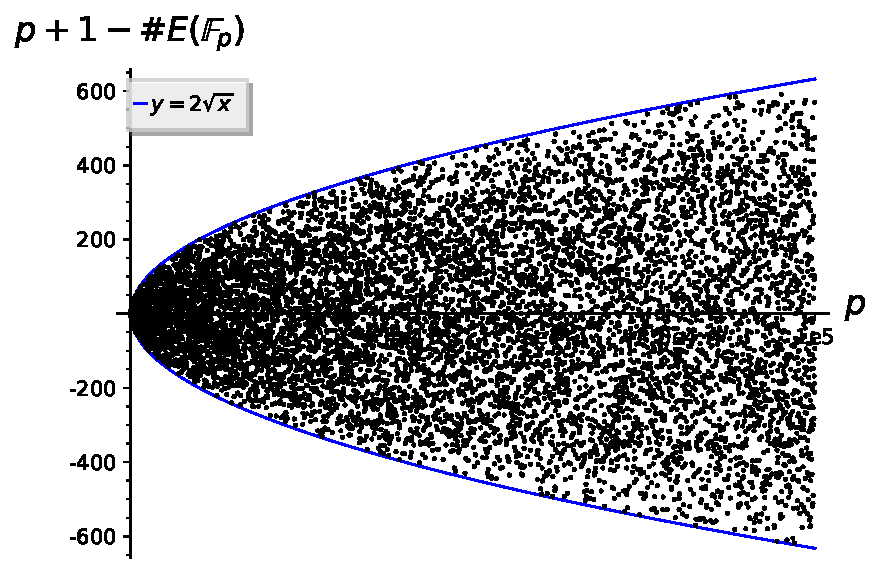
\includegraphics[height=.3\textheight]{pointcounts.pdf}
\caption{Il·lustració del Teorema de Hasse per la corba $E\colon y^2=x^3-x+1$}
\end{figure}
\end{example}

\begin{theorem}[Teorema de Hasse]
 Si $E$ és una corba el·líptica definida sobre $\F_q$, aleshores
 \[
 |\# E(\F_q) - (q+1)|\leq 2\sqrt{q}.
 \]
\end{theorem}

En la demostració del teorema anterior, és crucial estudiar la isogènia següent (les aplicacions entre corbes el·líptiques que són algebraiques i que a més preserven l'estructura de grup s'anomenen \emph{isogènies}):

\begin{definition}
Sigui $E/\F_q$ una corba el·líptica. L'\emph{endomorfisme de Frobenius} és la isogènia
\[
\phi_E\colon E\to E,\quad (x,y)\mapsto(x^q,y^q).
\]
\end{definition}

\begin{remark}
Observem que si $(x,y)\in E(\bar\F_q)$ satisfà l'equació de la corba, posem
\[
y^2=x^3+ax+b,
\]
aleshores
\[
y^2q = (x^3+ax+b)^q = (x^q)^3 + a^q x^q + b^q = (x^q)^3 + ax^q + b,
\]
on hem fet servir que $q$ és una potència de $p$ (i $p$ és la característica del cos), el teorema del ``binomi del Batxillerat'' i el fet que $a$ i $b$ són de $\F_q$.
\end{remark}

\begin{proof}[Idea de la demostració del Teorema de Hasse]
Es basa en tres fets fonamentals, la demostració dels quals ometrem.
\begin{enumerate}
    \item A cada isogènia $\varphi\in \End(E)$ se li pot assignar un grau $\deg(\varphi)$.
    \item $\deg(\phi_E)=q$ i $\deg([m])=m^2$ per a tot $m\in\Z$,
    \item La isogènia $\phi_E-1$ té nucli de tamany $\deg(\phi_E-1)$, i
    \item $\deg\colon\End(E)\to\Z$ és una forma quadràtica.
\end{enumerate}
La desigualtat de Cauchy--Schwartz diu aleshores que donades isogènies $\varphi_1$ i $\varphi_2$ es té
\[
|\deg(\varphi_1-\varphi_2)-\deg(\varphi_1)-\deg(\varphi_2)|\leq 2\sqrt{\deg(\varphi_1)\deg(\varphi_2)}.
\]
Aplicant aquesta desigualtat a $\varphi_1=\phi_E$ i $\varphi_2=[1]$ obtenim el resultat, ja que $\#E(\F_q)=\#\ker(\phi_E-1)=\deg(\phi_E-1)$.
\end{proof}
\begin{proposition}
 Sigui $E/\F_q$ una corba el·líptica, i escrivim $a= q+1 - \#E(\F_q)$. Aleshores $\phi_E$ satisfà
\[
\phi_E^2 - a\phi_E + q =0.
\]
\end{proposition}

\begin{remark}
La proposició diu que per a tot punt $P=(x,y) \in E(\bar\F_q)$, es té
\[
(x^{q^2},y^{q^2}) - a\cdot (x^q,y^q) + q\cdot(x,y) = \calO.
\]
Aquí, recordem que les operacions $-$ i $+$ i $\cdot$ es corresponen a la llei de grup.
\end{remark}

El següent teorema ens dona una manera fàcil de calcular $\#E(\F_{q^n})$ si la corba $E$ està definida sobre $\F_q$ i sabem calcular $\#E(\F_q)$. Considerem el polinomi $X^2-aX + q$, on $a=q+1-\# E(\F_q)$, que té discriminant $a^2-4q \leq 0$ pel Teorema de Hasse. Per tant, les seves arrels $\alpha,\beta\in\C$ són complexes conjugats, i el seu producte és $q$, per tant $|\alpha|=|\beta|=\sqrt{q}$.
\begin{theorem}
 Sigui $E$ una corba el·líptica definida sobre $\F_q$. Aleshores,
 \[
 \# E(\F_{q^n}) = q^n + 1 - \alpha^n - \beta^n,\quad \forall n\geq 1.
 \]
\end{theorem}
 
% També ens podem preguntar per l'estructura de grup d'$E(\F_q)$.
 
% \begin{theorem}
%  El grup $E(\F_q)$ és el producte de dos grups cíclics. Per tant, si escrivim $N=\#E(\F_q)$, tenim
%  \[
%  E(\F_q) \cong \prod_{p\mid N} \Z/p^\alpha_p\Z \times \Z/p^\beta_p\Z,
%  \]
%  on $\alpha_p\geq 1$ i $\beta_p\geq 0$ per a tot $p\mid N$.
% \end{theorem}
 
 \subsection{Criptografia amb corbes el·líptiques}
 
 \subsubsection{Diffie--Hellman amb corbes el·líptiques}
 Recordem que el protocol de Diffie--Hellman fa servir l'operació de grup a $\F_p^\times$, que és un grup cíclic, per establir una clau comuna entre Alice i Bob. Podem canviar el grup $\F_p^\times$ pel grup generat per un punt $P\in E(\F_q)$. Denotem per $N$ l'ordre del punt $P$ (fixem-nos que $N\simeq q$, pel teorema de Hasse). Això resulta en el següent protocol (compareu-lo amb la \S\ref{sec:diffie-hellman}).
 
 \begin{enumerate}
    \item L'Alice escull un enter a l'atzar $1<a<N$, i envia el punt $Q_A=aP\in E(\F_q)$ a en Bob.
    \item En Bob, per la seva banda, escull un enter a l'atzar $1<b<N$, i envia el punt $Q_B=bP\in E(\F_q)$ a l'Alice.
    \item L'Alice i en Bob calculen respectivament $aQ_B$ i $bQ_A$. Observem que els dos punts calculats són iguals a $abP$, que serà el secret compartit.
\end{enumerate}

En aquest cas, també es creu que \emph{problema de Diffie--Hellman per corbes el·líptiques (ECDHP)} i el \emph{problema del logaritme discret per corbes el·líptiques (ECDLP)} són equivalents. Òbviament, la seguretat del sistema depèn de l'ordre $N$ del punt $P$ escollit, i per tant ens interessarà trobar corbes el·líptiques $E/\F_q$ tals que $\#E(\F_q)$ sigui divisible per un primer gran.

Per altra banda, l'algoritme més potent per resoldre el logaritme discret a $\F_q^\times$, que s'anomena ``Index Calculus'', no té anàleg a $E(\F_q)$. Això fa que per solucionar el logaritme discret a $E(\F_q)$ només es tinguin disponibles els algoritmes que funcionen per grups cyclic genèrics. Conseqüentment, un sistema criptogràfic basat en l'ECDLP pugui assolir la mateixa seguretat que un sistema basat en el DLP treballant amb un cos finit de cardinal molt menor.

La companyia Certicom\footnote{\url{https://www.certicom.com/content/certicom/en/the-certicom-ecc-challenge.html}} té diferents reptes de resoldre el logaritme discret en corbes el·líptiques, i ofereix 20.000\$ a qui trobi el logaritme discret d'un punt concret d'una corba $E$ definida sobre $\F_p$, on $p=1550031797834347859248576414813139942411$ (131 bits). En canvi, des del 2005 es pot (amb tècniques molt avançades i amb molt d'esforç computacional) resoldre el logaritme discret per primers d'aquest tamany. De fet, es pot fer per primers de fins a 180 bits. Es considera que la seguretat en corbes el·líptiques obtinguda amb primers d'uns 160 bits és comprable a l'obtinguda a $\F_p^\times$ amb primers de 1024 bits, mentre que amb només 256 bits s'obté la seguretat corresponent a 4096 bits de $\F_p^\times$.

 \subsubsection{ElGamal amb corbes el·líptiques}
 Una variant del protocol de Diffie--Hellman ens permet establir un sistema de xifrat de clau pública basat en el logaritme discret. El descriurem de manera uniforme per  un grup $G=\F_q^\times$ o $G=E(\F_q)$.
 
 \begin{description}
 \item[Preparació: ] Cada usuari (posem Alice) tria un element $g\in G$ d'ordre $N$ suficientment gran. Seguidament, tria un enter $2< a < N$ i calcula $A=g^a$. La clau pública de l'Alice serà la tupla $(G,g,A)$, i la clau secreta serà $a$.
 \item[Xifrat: ] Suposem que en Bob vol enviar un missatge $m\in G$ a l'Alice. En Bob tria un enter a l'atzar, $2< y < N$, i calcula $Y=g^y\in G$ i també $Z=mA^y$. Aleshores envia a Alice la tupla $(Y,Z)$.
 \item[Desxifrat: ] Per recuperar el missatge, Alice calcula $Y^{-a} Z$. Observem que
 \[
 Y^{-a}Z = g^{-ay}mg^{ay} = m.
 \]
 \end{description}
 Fixem-nos que la part de preparació s'assembla molt al que fa l'Alice amb el protocol Diffie--Hellman, mentre que la part de xifrat s'assembla al que faria en Bob, amb la diferència que la part ``secreta`` $y$ va canviant a cada missatge. Aleshores la part ``pública'' $Y$ permet acordar un secret comú (que seria $Y^a=g^{ay}=A^y$), i que és justament el secret que s'ha fet servir per emmascarar el missatge $m$.
 
 Si un possible atacant que tingui accés a la comunicació vol recuperar el missatge $m$ a partir de $(Y,Z)$, haurà de trobar el secret a partir de $Y=g^y$ i de $A=g^a$, i això és precisament el problema de Diffie--Hellman, que estem assumint igual de difícil que el problema del logaritme discret.
 
 \subsection{Comptatge de punts}
 En aquest apartat volem estudiar el problema de determinar, donada una corba $E/\F_p$, el nombre de punts $\# E(\F_p)$. Ja sabem que, pel Teorema de Hasse,
 \[
 \# E(\F_p) = p + 1 - t,\quad |t|\leq 2\sqrt{p}.
 \]
 Suposem també que $p>3$ (en cas contrari, és molt fàcil determinar $E(\F_p)$), i escrivim $E$ en la forma
 \[
 E\colon y^2=x^3+Ax+B, \quad A,B\in\F_p.
 \]
 Per cada $a\in \F_p$, definim
 \[
 \chi(a)=\begin{cases}
 0&\text{si } a=0,\\
 +1&\text{si } a\in(\F_p^\times)^2,\\
 -1&\text{si } a\in \F_p^\times\smallsetminus (\F_p^\times)^2.
 \end{cases}
 \]
 Aleshores, observem que
 \[
 \# E(\F_p) = 1+ \sum_{x\in\F_p} (1+\chi(x^3+Ax+B))= 1+p+\sum_{x\in\F_p} \chi(x^3+Ax+B),
 \]
 i per tant tenim una formula tancada per $t$:
 \[
 t = \sum_{x\in\F_p}\chi(x^3+Ax+B).
 \]
 A la secció següent veurem una manera eficient de calcular $\chi(x)$ per qualsevol $x\in\F_p$. Tot i així, si $p$ és molt gran (de manera que ens sigui útil en criptografia) no podrem recórrer\footnote{En l'actualitat es fan servir primeres d'entre $50$ i $80$ xifres decimals, i cal tenir en compte que un ordinador actual trigaria l'edat de l'univers a recórrer els enters entre $1$ i $10^{27}$.} tots els elements de $\F_p$.
 
 \subsubsection{L'algoritme d'Schoof}
 El 1985, R.~Schoof va donar el primer algoritme que calculava $\#E(\F_p)$ amb un nombre d'operacions polinomial en $\log(p)$, fet que va permetre d'utilitzar les corbes el·líptiques en la criptografia de manera pràctica. Seguidament veurem les idees principals de l'algoritme d'Schoof.
 
 Recordem que l'endomorfisme de Frobenius
 \[
 \phi\colon E\to E,\quad (x,y)\mapsto (x^p,y^p)
 \]
 satisfà l'equació quadràtica
 \[
 \phi^2-t\phi+q = 0.
 \]
 Sigui $P=(x,y)\in E(K)$, on $K/\F_p$ és una extensió qualsevol. Aleshores
 \begin{align}
 \label{eq:frobenius-schoof}
 (x^{p^2},y^{p^2}) + [p] (x,y) = [t] (x^p,y^p).
 \end{align}
 La quantitat de l'esquerra es pot calcular de manera eficient, fent servir exponenciació modular pel primer terme, i l'anàleg de l'exponenciació modular per corbes el·líptiques pel segon.
 
 \begin{remark}
 Fixem-nos que l'enter $t$ no es pot extreure directament de $[t]$, ja que si $(x,y)$ té ordre $N$, aleshores $(x^p,y^p)$ també (per què?), i per tant $[t+kN](x^p,y^p)=[t](x^p,y^p)$ per a tot $k$. Així, només podem determinar $t$ mòdul $N$. 
 \end{remark}
 
 La idea de Schoof consisteix en determinar $t\pmod \ell$ per suficients primers $\ell$ petits, i després reconstruir $t$ fent servir el teorema xinès dels residus. Per exemple, per determinar $\#E(\F_p)$ amb $p\simeq 10^{71}$ n'hi ha prou amb considerar $2<\ell<100$. Afegint-hi els 5 primers que hi ha fins a $\ell < 115$ ja podem determinar $\#E(\F_p)$ amb $p\simeq 10^{91}$, i amb dos primers més ($127$, $131$) ja podem arribar a $p\simeq 10^{100}$.
 
 Fem primer el cas $\ell=2$.
 \begin{lemma}
  \[
  t\bmod 2=\begin{cases}
  1 & \text{si } x^3+Ax+B\text{ és irreductible a } \F_p,\\
  0 & \text{altrament.}
  \end{cases}
  \]
 \end{lemma}
\begin{proof}
 Recordem que $x^3+Ax+B$ factoritza a $\F_p$ si i només si $E(\F_p)$ té un element d'ordre $2$ (que és $(\alpha,0)$ on $\alpha$ és una arrel de $x^3+Ax+B$). Ara bé, com que $p$ és senar tenim
 \[
 \# E(\F_p) = p+1-t\equiv t\pmod 2,
 \]
 i $E(\F_p)$ té un element d'ordre $2$ si i només si $\#E(\F_p)$ és parell.
 \end{proof}
 
 Així, considerem ara un primer $\ell$ senar, i ens cal trobar un punt d'ordre $\ell$. No podem esperar que aquest punt estigui definit a $\F_p$, i per tant en general haurem de considerar extensions $K/\F_p$. 
 
 \begin{theorem}
  Considerem els polinomis $\psi_m\in\F_p[x,y]$,
  \begin{align*}
  \psi_1&=1,\quad \psi_2=2y,\\
  \psi_3 &= 3x^4+6Ax^2+12Bx-A^2,\\
  \psi_4&=4y(x^6+5Ax^4+20Bx^3-5A^2x^2-4ABx-8B^2-A^3),\\
  \psi_{2m+1}&=\psi_{m+2}\psi_{m}^3 - \psi_{m-1}\psi_{m+1}^3,& (m\geq 2),\\
  \psi_{2m}&=\frac{\psi_m}{2y}(\psi_{m+2}\psi_{m-1}^2-\psi_{m-2}\psi_{m+1}^2),& (m\geq 3).
  \end{align*}
  Aleshores per a tot primer senar $\ell<p$, $\psi_\ell\in \F_p[x,y^2]$ i, si substituim $y^2=x^3+Ax+B$ obtenim un polinomi en $x$ de grau $\frac{\ell^2-1}{2}$. A més,
  \[
  P\in E(\bar\F_p)[\ell]\smallsetminus\{\calO\}\iff \psi_\ell(x(P))=0. 
  \]
 \end{theorem}
 \begin{corollary}
 Per tot primer $\ell$, es té
  \[
  E[\ell]\cong\Z/\ell\Z\oplus\Z/\ell\Z.
  \]
 \end{corollary}
 \begin{proof}
  Els punts d'$E[\ell]=E(\bar\F_p)[\ell]$ són de la forma $(\alpha, \beta)$ on $\alpha$ és una arrel de $\psi_\ell$. Per tant, hi ha $1+2\deg(\psi_\ell)=\ell^2$ punts a $E[\ell]$. Com que tot $P\in E[\ell]$ satisfà $\ell P=\calO$, necessàriament $E[\ell]=\Z/\ell\Z\oplus\Z/\ell\Z$.
 \end{proof}
 Si prenem $K/\F_p$ un cos on $\psi_\ell$ tingui alguna arrel $\alpha$, aleshores podem considerar el punt de $\ell$-torsió $P=(\alpha,\sqrt{D})\in E(K(\sqrt{D}))$, on $D=\alpha^3+A\alpha+B$.
 
 La següent millora ens permet treballar al cos $K$, sense afegir una arrel de $D$. Considerem la corba
 \[
 E^D \colon y^2 = x^3 + AD^2x + BD^3.
 \]
 Aleshores l'isomorfisme
 \[
 \tau\colon E\to E^D,\quad (x,y\delta)\mapsto (Dx,D^2y), \quad \delta=\sqrt{D}
 \]
 ens permet realitzar totes les operacions a $E^D(K)$. Observem que
\begin{align*}
    \tau((\alpha,\delta)) &= (D\alpha, D^2),\\
    \tau((\alpha^p,\delta^p)) &=(D\alpha^p,D^{\frac{p+3}{2}}),\\
    \tau((\alpha^{p^2},\delta^{p^2})) &=(D\alpha^{p^2},D^{\frac{p^2+3}{2}}).
\end{align*}
Per tant, l'equació~\eqref{eq:frobenius-schoof} és equivalent a la següent equació a $E^D$:
\[
(D\alpha^{p^2},D^{\frac{p^2+3}{2}}) + [p] (D\alpha,D^2) = [t] (D\alpha^p,D^{\frac{p+3}{2}}).
\]

Vegem la complexitat d'aquest algoritme. Els polinomis $\psi_\ell$ tenen grau $O(\ell^2)=O(\log^2 p)$. Per tant, els elements de l'extensió $K$ tenen tamany $O(\ell^2\log q)=O(\log^3 q)$. Per calcular $\alpha^p$ i $\alpha^{p^2}$ calen $O(\log p)$ operacions a $K$, i per tant en total $O((\log p)(\log^3 p)^2)$, és a dir $O(\log^7 p)$. Com que això s'ha de fer per $O(\log p)$ primers (pel Teorema dels Nombres Primers), en total calen $O(\log^8 p)$ operacions de bit. Si es poden fer operacions a $K$ de manera més ràpida (per exemple fent servir transformades de Fourier) es pot reduir la complexitat a $O(\log^{5+\epsilon} p)$. Millores posteriors de Elkies i Atkin permeten calcular $\#E(\F_p)$ amb temps $O(\log^{4+\epsilon} p)$.

Acabem la secció amb una implementació en  \texttt{Sage} de l'algoritme d'Schoof.

\begin{python}    
def t_mod(A, B, p, ell):
    pmod = p % ell
    if pmod > ell / 2: pmod -= ell
    R.<t> = PolynomialRing(GF(p)))
    if ell == 2: return 1 if (t^3+A*t+B).is_irreducible() else 0
    h = E.division_polynomial(ell,t,0).factor()[0][0]
    K.<a> = FiniteField(p^h.degree(), modulus = h)    # K = F[x]/(h(x))
    D = a^3 + A * a + B
    E = EllipticCurve([A*D^2, B*D^3])
    P = E([D*a,D^2])
    phi_P = E([D * a^p, D^((p+3)//2)])
    phi2_P = E([D * a^(p^2), D^((p^2+3)//2)])
    LHS = phi2_P + pmod * P; RHS = E(0)
    for t in xrange((ell+1)//2):
        if LHS ==  RHS: return t
        elif LHS == -RHS: return -t
        RHS += phi_P
\end{python}
\begin{python}
def Schoof(A, B, p): # y^2 = x^3 + Ax + B 
    M = 1; ell = 1; S = []; traces = []
    while M <= 4*RR(p).sqrt():
        ell = next_prime(ell); S.append(ell); M *= ell
        traces.append(t_mod(A, B, p, ell))      
    t = CRT(traces, S) # Fem servir el Teorema Xinès dels Residus
    return t if t < M / 2 else t-M
\end{python}
}
%\chapterimage{Cap2.png}
\chapter{La llei de reciprocitat quadràtica (\texorpdfstring{$\sim$5h}{})}
{
\let\paragraph\subsubsection
\let\subsubsection\subsection
\let\subsection\section

\subsection{Residus quadràtics i el símbol de Legendre}

L'objectiu d'aquesta secció és estudiar les solucions d'equacions quadràtiques mòdul un primer $p$. Concretament, ens fixarem en l'equació $x^2\equiv a\pmod{p}$.

\begin{definition}
 Sigui $p$ un primer. Diem que un enter $a$ no divisible per $p$ és un \emph{residu quadràtic mòdul $p$} si $a$ és un quadrat mòdul $p$. Si no, direm que $a$ és un \emph{no-residu quadràtic mòdul $p$}.
\end{definition}

Òbviament, si $a\equiv a'\pmod{p}$ aleshores $a$ és un residu quadràtic mòdul $p$ si i només si $a'$ ho és.

\begin{example}
L'$1$ és l'únic residu quadràtic tant mòdul $2$ com mòdul $3$.
Els residus quadràtics mòdul $5$ són l'$1$ i el $4$, perquè $1^2\equiv 1$, $2^2\equiv 4$, i $3^2\equiv (-2)^2$, $4^2 \equiv (-1)^2$.

Els residus quadràtics mòdul $7$ són $\{1,2,4\}$.

Els residus quadràtics mòdul $11$ són $\{1,3,4,5,9\}$.
\end{example}

Introduim una notació que va bé per parlar d'aquest concepte.

\begin{definition}
El \emph{símbol de Legendre} es defineix, donats un primer \textbf{senar} $p$ i un enter $a$, com
\[
\legendre{a}{p}=\begin{cases}
0 &\text{ si } p\mid a,\\
+1 &\text{ si $a$ és un residu quadràtic mòdul $p$,}\\
-1&\text{ si $a$ és un no-residu quadràtic mòdul $p$}.
\end{cases}
\]
\end{definition}

Si $a$ i $b$ són residus quadràtics, posem $a\equiv x^2\pmod p$ i $b\equiv y^2\pmod p$, aleshores és clar que $ab\equiv (xy)^2\pmod p$ i, per tant $ab$ també és un residu quadràtic. De manera semblant, si $a\equiv x^2\pmod p$ i $ab\equiv y^2\pmod p$, aleshores $b\equiv (x^{-1}y)^2\pmod p$, del que en deduïm que el produce d'un residu amb un no-residu és un no-residu. El següent lema ens diu que el producte de dos no-residus és un residu.
\begin{lemma}
Si $p$ és un primer senar, l'aplicació $\psi\colon (\Z/p\Z)^\times \to \{\pm 1\},\quad a\mapsto \legendre{a}{p}$ és un morfisme de grups exhaustiu.
\end{lemma}
\begin{proof}
Fem servir que $G = (\Z/p\Z)^\times$ és cíclic. El nucli de l'aplicació $\psi$ el formen els quadrats, un subgrup (normal) $H$ d'índex $2$. Per tant $\psi$ és la composició de
\[
G\surjects G/H \cong \{\pm 1\}.
\]
\end{proof}

\subsection{LRQ i demostració}

Durant el segle XVIII, els matemàtics es van preguntar si hi havia una manera senzilla de predir com es comporta $\legendre{a}{p}$ quan variava $p$. Per exemple, quan $a=5$ podem fer una taula com la que apareix a la Taula~\ref{taula:lrq}.
\begin{table}[ht]
\centering
\label{taula:lrq}
\begin{tabular}{lcccccccccccc}
\toprule
    $p$ & 7  & \textbf{11} & 13 & 17 & \textbf{19} & 23 & \textbf{29} & \textbf{31} & 37 & \textbf{41} & 43 & 47\\
    \midrule
    $\legendre{5}{p}$& -1& \textbf{1}& -1 & -1 & \textbf{1} & -1 & \textbf{1} & \textbf{1} & -1 & \textbf{1} & -1 & -1\\
    $p\bmod 5$ & 2 & \textbf{1} & 3 & 2 & \textbf{4} & 3 &\textbf{4} & \textbf{1} & 2 &\textbf{1} & 3 & 2\\
    \bottomrule
\end{tabular}
\caption{Taula de $\legendre{5}{p}$ per diversos primers.}
\end{table}
Fixem-nos que sembla que el símbol $\legendre{5}{p}$ només depengui de si $p\equiv 1,4\pmod{5}$ o no. En canvi, si fem el mateix amb $a=7$ obtenim la Taula~\ref{taula:lrq2}.
\begin{table}[ht]
\label{taula:lrq2}
\centering

\begin{tabular}{lcccccccccccccc}
\toprule
    $p$ & 11 & 13 & 17 & \textbf{19} & 23 & \textbf{29} & \textbf{31} & \textbf{37} & 41 & 43 & \textbf{47}&\textbf{53}&\textbf{59}&61\\
\midrule
    $\legendre{7}{p}$& -1& -1& -1 & \textbf{1} & -1 & \textbf{1} & \textbf{1} & \textbf{1} & -1 & -1 & \textbf{1} & \textbf{1} & \textbf{1}&-1\\
    $p\bmod 7$ & 4 & 6 & 3 & \textbf{5} & 2& \textbf{1} & \textbf{3} & \textbf{2} & 6 & 1 & \textbf{5} & \textbf{4} & \textbf{3}&5\\
\bottomrule
\end{tabular}

\caption{Taula de $\legendre{7}{p}$ per diversos primers.}

\end{table}
Ara observem que no sembla d'entrada que hi hagi una relació tan senzilla. En canvi, per $a=11$ tornem a observar el mateix comportament que per $a=5$ (quant val $\legendre{9}{p}$?). El teorema següent explica aquest fenòmen de manera molt precisa.

\begin{theorem}[Llei de Reciprocitat Quadràtica de Gauss]
\label{thm:lrq}
Siguin $p$ i $q$ dos primers senars. Aleshores
\[
    \legendre{p}{q} = (-1)^{\frac{p-1}{2}\frac{q-1}{2}}\legendre{q}{p}=\begin{cases}
    +\legendre{q}{p} & p\equiv 1\pmod 4\text{ o } q\equiv 1 \pmod{4}\\
    -\legendre{q}{p} & p\equiv 3\pmod 4\text{ i } q\equiv 3 \pmod{4}
    \end{cases}.
    \]
A més,
\[
\legendre{-1}{p} = (-1)^{\frac{p-1}{2}}=\begin{cases}
+1&p\equiv 1\pmod{4}\\
-1&p\equiv 3\pmod{4},
\end{cases}
\quad
\legendre{2}{p} = \begin{cases}
+1 & p\equiv \pm 1\pmod {8}\\
-1 & p \equiv \pm 3 \pmod{8}.
\end{cases}
\]
\end{theorem}

Fixem-nos que, si posem $p=5$, el teorema anterior ens dona que
\[
\legendre{5}{p} = \legendre{p}{5} = \begin{cases}
+1 &p\equiv 1,4\pmod 5,\\
-1 &p\equiv 2,3\pmod 5.
\end{cases}
\]
En canvi, si $p=7$, el signe $(-1)^{\frac{p-1}{2}\frac{q-1}{2}}= (-1)^{\frac{q+1}{2}}$ depèn de com sigui $q$ mòdul $4$. Com que $\legendre{q}{7}$ depèn de $q$ mòdul $7$, la quantitat $\legendre{7}{q}$ depèn de $q$ mòdul $28$. De fet,
\[
\legendre{7}{p}=\begin{cases}
1&p\equiv 1, 3, 9, 19, 25, 27\pmod{28}\\
-1&p\equiv 5, 11, 13, 15, 17, 23\pmod{28}\\
0 & p = 7.
\end{cases}
\]

La LRQ també ens permet calcular ràpidament els símbols de Legendre: per exemple, suposem que volem saber si $211$ és un quadrat mòdul $653$.

Com que $653\equiv 1\pmod 4$,
\[
\legendre{211}{653}=\legendre{653}{211},
\]
i com que $653\equiv 20\pmod{211}$,
\[
\legendre{653}{211} = \legendre{20}{211}=\legendre{4\cdot 5}{211} = \legendre{4}{211}\legendre{5}{211}=\legendre{5}{211}.
\]
Com que $5\equiv 1\pmod 4$,
\[
\legendre{5}{211}=\legendre{211}{5}=\legendre{1}{5} = 1.
\]
Concloem que $211$ és un quadrat mòdul $653$, però fixem-nos que aquest càlcul no ens permet dir quin és $x$ tal que $x^2\equiv 211\pmod{653}$ (solució: $118^2\equiv 211\pmod{653}$).

Fixem-nos que per dur a terme el càlcul anterior cal factoritzar ($20=4\cdot 5$). Per nombres molt grans això seria un problema, però hi ha una generalització del símbol de Legendre (anomenat símbol de Jacobi) que solventa aquest problema.

\subsubsection{Demostració de la LRQ}

Sigui $p$ un primer senar, i $a$ un enter no divisible per $p$. El primer resultat que ens caldrà dona una manera eficient de calcular $\legendre{a}{p}$, i ens servirà també per la demostració de la LRQ.
\begin{proposition}[Criteri d'Euler]
 \[
 \legendre a p \equiv a^{\frac{p-1}{2}}\pmod p.
 \]
\end{proposition}
\begin{proof}
Si $a\equiv x^2\pmod p$, aleshores
\[
a^{\frac{p-1}{2}} \equiv x^{p-1}\equiv 1\pmod p,
\]
pel petit teorema de Fermat. Considerem ara la factorització
\[
x^{p-1}-1 = (x^{\frac{p-1}{2}}-1)(x^{\frac{p-1}{2}}+1).
\]
El polinomi $x^{p-1}-1$ té com a molt $p-1$ arrels a $\Z/p\Z$. Com que tots els elements de $(\Z/p\Z)^\times$ en són arrel, en deduïm que té exactament $p-1$ arrels. Aquestes s'han de dividir en arrels de cadascun dels factors. Com que la meitat d'elements (els quadrats) són arrel del primer factor, l'altra meitat (els no-quadrats) han de ser arrels del segon factor, i per tant si $a$ és un no-quadrat,
\[
a^{\frac{p-1}{2}}+1\equiv0\pmod p,
\]
com voliem veure.
\end{proof}

Observem que la proposició anterior demostra la fórmula per $\legendre{-1}{p}$. Vegem ara la fórmula per $\legendre{2}{p}$.

\begin{proposition}
Si $p$ és un primer senar, aleshores
\[
\legendre 2p=\epsilon(p)=\begin{cases}
+1&p\equiv \pm 1\pmod{8},\\
-1&p\equiv \pm 3 \pmod{8}.
\end{cases}
\]
\end{proposition}
\begin{proof}
Considerem l'anell $R=\Z[\zeta]/(p)$ amb $\zeta=\zeta_8$. Pel criteri d'Euler,
\[
\legendre{2}{p}\equiv 2^{\frac{p-1}{2}}\pmod p,
\]
i per tant serà útil trobar una arrel quadrada de $2$ mòdul $p$. Fixem-nos que $\zeta^4+1=0$, o $\zeta^2+\zeta^{-2}=0$. Per tant, si escrivim $\tau=\zeta+\zeta^{-1}$, tenim
\[
\tau^2 = (\zeta+\zeta^{-1})^2= 2.
\]
Deduïm que
\[
2^{\frac{p-1}{2}}\equiv \tau^{p-1}\pmod p.
\]
Veurem ara que $\tau^p\equiv \zeta^p+\zeta^{-p}\equiv \epsilon(p)\tau\pmod p$:
\begin{description}
\item[Cas $p\equiv \pm 1\pmod 8$ ($\iff \epsilon(p)=1$):] En aquest cas, $\tau^p\equiv \zeta+\zeta^{-1}\equiv \tau\pmod p$.
\item[Cas $p\equiv \pm 3\pmod 8$ ($\iff \epsilon(p)=-1$):] En aquest cas, $\tau^p\equiv \zeta^3+\zeta^{-3}\equiv -\tau\pmod p$.
\end{description}
Per tant, $\tau \legendre{2}{p} \equiv \epsilon(p) \tau \pmod p$ i, multiplicant per $\tau$, obtenim
\[
2\legendre{2}{p}\equiv 2\epsilon(p)\pmod p.
\]
Com que $p$ és senar, trobem finalment $\legendre{2}{p}=\epsilon(p)$.
\end{proof}


Donat un primer $p$, denotarem per $\zeta_p$ el nombre complex $\zeta_p=e^{\frac{2\pi i}{p}}$. Recordem una propietat coneguda de $\zeta_p$:

\begin{lemma}
Es té, per a tot $a\in \Z$,
\[
\sum_{n=0}^{p-1} \zeta_p^{an}=\begin{cases}
p& p\mid a,\\
0& p\nmid a.
\end{cases}
\]
\end{lemma}
\begin{proof}
Si $p\mid a$, aleshores $\zeta_p^a=1$ i el resultat és obvi. En cas contrari, $\zeta_p^a\neq 1$, i per tant la suma geomètrica val
\[
\sum_{n=0}^{p-1} \zeta_p^{an} = \frac{\zeta_p^{ap}-1}{\zeta_p^a-1}=0.
\]
\end{proof}

\begin{definition}
 La \emph{suma de Gauss} associada a un element $a\in (\Z/p\Z)^\times$ és
 \[
 \gamma_a = \sum_{n=1}^{p-1}\legendre{n}{p} \zeta_p^{an}.
 \]
\end{definition}

\begin{lemma}
La suma de Gauss $\gamma_0$ val $0$.
\end{lemma}
\begin{proof}
Com que $\gamma_0=\sum_{n=1}^{p-1} \legendre{n}{p}$ i hi ha la meitat d'elements que són residus quadràtics i la meitat que no ho són, la suma dels residus és $0$.
\end{proof}

\begin{lemma}
Per a tot enter $a$, es té $\gamma_a=\legendre{a}{p}\gamma_1$.
\end{lemma}
\begin{proof}
Pel lema anterior, podem assumir que $p\nmid a$. Aleshores:
\[
\legendre a p\sum_{n=0}^{p-1} \legendre n p \zeta_{p}^{an}= \sum_{n=0}^{p-1} \legendre{an}{p}\zeta_p^{an} = \sum_{m=0}^{p-1} \legendre{m}{p}\zeta_p^m = \gamma_1,
\]
on hem fet servir que multiplicar per $a$ permuta els elements de $\Z/p\Z$. El resultat s'obté multiplicant per $\legendre ap$.
\end{proof}

La base de la demostració és el següent resultat.
\begin{proposition}
Per tot enter $a$ coprimer amb $p$, es té que
 \[
 \gamma_a^2 = (-1)^{\frac{p-1}{2}} p.
 \]
\end{proposition}
\begin{proof}
 Pel lema anterior, podem suposar que $a=1$. Fixem-nos que, pel criteri d'Euler,
 \[
 \gamma_a\gamma_{-a}=\legendre{a}{p}\gamma_1\legendre{-a}{p}\gamma_1=\legendre{-1}{p}\gamma_1^2 = (-1)^{\frac{p-1}{2}} \gamma_1^2.
 \]
 Per tant, caldrà veure que $\gamma_a\gamma_{-a} = p$. Per fer-ho, calculem (totes les sumes recorren els enters entre $1$ i $p-1$).
 \begin{align*}
     \sum_a \gamma_a\gamma_{-a} &= \sum_{a,m,n} \legendre{n}{p}\legendre{m}{p}\zeta_p^{an-am}\\
     &=\sum_{n,m} \legendre{n}{p} \legendre{m}{p} \sum_{a} \zeta^{a(n-m)} = \sum_n p \legendre{n}{p}^2 = p(p-1).
 \end{align*}
\end{proof}

\begin{proof}[Demostració del Teorema~\ref{thm:lrq}]
Si escrivim $p^*=(-1)^{\frac{p-1}{2}} p$, aleshores fixem-nos que
\[
\legendre{p^*}{q} = \legendre{-1}{q}^{\frac{p-1}{2}} \legendre pq \equiv (-1)^{\frac{p-1}{2}\frac{q-1}{2}} \legendre pq \pmod q.
\]
Per tant, per demostrar la LRQ ens cal veure que
\[
\legendre{p^*}{q} \equiv \legendre{q}{p} \pmod{q}.
\]
Per acabar, haurem de treballar a $\Z[\zeta_p]/(q)$, que és un anell de característica $q$. Aleshores, pel criteri d'Euler,
\[
\gamma_1\legendre{p^*}{q}\equiv \gamma_1(p^*)^{\frac{q-1}{2}} \equiv \gamma_1^q\pmod{q}.
\]
Ara calculem
\begin{align*}
\gamma_1^q &\equiv \left(\sum_n \legendre{n}{p}\zeta_p^n\right)^q \equiv \sum_n \legendre{n}{q} \zeta_p^{qn} \equiv \gamma_q\equiv \gamma_1\legendre{q}{p}\pmod{q}.
\end{align*}
Com que $\gamma_1$ és invertible a $\Z[\zeta_p]/(q)$, podem simplificar $\gamma_1$ de l'expressió
\[
\gamma_1\legendre{p^*}{q}\equiv \gamma_1 \legendre{q}{p}\pmod{q}
\]
per obtenir el resultat.

\end{proof}

\subsection{El símbol de Jacobi}
Donats un enter $a$ i un \emph{enter senar positiu} $m$, definim
\[
\legendre{a}{m}=\prod_{p^k\parallel m} \legendre{a}{p}^k,
\]
on en el producte de la dreta el símbol és el de Legendre. Observem que si $m$ és un primer senar, aleshores aquesta definició coincideix amb el símbol de Legendre.

\begin{lemma}
\begin{enumerate}
    \item Si $a\equiv b\pmod m$ aleshores $\legendre{a}{m} = \legendre{b}{m}$.
    \item $\legendre{ab}{m}= \legendre am \legendre bm$ per a qualssevol $a$, $b$ i qualsevol enter senar positiu $m$.
    \item $\legendre{a}{mn} = \legendre am \legendre an$ per a qualsevol $a$ i qualssevol enters senars positius $m$ i $n$.
\end{enumerate}
\end{lemma}
\begin{remark}
 Notem que si $\legendre{a}{m}=-1$ aleshores $a$ no és un quadrat mòdul $m$ (ja que no ho és mòdul $p$ per algun primer $p$ que divideix $m$ a una potència senar). Però en canvi, si $\legendre{a}{m}=1$ no podem deduir que $a$ sigui un quadrat mòdul $m$. Per exemple,
 \[
 \legendre{2}{15} = 1,
 \]
 però els quadrats mòdul $15$ són
 \[
 \{1,4,6,9,10\}.
 \]
\end{remark}


 \begin{theorem}[Llei de Reciprocitat Quadràtica pel símbol de Jacobi]
\label{thm:lrq-jacobi}
Siguin $m$ i $n$ dos enters positius senars i coprimers entre si. Aleshores
\[
    \legendre{m}{n} = (-1)^{\frac{m-1}{2}\frac{n-1}{2}}\legendre{n}{m}.
    \]
A més,
\[
\legendre{-1}{m} = (-1)^{\frac{m-1}{2}}=\begin{cases}
+1&m\equiv 1\pmod{4}\\
-1&m\equiv 3\pmod{4}
\end{cases}
,\quad \legendre{2}{m} = \begin{cases}
1 & m\equiv \pm 1\pmod {8}\\
-1 & m \equiv \pm 3 \pmod{8}.
\end{cases}
\]
\end{theorem}

\begin{example}
 Suposem que volem saber si $7411$ és un quadrat mòdul $9283$. Primer hauriem de veure que els dos són primers (sí que ho són). Aleshores, com que els dos són $\equiv 3\pmod 4$ obtenim
 \[
 \legendre{7411}{9283} = -\legendre{9283}{7411}=-\legendre{1872}{7411}.
 \]
 Si només fem servir el símbol de Legendre, ara hem de factoritzar $1872=2^4\cdot 3^3\cdot 13$. En canvi, fent servir el símbol de Jacobi només hem de treure les potències de $2$:
 \begin{align*}
 &-\legendre{1872}{7411} =-\legendre{2^4}{7411}\legendre{117}{7411} = -\legendre{7411}{117}\\
 &=-\legendre{40}{117} = -\legendre{2}{117}\legendre{5}{117} = \legendre{5}{117}=\legendre{117}{5} = \legendre{2}{5}=-1.
 \end{align*}
\end{example}
 \subsection{Aplicació: arrels quadrades mòdul \texorpdfstring{$p$}{p}}
 \label{sec:arrels-quadrades}
 
 En aquesta secció ens plantegem el problema de trobar les solucions d'una equació quadràtica $ax^2+bx+c=0$ a $\F_p=\Z/p\Z$, amb $p\geq 3$ primer. De la fórmula quadràtica se'n despren que n'hi ha prou amb saber trobar l'arrel quadrada de $D=b^2-4ac$, si en té. Fent servir la llei de reciprocitat quadràtica, hem vist que podem determinar ràpidament si $D$ és un quadrat, però que no obtenim informació sobre com trobar $\delta\in \F$ tal que $\delta^2=D$.
 
 Recordem que, si $D$ és un quadrat, aleshores
 \[
 D^{\frac{p-1}{2}}\equiv 1\pmod p.
 \]
 Per tant, $D^{\frac{p+1}{2}} \equiv D\pmod p$. Observem aleshores que, si $\frac{p+1}{2}$ és parell ($\iff$ $p\equiv 3\pmod 4$), aleshores $\delta=D^{\frac{p+1}{4}}$ satisfà $\delta^2=D$.
 
 Per tant, podem suposar que $p\equiv 1\pmod{4}$. Donarem ara un algoritme probabilístic per trobar $\delta$. Considerem l'anell $R=\F_p[x]/(x^2-D)$, i escrivim $\sqrt{D}$ per la classe de $x$ a $R$. Considerem el morfisme d'anells
 \[
 \varphi\colon R\to \F,\quad a+b\sqrt{D}\mapsto a+b\delta
 \]
 (fixem-nos que encara no hem trobat $\delta$, però en tot cas sabem que existeix).
 
 Ara, triem un element $z\in \F_p^\times$ a l'atzar, i calculem (fent servir exponenciació eficient) la quantitat
 \[
 (1+z\sqrt{D})^{\frac{p-1}{2}}=u+v\sqrt{D}\in R.
 \]
 Com que $\varphi(u+v\sqrt{D}) = (1+\varphi(z)\delta)^{\frac{p-1}{2}}$ i $\F_p^\times$ té $p-1$ elements, necessàriament $u+v\delta\in \{0,1,-1\}$. Per tant, si $v\neq 0$ aleshores
 \[
 \delta\in \{-u/v, (1-u)/v, (-1-u)/v\}.
 \]
 Podem provar aquestes tres possibilitats i trobarem $\delta$. Si $v=0$, triem un altre $z\in \F_p^\times$ i repetim el procés.
 
 \begin{python}
 def troba_arrel_quadrada(a, p):
    assert legendre_symbol(a, p) == 1
    if (p+1) % 4 != 0:
        return a^((p+1)//4)
    S.<x> = GF(p)['x']
    R.<alpha> = S.quotient(x^2-a)
    v = 0
    while v == 0:
        z = GF(p).random_element()
        w = (1 + z*alpha)^ZZ((p-1) / 2)
        u, v = w.list()
    ans = -u / v
    if ans^2 == a:
        return ans
    vinv = 1 / v
    ans += vinv
    if ans^2 == a:
        return ans
    return ans - 2 * vinv
 \end{python}

}
%\chapterimage{Cap3.png}
\chapter{Primalitat i factorització (\texorpdfstring{$\sim$10h}{})}
{
\let\paragraph\subsubsection
\let\subsubsection\subsection
\let\subsection\section


\subsection{Primalitat}

En aquesta secció estudiarem diferents algoritmes que ens permeten decidir si un enter $n$ és primer. És el que es coneix com \emph{tests de primalitat}.

 \subsubsection{El test de Fermat}
 El primer test pràctic que analitzem es basa en explotar el petit Teorema de Fermat. Sabem que si $n$ és primer aleshores per tot enter $a$ amb $\gcd(a,n)=1$ es té $a^{n-1}\equiv 1\pmod n$. Donarem un nom als nombres compostos que es comporten com a primers des del punt de vista d'aquest resultat.
 \begin{definition}
 Un enter compost senar $n$ s'anomena \emph{pseudoprimer en base $a$} si $\gcd(a,n)=1$ i $a^{n-1}\equiv 1\pmod n$.
 \end{definition}
 
 Observem que $n$ és pseudoprimer en bases $a$ i $b$, aleshores també ho és en les bases $ab$ i $ab^{-1}$ (on l'invers el fem mòdul $n$).
 
 \begin{lemma}
 Si $n$ no és pseudoprimer en una base $(a\in\Z/n\Z)^\times$, aleshores $n$ no ho és en com a mínim la meitat de les possibles bases $a$.
 \end{lemma}
 \begin{proof}
  Sigui $\{a_1,\ldots,a_s\}$ el conjunt de les bases en les quals $n$ és pseudoprimer. Sigui $a\in(\Z/n\Z)^\times$ una base en la qual $n$ no és pseudoprimer. Aleshores $\{aa_1,\ldots,aa_s\}$ és un conjunt de $s$ residus tals que $n$ no és pseudoprimer en aquelles bases.
 \end{proof}
 
 \begin{definition}
 Un enter compost $n$ és \emph{de Carmichael} si $n$ és pseudoprimer en totes les bases $b\in(\Z/n\Z)^\times$.
 \end{definition}
 
 Els primers nombres de Carmichael són $561=3\cdot 11\cdot 17$, $1105=5\cdot 13\cdot 17$, $1729 = 7\cdot 13\cdot 19$,\ldots
 
 Per tant, donat un enter senar $n$, si triem $k$ bases $b$ i trobem que
 \[
 b^{n-1}\equiv 1\pmod n
 \]
 per a cadascuna de les bases $b$, podem deduir que o bé $n$ és de Carmichael, o bé $n$ és primer amb probabilitat $1-2^{-k}$.
 
 La següent proposició (sobretot la segona part) ens pot donar una idea de com de difícil és de trobar nombres de Carmichael.
 \begin{proposition}
  Sigui $n$ un primer compost.
  \begin{enumerate}
      \item Si $n$ és de Carmichael, aleshores $n$ és lliure de quadrats.
      \item Si $n$ és lliure de quadrats, aleshores $n$ és de Carmichael si i només si $p-1\mid n-1$ per tot $p\mid n$.
  \end{enumerate}
 \end{proposition}
 \begin{proof}
 \fixme{Vegeu els problemes per entregar.}
 \end{proof}
 
 \begin{corollary}
 Si $n$ és un nombre de Carmichael, aleshores és producte de com a mínim tres primers.
 \end{corollary}
 \begin{proof}
 Suposem, per arribar a contradicció, que $n=pq$ és producte de només dos primers, amb $p<q$. Treballem mòdul $(q-1)$, i sabem que $n-1 \equiv 0\pmod{q-1}$. Però $n=pq$ i $q\equiv 1\pmod{q-1}$, per tant $0\equiv n-1\equiv pq-1\equiv p-1\pmod{q-1}$. D'aquí en treiem que $q-1$ divideix $p-1$, que és una contradicció amb el fet que $p < q$.
 \end{proof}
\subsubsection{El test de Solovay-Strassen}
Podem millorar el test de Fermat amb el que hem après al capítol anterior. D'entrada, si $n$ és primer aleshores sabem que per a tot $a$ coprimer amb $n$ es té \[
a^\frac{n-1}{2} \equiv \pm 1 \pmod n.
\]
Això ens donaria un altre test, però malauradament també hi ha nombres anàlegs al de Carmichael que passen aquest test sense ser primers. El primer exemple és $n=1729=7\cdot 13\cdot 19$.

L'existència del símbol de Jacobi ens permet millorar aquest test. Sabem que, si $n$ és primer, aleshores es satisfà el criteri d'Euler: per a tot $1< a < n$,
\begin{equation}
\label{eq:eulerwitness}
a^\frac{n-1}{2} \equiv \legendre{a}{n} \pmod n.
\end{equation}
Tenim maneres eficients de calcular els dos costats de la igualtat: exponenciació modular per una banda, i  la llei de reciprocitat quadràtica per l'altra. Per tant, per cada $a$ obtenim un test que potencialment ens pot certificar que $n$ és compost.

\begin{definition}
Un enter $a$ és un testimoni d'Euler (per la no-primalitat de $n$) si $\gcd(a,n)>1$ o bé no satisfà l'Equació~\eqref{eq:eulerwitness}.
\end{definition}

L'avantatge d'aquest criteri és que no hi ha ànalegs dels nombres de Carmichael. De fet, veurem que si $n$ és compost trobarem molts testimonis d'Euler coprimers amb $n$.

\begin{theorem}[Solovay--Strassen]
Sigui $n>1$ un compost senar. Aleshores existeix un testimoni d'Euler amb $\gcd(a,n)=1$.
\end{theorem}
\begin{proof}
Primer suposem que $n=p_1p_2\cdots p_r$ sigui lliure de quadrats. Sigui $b$ un no-quadrat mòdul $p_1$, i sigui $a$ un enter menor que $n$ i satisfent (gràcies al teorema xinès dels residus):
\begin{align*}
    a &\equiv b\pmod {p_1}\\
    a &\equiv 1\pmod {p_2\cdots p_r}.
\end{align*}
Sabem que $a\neq 1$, perquè $b\not\equiv 1\pmod {p_1}$. Cap dels $p_i$ divideix $a$, i per tant $\gcd(a,n)=1$. D'altra banda, per la definició d'$a$ és evident que $\legendre{a}{n}=-1$. Suposem que no fos un testimoni d'Euler. Aleshores tindríem $a^\frac{n-1}{2}\equiv -1\pmod n$. Mirant l'equivalència mòdul $p_2$, obtindrem $1\equiv -1\pmod{p_2}$, contradicció.

Ara suposem que $n=p^2 n'$. Com abans, construïm $1<a<n$, amb $\gcd(a,n)=1$ i satisfent
\begin{align*}
a &\equiv (1+p)\pmod {p^2}\\
a &\equiv 1 \pmod {n'}.
\end{align*}
Per obtenir una contradicció, elevem al quadrat l'Equació~\eqref{eq:eulerwitness} i obtenim que $a^{n-1}\equiv 1\pmod n$. Però mòdul $p^2$ podem calcular:
\[
a^{n-1}\equiv (1+p)^{n-1} \equiv 1+ (n-1)p\pmod{p^2}.
\]
Per tant, obtindríem $(n-1)p\equiv 0\pmod {p^2}$, i per tant $n-1\equiv 0\pmod p$, que és una contradicció amb el fet que $p$ divideix $n$.
\end{proof}
\begin{corollary}
Sigui $n>1$ un compost senar. Aleshores més de la meitat dels enters $1<a<n$ són testimonis d'Euler.
\end{corollary}
\begin{proof}
Considerem el grup $G=(\Z/n\Z)^\times$ de les unitats mòdul $n$, i definim
\[
H = \left\{a\in G ~|~ \legendre{a}{n} = a^{\frac{n-1}{2}}\right\}.
\]
Observem que $H$ és un subgrup de $G$, ja que els dos membres de la igualtat que defineix $H$ són multiplicatius. El teorema de Solovay--Strassen ens demostra que $H\neq G$, i per tant $H$ és un subgrup propi de $G$. Per tant, $\# H \leq \frac{\# G}2 < \frac{n-1}{2}$.
\end{proof}

\begin{algo}
   \caption{Test de Solovay--Strassen}
\begin{python}
def solovay_strassen(n, t=10):
    # Assumim que n és senar i més gran que 2
    R = Zmod(n)
    m = (n-1) // 2
    for _ in range(t):
        a = ZZ.random_element(2, n)
        if gcd(a, n) > 1:
            return False # n és compost
        if Mod(a, n)^m != jacobi_symbol(a,n):
            return False # n és compost
    return True # n és primer amb probabilitat 1-2^-t
\end{python}
\end{algo}

\subsubsection{El test de Miller--Rabin}
 Suposem que $n$ sigui un pseudoprimer en base $a$. Per tant,
 \[
 a^{n-1}\equiv 1\pmod n.
 \]
 La idea és que si anem fent arrels quadrades d'aquesta igualtat i $n$ és primer, anirem trobant $1$ fins que al final trobarem un $-1$. Si això no passa, aleshores deduirem que $n$ és compost.
 
 \begin{definition}
 Escrivim un enter compost $n=2^ek+1$, amb $k$ senar. Direm que $n$ és pseudoprimer fort en base $a\in(\Z/n\Z)^\times$ si $a^k\equiv 1\pmod n$ o hi ha algun $i$ amb $0\leq i<e$ tal que
 \[
 a^{2^ik}\equiv -1\pmod n.
 \]
 \end{definition}
 
 \begin{theorem}[Miller, Monier]
 \label{thm:ppf}
  Un enter compost $n$ és pseudoprimer fort per com a molt el $25 \%$ de les possibles bases $1\leq a<n$.
 \end{theorem}

 \begin{proof}
 Primer de tot, estudiem el cas on $n=p^\alpha$ és una potència d'un primer. Recordem que, en aquest cas, el grup $(\Z/n\Z)^\times$ és cíclic d'ordre $(p-1)p^{\alpha-1}$. Si $n$ és pseudoprimer fort en base $a$, aleshores $a^{p-1}\equiv 1\pmod n$: per la definició, és clar que $a^{n-1}\equiv 1\pmod n$. Per tant, l'ordre d'$a$ és un divisor de $\gcd(\varphi(n),n-1)$. Com que $\varphi(n)=(p-1)p^{\alpha-1}$ i $p-1$ divideix a $n-1$ i $p$ no divideix a $n-1$, $\gcd(\varphi(n),n-1)=p-1$. Com que hi ha exactament $p-1$ elements que satisfacin aquesta congruència, obtindrem que hi ha com a molt la proporció
\[
\frac{p-1}{(p-1)p^{\alpha-1}} = \frac{1}{p^{\alpha-1}}
\]
de bases dolentes. Per $n=9$ comprovem a mà que el teorema és cert, i per per tot altre $n$ la quantitat $\frac{1}{p^{\alpha-1}}$ és menor que $1/4$, com volíem.
 
A partir d'ara, podem suposar que $n$ és divisible per com a mínim dos primers. Escrivim, com abans, $n=2^ek+1$ amb $k$ senar. Sigui $i_0$ l'enter més gran en el conjunt $\{0,1,\ldots,e-1\}$ tal que hi ha alguna base $a_0$ satisfent $a_0^{2^{i_0}}\equiv -1\pmod n$. Definim els següents subconjunts de ($\Z/n\Z)^\times$:
\begin{align*}
    F &= \{ a \colon a^{n-1}\equiv 1 \pmod{n}\},\\
    H &= \{ a \colon a^{2^{i_0} k}\equiv \pm 1 \pmod{n}\}.
\end{align*}
Podem comprovar fàcilment que les bases per les quals $n$ és pseudoprimer fort pertanyen a tots dos, i que tenim les següent inclusions:
 \[
 H \subseteq F \subseteq (\Z/n\Z)^\times.
 \]
 També és fàcil de veure que $F$ i $H$ són subgrups de $(\Z/n\Z)^\times$.
 
 Primer de tot, vegem que $H$ és sempre un subgrup propi d'$F$, trobant un element $a \in F\setminus H$. Escollim  $p\mid n$, i escrivim $n=p n'$ amb $n'>1$. Pel teorema xinès dels residus, podem trobar una classe $a$ satisfent $a\equiv a_0\pmod {p}$ i $a\equiv 1\pmod {n'}$. Aleshores, recordant que $k$ és senar, tenim
 \[
 a^{2^{i_0}k}\equiv a_0^{2^{i_0}k}\equiv (-1)^k\equiv -1\pmod {p}.
 \]
D'altra banda, mòdul $n'$ tenim la congruència
\[
a^{2^{i_0}k}\equiv 1^{2^{i_0}k}\equiv 1\pmod {n'}.
\]
Per tant, $a^{2^{i_0}k}$ no pot ser ni $1$ ni $-1$ mòdul $n$, i per tant $a$ no pertany a $H$. D'altra banda, comprovem que
\[
a^{2^{i_0+1}k}\equiv 1\pmod n,
\]
i per tant $a^{n-1}\equiv 1\pmod n$, cosa que demostra que $a$ pertany a $F$.

Això ja ens demostra que com a molt hi ha un $50\%$ de bases per les quals $n$ no és pseudoprimer fort: com que $H\neq (\Z/n\Z)^\times$, el subgrup $H$ té índex com a mínim $2$. Hem de treballar una mica més per reduir aquesta fita al $25\%$. Observem, però que si $n$ no és de Carmichael aleshores $F\neq (\Z/n\Z)^\times$ (tautològicament). Com que ja hem vist que en general $F\neq H$, obtenim
\[
H\subsetneq F\subsetneq (\Z/n\Z)^\times
\]
i per tant $\#H/(n-1)<\frac{\#H}{\#\Z/n\Z)^\times}\leq 1/4$.

Podem doncs assumir que $n$ és de Carmichael i que, per tant, és divisible per com a mínim $3$ primers. Escrivim $n=p_1\cdots p_r$ amb $r\geq 3$. Introduïm el següent subgrup:
\begin{align*}
    G &= \{ a \colon a^{2^{i_0} k}\equiv \pm 1 \pmod{p},
    \quad \forall p\mid n\}.
\end{align*}
Observem que $H\subseteq G\subseteq(\Z/n\Z)^\times$. 
Veurem que $[G\colon H]=2^{r-1}\geq 4$. Considerem l'aplicació
\[
f\colon G \to \prod_{i=1}^r \left\{\pm 1\right\},\quad a \mapsto ( a^{2^{i_0}k}\bmod {p_i})_{i=1,\ldots,r}.
\]
És obvi que $f$ és un morfisme de grups. Sigui $K=\ker f$, un subgrup de $H$. Observem que la imatge de $H$ és $f(H) = \{(1,1,\ldots,1),(-1,-1,\ldots,-1)\}$, un grup d'ordre $2$. Per tant $[H\colon K]=2$. D'altra banda, si veiem que $f$ és exhaustiva aleshores $G/K$ tindrà ordre $2^r$, i per tant:
\[
[G\colon H] = \frac{[G\colon K]}{[H\colon K]} = \frac{2^r}{2}=2^{r-1}\geq 2^2=4.
\]
Per acabar, doncs, n'hi ha prou amb veure que $f$ és exhaustiva. Donat un element qualsevol $(\epsilon_1,\epsilon_2,\ldots,\epsilon_r)$ de $\prod_{i=1}^r \{\pm\}$, definim $a$ mitjançant el teorema xinès dels residus de manera que
\[
a\equiv\begin{cases}
a_0\pmod{p_i} &\text{si }\epsilon_i = -1,\\
1\pmod{p_i} &\text{si } \epsilon_i = 1.
\end{cases}
\]
Aleshores és fàcil de veure que $f(a)=(\epsilon_1,\epsilon_2,\ldots,\epsilon_r)$, com volíem.
 \end{proof}
 \begin{remark}
 Només hi ha un pseudoprimer fort respecte les bases $2, 3, 5, 7$ per $n\leq 2.5\cdot 10^{10}$, que és $n=3215031751$.
 \end{remark}
 
 El test de Miller--Rabin consisteix en triar unes quantes bases i comprovar si $n$ és pseudoprimer fort en totes les bases triades. Si es dona el cas, es decideix que $n$ és primer; i si per alguna base no passa el test es té una demostració que $n$ és compost. Així, tenim:
 \[
 \operatorname{Prob}(\text{error} \mid n\text{ primer}) = 0,\quad \operatorname{Prob}(\text{error} \mid n\text{ compost})<4^{-k}.
 \]
 
 Veiem tot seguit una possible implementació del test de Miller--Rabin.

 \begin{algo}
   \caption{Test de Miller--Rabin}
\begin{python}
def es_pseudoprimer_fort(n,base):
    s = 0
    t = n - 1
    while t % 2 == 0:
        s += 1
        t /= 2
    #En aquest punt es compleix que 2^s * t == n - 1
    bt = Mod(base,n)^t
    if bt == 1:
        return True
    while bt != -1:
        if s == 0:
            return False 
        bt ^= 2
        s -= 1
    return True

def es_primer_miller_rabin(n,k):
    for _ in xrange(k):
        a = ZZ.random_element(1, n)
        if not es_pseudoprimer_fort(n, a):
            return False
    return True
  \end{python}
\end{algo}
El test de Miller--Rabin no dona una manera de demostrar la primalitat de $n$, llevat de comprovar més d'una quarta part de les bases, que és impràctic. Tot i així, si assumim una generalització de la hipòtesi de Riemann (coneguda com a GRH per funcions-L de Dirichlet) aleshores tenim:
 \begin{proposition}
  Suposem GRH. Si $n$ és un enter compost senar, aleshores hi ha alguna base $a<2\log^2n$ tal que $n$ no és pseudoprimer fort en base $a$.
 \end{proposition}
 Aquesta proposició dona lloc a un algoritme polinomial que determina si $n$ és primer o no, subjecte a una conjectura no provada. És a dir, deixaríem de creure una probabilitat per passar a creure en una conjectura.
 
 \subsubsection{El test de Lucas}
 Aquest test es basa en la següent observació.
 \begin{proposition}
  Sigui $n>1$ un natural. Aleshores $n$ és primer si i només si hi ha algun enter $a$, amb $1<a<n$, tal que $a^{n-1}\equiv 1\pmod n$,
  i tal que per a tot primer $p\mid n-1$ satisfà $a^{\frac{n-1}{p}}\not\equiv 1 \pmod n$.
 \end{proposition}
 \begin{proof}
Si $n$ és primer, aleshores $\F_n^\times$ és cíclic d'ordre $n-1$, i si $a$ és un generador, es compleixen les dues condicions. Recíprocament, si $a^{n-1}\equiv 1\pmod n$, aleshores $\gcd(a,n) =1$. La segona condició ens diu que l'ordre d'$a$ a $(\Z/n\Z)^\times$ és exactament $n-1$, i això només pot passar si $n$ és primer.
 \end{proof}

\begin{example}
 Vegem que $103$ és primer fent aquest test. Com que $102=2\cdot 3\cdot 17$, hem de trobar $a$ tal que
 \[
 a^{102}\equiv 1,\quad a^{6}\not\equiv 1 ,\quad a^{34}\not\equiv 1,\quad a^{51}\not\equiv 1\pmod{103}
 \]
 Amb $a=2,3,4$ no funciona, però amb $a=5$ obtenim
 \[
 a^{102}\equiv 1,\quad a^{6}\equiv 72,\quad a^{34}\equiv 56,\quad a^{51}\equiv 102\pmod{103}.
 \]
\end{example}

\begin{example}
Vegem que $n=134369$ és primer fent aquest test. Observem que $134368= 2^5\cdot 13\cdot 17\cdot 19$. Comprovem que $3$ satisfà $3^{n-1}\equiv 1\pmod n$, i
\[
3^{\frac{n-1}{2}}\equiv 134368,
\quad a^{\frac{n-1}{13}}\equiv 17862,\quad 3^{\frac{n-1}{17}}\equiv 73312
,\quad 3^{\frac{n-1}{19}}\equiv 103556\pmod{134369}.
\]
Per tant, concloem que $n$ és primer.
\end{example}

L'avantatge del test de Lucas és que, si podem factoritzar completament $n-1$, obtenim una demostració de la primalitat de $n$. Per demostrar que els factors primers de $n-1$ són de fet primers, podem aplicar de nou el test de Lucas, i si fem aquest procés de manera recursiva arribem a una demostració incondicional de la primalitat de $n$, que és fàcilment verificable. El conjunt de dades involucrades en aquesta cadena s'anomena \emph{certificat de primalitat de Pratt}.

\begin{algo}
  \caption{Test de Lucas}
\begin{python}
def test_lucas(n,a, trust = 100):
    verbose('Test de Lucas amb n = %s i base = %s'%(n,a))
    if Mod(a,n)^(n-1) != 1:
        return False
    primers_dubtosos = []
    for p,_ in ZZ(n-1).factor(): # Això pot ser molt lent!
        if p > trust:
            primers_dubtosos.append(p)
        verbose('Provant p = %s...'%p)
        if Mod(a,n)^((n-1) // p) == 1:
            return False
        verbose(' ... OK.')
    for p in primers_dubtosos:
        b = 2
        while not test_lucas(p, b, trust): # Crida recursiva
            b += 1 # Sabem que acabarà, perquè 'factor' funciona
    return True
  \end{python}
\end{algo}
\subsubsection{El test de Pocklington}
El problema principal del test de Lucas és que requereix la factorització de $n-1$, que pot ser molt costosa. El següent test relaxa aquesta condició, i també ens dona un certificat. Escrivim $n-1=AB$ amb $\gcd(A,B)=1$. Farem servir el següent teorema.
\begin{theorem}[Pocklington]
Si per tot factor $p\mid A$, existeix un enter $a_p$ tal que
\begin{enumerate}
    \item $a_p^{n-1}\equiv 1 \pmod n$, i
    \item $\gcd(a_p^\frac{n-1}{p} -1, n)=1$,
\end{enumerate}
aleshores per tot $q\mid n$ es té $q\equiv 1 \pmod{A}$.
\end{theorem}
\begin{proof}
Suposem $p^e\parallel A$, i escrivim $b_p=a_p^\frac{n-1}{p^e}$. Aleshores tenim
\[
b_p^{p^e} \equiv a_p^{n-1}\equiv 1\pmod q,\quad b_p^{p^{e-1}}\equiv a_p^\frac{n-1}{p} \not\equiv 1 \pmod q.
\]
Per tant, l'ordre de $b_p$ a $(\Z/q\Z)^\times$ és exactament $p^e$. Per tant, en deduïm que $p^e\mid q-1$. Això és cert per cada $p^e\parallel A$, i per tant obtenim $A\mid q-1$, com volíem.
\end{proof}
\begin{corollary}
Amb les hipòtesis del teorema, si a més tenim $A>B$ aleshores $n$ és primer.
\end{corollary}
\begin{proof}
El teorema ens diu que, per tot primer $q\mid n$, tenim $q-1\geq A$. Com que $A> B$ i $AB=n-1$, tenim $A>\sqrt{n}$. Per tant, $q>\sqrt{n}$. Però si $n$ fos compost hauria de tenir un divisor primer $\leq\sqrt{n}$, i arribem a una contradicció.
\end{proof}

\begin{example}
Considerem $n=2,175,282,177,377$. Calculem fàcilment la factorització parcial de $n-1$:
\[
n-1 = 2^5 \cdot 7^2 \cdot 11^3 \cdot 1,042,297.
\]
No intentem factoritzar l'últim factor $B=1,042,297$ (que de fet és $1,009 \cdot 1033$), ja que $A=2^5\cdot 7^2\cdot 11^3 = 2,087,008 > B$.

Comprovem que $a_2=3$, $a_7=3$ i $a_{11}=2$ satisfan les hipòtesis del teorema, i per tant $n$ és primer.
\end{example}

El següent algoritme comprova que $n$ és primer fent servir un certificat que consisteix en una llista de primers \texttt{plist} amb enters $a_p$ corresponents donats per \texttt{alist}.
\begin{algo}
      \caption{Test de Pocklington}
\begin{python}
def test_pocklington(n, plist, alist):
    A = 1
    for a, p in zip(alist, plist):
        if not ZZ(p).is_prime(): # Hauríem de comprovar-ho recursivament!
            return False
        A *= p^((n-1).valuation(p))
        if Mod(a,n)^(n-1) != 1:
            return False
        if gcd(Mod(a,n)^((n-1)/p) -1, n) != 1:
            return False
    if A * A > n-1:
        return True
    return False
  \end{python}
\end{algo}
\subsection{Algoritmes de factorització}
D'entre els mètodes per determinar la primalitat de $n$, només el mètode del garbell ens dona un factor de $n$ si aquest és compost. Els altres mètodes ens diran que $n$ és compost, sense donar-nos cap informació dels factors de $n$. En aquesta $\S$ veurem mètodes que intenten trobar un factor no trivial de $n$ quan ja sabem que aquest existeix.
 \subsubsection{\texorpdfstring{$\rho$}{Rho} de Pollard}
 Per aplicar aquest mètode, hem de triar una aplicació $f\colon \Z/n\Z\to \Z/n\Z$ que sigui fàcil d'evaluar. Més endavant ens convindrà que $f$ sigui un polinomi amb coeficients enters; de fet, una tria usual és $f(x)=x^2+1$.
 
 Triem també, a l'atzar, un element $x_0\in\Z/n\Z$. Definim una successió a $\Z/n\Z$ de manera recursiva, com
 \[
 x_1=f(x_0), x_2=f(x_1)=f(f(x_0)),\ldots, x_{j+1}=f(x_{j}),\quad j\geq 0.
 \]
 La idea és que aquesta successió també defineix una successió a $\Z/d\Z$ on $d\mid n$ és un divisor propi de $n$. En algun moment, es donarà el fet que $x_j\equiv x_k\pmod d$ (amb $j \neq k$), i aleshores
 \[
 d\mid \gcd(x_j-x_k,n) \mid n.
 \]
 Per tant, si calculem els màxims comuns divisors entre les diferències dels termes i el nostre $n$, en algun moment trobarem un divisor propi. Ens cal, però, una estimació de quants termes haurem de considerar per arribar a una tal coincidència.
 
 \begin{proposition}
  Sigui $S$ un conjunt de $d$ elements, i sigui $0<\epsilon<1$ real. Donada una parella $(f,x_0)$ on $f\colon S\to S$ i $x_0\in S$, definim la successió $x_{j+1}=f(x_j)$. Definim també $\ell=1+\lfloor \sqrt{-2d\log(\epsilon)}\rfloor$.
  
  La proporció de parelles $(f,x_0)$ per les quals $x_0,x_1,\ldots x_\ell$ són tots diferents és $< \epsilon$.
 \end{proposition}
 \begin{example}
 Per exemple, per més de la meitat de les possibles tries $(f,x_0)$ en un conjunt $S$ de tamany $1000$, trobarem una repetició entre els primers $38$ termes. Pel $99\%$ de les possibles parelles $(f,x_0)$ trobarem una repetició entre els primers $96$ termes.
 \end{example}
 \begin{proof}
  Hi ha $d^d\cdot d = d^{d+1}$ parelles $(f,x_0)$ possibles. D'entre elles, si volem que els primers $\ell$ termes siguin tots diferents, aleshores hi ha $d$ possibilitats per $x_0$, $d-1$ possibilitats per $x_1$, i així fins a $d-\ell$ possibilitats per $x_\ell$. Aleshores, cal definir encara $f$ per la resta de termes. Així, obtenim una proporció de
 \[
 \frac{d^{d-\ell}\prod_{j=0}^\ell (d-j)}{d^{d+1}} = \prod_{j=1}^\ell \left(1-\frac{j}{d}\right).
 \]
 Prenent el logaritme i fent servir que per $x\in (0,1)$ es té que $\log(1-x)<-x$, obtenim
 \[
 \log \left(\prod_{j=1}^\ell \left(1-\frac jd\right)\right) < -\sum_{j=1}^\ell \frac{j}{d} = \frac{-\ell(\ell+1)}{2d} < -\frac{\ell^2}{2d}.
 \]
 Com que $\ell > \sqrt{-2d\log(\epsilon)}$, obtenim el resultat.
 \end{proof}
 \begin{corollary}
 L'algoritme $\rho$ de Pollard troba, amb probabilitat més gran que $1-\epsilon$, un factor no trivial de $n$ en $O(\sqrt[4]{n})$ passos, on la constant implícita depèn d'$\epsilon$.
 \end{corollary}
 \begin{proof}
  Com que $n$ té un factor no trivial $d<\sqrt{n}$, el terme $\ell$ de l'enunciat de la proposició és $O\left(\sqrt{-\log(\epsilon)}\sqrt[4]{n}\right)$.
 \end{proof}
 
 Fixem-nos que en el pas $k$, després de calcular $x_k$ caldria realitzar $k$ $\gcd$'s. Per fer-ho ràpid, podem aprofitar la següent observació:
 
 \begin{lemma}
 Suposem que $f$ ve donada per un polinomi amb coeficient enters, i siguin $k_0$ i $j_0$ dos índexos tals que $x_{k_0}\equiv x_{j_0}\pmod{d}$. Aleshores $x_k\equiv x_j\pmod{d}$ per a tot $(k,j)$ tals que $k-j=k_0-j_0$.
 \end{lemma}
 \begin{proof}
  Escrivim $j=j_0+t$ i $k=k_0+t$, amb $t\geq 0$. Aleshores podem fer inducció en $t$, fent servir que si $x_{j-1}\equiv x_{k-1}\pmod{d}$ aleshores $x_j=f(x_{j-1})\equiv f(x_{k-1})=x_k\pmod d$.
 \end{proof}
 
 Aleshores, en l'algoritme modificat calculem, a cada pas:
 \[
 x_k = f(x_{k-1}),\quad y_k=x_{2k}=f(f(y_{k-1})).
 \]
 Si calculem $\gcd(y_k-x_k,n)=\gcd(x_{2k}-x_{k},n)$, en el pas on $k=|j_0 - k_0|$ la diferència d'índexos és la mateixa i, per tant, detectarem el divisor $d$.

Una altra millora que es pot fer a l'algoritme per estalviar el càlcul de molts $\gcd$ és el de calcular, per cada iteració, $z=\prod_{k=k_0}^{k_0+100} (x_{2k}-x_k)$, i seguidament calcular $\gcd(z,n)$. Així, canviem $100$ càlculs de $\gcd$ per $99$ multiplicacions i un sol càlcul de $\gcd$. Pot passar que $\gcd(z,n)$ sigui $n$, i aleshores simplement podem refer el càlcul dels $99$ termes que ens hem saltat, tot esperant que algun d'ells ens doni un factor no trivial.

Com que es pot calcular el $\gcd$ fent $O(\log^3(n))$ operacions de bits, aquest algoritme troba (amb probabilitat alta, depenent de $\epsilon$) un factor no trivial en $O(\sqrt[4]{n}\log^3 n)$ operacions de bits (recordem que el garbell d'Eratòstenes requereix $O(\sqrt{n}\log^2 n)$ operacions).

\begin{algo}
\begin{python}
def pollard_rho(n):
    R = Zmod(n)
    x = R.random_element()
    y = x
    g = 1
    while g == 1 or g == n:
        x, y = x^2 + 1, (y^2 + 1)^2 + 1
        g = gcd((x-y).lift(), n)
    return g
\end{python}
\end{algo}

 \subsubsection{Mètode \texorpdfstring{$(p-1)$}{(p-1)} de Pollard}
 
 Suposem donat un primer $n$ compost, i ens proposem trobar un factor no trivial de $n$. El mètode $(p-1)$ de Pollard funciona bé quan algun dels primers $p$ que divideixen $n$ (que no coneixem) satisfà que cap dels divisors primers de $p-1$ no són grans.
 
 \begin{definition}
 Donat $B>0$, diem que un enter $k$ és $B$-potència-suau si per a tot primer $p$,
 \[
 p^e\mid k\implies p^e \leq B.
 \]
 \end{definition}
 
 El mètode és el següent:
 
 \begin{enumerate}
 \item Fixem una fita $B$ i definim (però no calculem explícitament) $k_B$ com
 \[
 k_B=\prod_{\ell\leq B} \ell^{\alpha_\ell},\quad\alpha_\ell = \lfloor\log B/\log\ell\rfloor
 \]
   %  \item Triem un enter $m$ que sigui múltiple de tots (o quasi tots) els enters menors que alguna fita $B$. Per exemple, podem triar $m=B!$, o bé $m=\gcd\{1,2,3,\ldots,B\}$.
     \item Triem un enter a l'atzar $a\in \{2,\ldots,k_B-2\}$.
     \item Calculem $c = a^{k_B}\bmod{n}$ fent servir exponenciació modular.
     \item Si $1<\gcd(c-1,n)<n$, ja hem trobat un divisor no trivial de $n$. Si no, tornem a començar amb un altre $a$ o una altra $B$.
 \end{enumerate}
 
 Suposem que $p\mid n$ és un primer tal que $p-1$ és $B$-potència suau. Aleshores, $k_B$ és un múltiple de $p-1$ i, pel petit teorema de Fermat, tenim
 \[
 a^{k_B}\equiv 1\pmod p.
 \]
 Per tant $p\mid \gcd(a^{k_B}-1,n)$. Pot passar que el $\gcd$ resulti en $n$, que passarà si $a^{k_B}\equiv 1\pmod{n}$. En cas contrari, l'algoritme retorna un divisor no trivial.
 
 \begin{remark}
 Només un $15\%$ dels primers en l'interval $[10^{15},10^{15}+10000]$ satisfan que $p-1$ és $10^6$-potència-suau. Això fa que aquest mètode sigui bastant limitat.
 \end{remark}
 \begin{algo}
 \caption{Factorització amb el mètode $(p-1)$ de Pollard}
 \begin{python}
 def factor_pollard_pm1(n, B = 100):
    while True:
        a = Zmod(n).random_element()
        for i in range(2, B + 1): # Calculem a^(B!)
            a = a^i
        g = gcd(a.lift()-1, n)
        if g > 1 and g < n:
            return g
        else:
            B *= 2
 \end{python}
 \end{algo}
 
  \subsubsection{El mètode de Lenstra}
 Com hem vist, el problema amb el mètode $p-1$ de Pollard és que si resulta que tots els factors primers $p\mid n$ són tals que $p-1$ té factors grans, aleshores el mètode no funcionarà. El \emph{mètode de Lenstra}, també conegut com el \emph{mètode de factorització amb corbes el·líptiques} es basa en canviar els grups $(\Z/p\Z)^\times$ pel grup de punts $E(\F_p)$ d'una corba el·líptica. Com que $E$ podrà variar, tindrem molts més grups dels quals podem esperar que algun tingui ordre potència-suau.

% \begin{theorem}
% El grup $E(\F_p)$ és el producte de dos grups cíclics. Per tant, si escrivim $N=\#E(\F_p)$, tenim
% \[
% E(\F_p) \cong \prod_{\ell\mid N} \Z/\ell^{\alpha_\ell}\Z \times \Z/\ell^{\beta_\ell}\Z,
% \]
% on $\alpha_\ell\geq 1$ i $\beta_\ell\geq 0$ per a tot $p\mid N$.
% \end{theorem}
 

 \begin{example}
 Imaginem que hem pres $B=12$, i que $n=59\cdot 101 = 5959$. Aleshores
 \[
 59-1 = 58=2\cdot 29,\quad 101-1=100=4\cdot25
 \]
 no són $B$-potència-suaus. En canvi,
 \[
 101-2 = 99 = 9\cdot 11
 \]
 sí que és $B$-potència-suau. De fet, la corba el·líptica amb equació $y^2=x^3+744x+1$ té $99$ punts mòdul $101$. Per tant, ja veiem que tindrem més possibilitats d'èxit si podem canviar $p-1$ per $p\pm s$ per algun $s$.
 \end{example}
 
 El mètode per trobar un divisor propi $d\mid n$ depèn, com en el mètode $p-1$ de Pollard, d'un paràmetre inicial $B$, que podem anar augmentant progressivament.
 \begin{enumerate}
 \item Definim (però no calculem explícitament) $k_B$ com
 \[
 k_B=\prod_{\ell\leq B} \ell^{\alpha_\ell},\quad\alpha_\ell = \lfloor\log B/\log\ell\rfloor
 \]
     \item Triem un enter $a$ de manera aleatòria, i considerem la corba el·líptica $E\colon y^2=x^3+ax+1$ i un punt $P=(0,1)\in E(\Q)$.
     \item Calculem $d=\gcd(4a^3+27,n)$. Si $d>1$, hem trobat un factor propi de $n$ (si $d<n$), o bé triem una altre $a$. Si $d=1$, continuem.
     \item Intentem calcular $k_BP$ pensant $E$ com una corba definida a $\Z/n\Z$. Per fer-ho, calculem:
     \[
     2^{\alpha_2} P, 3^{\alpha_3}(2^{\alpha_2}P),\ldots, k_BP. 
     \]
     \item Si en algun dels passos anteriors no podem fer una divisió mòdul $n$ (fent servir l'algoritme d'Euclides), és perquè la quantitat que volem invertir no és coprimera amb $n$, i això ens donarà un factor.
     \item Tornem al pas $1$ fins que funcioni.
 \end{enumerate}
 
 \begin{theorem}[Lenstra]
 Si assumim com a certes algunes conjectures estàndard, el nombre d'operacions de bit necessàries per factoritzar $n$ és\footnote{Cal assumir també que $n$ no sigui divisible ni per $2$ ni per $3$ i que no sigui una potència perfecta.}
 \[
 O\left(e^{\sqrt{(1+\varepsilon)\log n \log\log n}}\right)
 \]
 \end{theorem}

 \begin{algo}
   \caption{Factorització de Lenstra}
 \begin{python}
 def factor_lenstra(n, intents = 100, B = 10000):
    R = Zmod(n)
    import re # Per tractar amb expressions regulars
    for i in range(intents):
        Q = EllipticCurve([R.random_element(),1])([0,1])
        try:
            for ell in prime_range(B):
                Q *= ell^ZZ(floor(RR(B).log(ell)))
        except ZeroDivisionError as e:
            return ZZ(re.search(r'\d+', str(e)).group()).gcd(n)
\end{python}
\end{algo}

 \subsubsection{Bases de factors: l'algoritme de Dixon}
 
 \paragraph{El mètode de Fermat}
 Comencem amb un exemple senzill, conegut des dels temps de Fermat.

 \begin{example}
  
Suposem que volem factoritzar $n=200819$. Si calculem
 \[
 \lceil\sqrt{n}\rceil=\lceil448.1283\ldots\rceil=449
 \]
 podem escriure
 \[
 449^2 = 200819 + 782,\quad 450^2 = 200819 + 1681,\ldots
 \]
 Fixem-nos ara que $1681=41^2$ és un quadrat perfecte. Per tant,
 \[
 200819 = 450^2 - 41^2 = (450+41)(450-41) = 491\cdot 409,
 \]
 i hem obtingut una factorització de $200819$ (caldria comprovar que $491$ i $409$ són primers, però això només requeriria comprovar que no són divisibles per cap primer $\leq 19$).
  \end{example}
 El mètode que hem fet servir a l'exemple anterior es basa en el següent fet trivial:
 \begin{lemma}
Hi ha una correspondència bijectiva
\[
\{\text{ factoritzacions } n=ab,\ a\geq b>0\}\longleftrightarrow \{\text{ representacions } n=t^2-s^2,\ t\geq 0,s\geq 0\},
\]
donada per $(t,s) = (\frac{a+b}{2},\frac{a-b}{2})$ i $(a,b)=(t+s,t-s)$.
 \end{lemma}
 
 \begin{example}
  Factoritzem ara $n=141467$. Si provem pels enters $\lceil\sqrt{n}\rceil = 377$ i els següents ($378, 379, 380, 381, 382,\ldots$) ens adonem que cap d'aquests és un quadrat perfecte. Però en canvi, podem provar
  \[
  t=\lceil\sqrt{3n}\rceil =652, 653,\ldots
  \]
  i de seguida trobarem $655^2 - 3\cdot 141467 = 68^2$.
  Per tant, obtenim $3n = (655+68)(655-68)=723\cdot 587$.
  Si fem $\gcd(n,723)=241$ obtenim un factor no trivial de $n$.
 \end{example}
 
 El mètode de l'exemple anterior s'anomena \emph{Fermat generalitzat}. Ha funcionat per $n=141467$ perquè hi ha una factorització $n=ab$ amb $b\simeq 3a$. En general, si $n=ab$ amb $b\simeq ka$, podrem aplicar el mètode amb enters propers a $\sqrt{kn}$.
 
 \paragraph{L'algoritme de Dixon}
 Podem repensar el mètode de Fermat generalitzat com el problema de trobar parelles $(t,s)$ tals que $t^2-s^2=kn$ per algun $k$. Dit d'altra manera, estem buscant parelles $(t,s)$ amb $t^2\equiv s^2\pmod n$ (i amb $t\neq \pm s\pmod n$). Si aconseguim trobar una d'aquestes parelles, aleshores $\gcd(n,t+s)$ ens donarà un factor propi de $n$.
 
 \begin{example}
  Com que $118^2\equiv 25=5^2\pmod{4633}$, trobem factors
  \[
  \gcd(4633,118+5) = 41,\quad \gcd(4633,118-5) = 113,
  \]
  i resulta que $4633=41\cdot 113$.
 \end{example}
 
 D'ara en endavant anomenarem \emph{residu reduït} l'enter entre $-n/2$ i $n/2$ en la classe de $a\pmod{n}$. Escriurem $a\bmod n$ per denotar aquest residu.
 
 \begin{definition}
 Una \emph{base de factors} és un conjunt de primers (i aquí $-1$ també es compta com a primer)
 \[
 B=\{p_1=-1, p_2,\ldots, p_h\}.
 \]
 Un enter $k$ és un \emph{$B$-nombre mòdul $n$} si $k^2\bmod n$ es pot escriure com a producte d'elements de $B$ (potser amb repetició).
 \end{definition}
 
 \begin{example}
  Prenem $B=\{-1,2,3\}$ i $n=4633$. Aleshores
  \[
  67^2\bmod n = -144=-1\cdot 2^4\cdot 3^2,\quad 68^2\bmod n = -9=-1\cdot 3^2,\quad 69^2\bmod n = 128=2^7.
  \]
  Veiem que $67$, $68$ i $69$ són $B$-nombres mòdul $n$. En canvi, $66$ no ho és perquè $66^2\bmod n=-277$.
 \end{example}
 
 En la situació de l'exemple anterior, fixem-nos que
 \[
 (67\cdot 68)^2\equiv (2^2\cdot 3^2)^2\pmod n.
 \]
 És a dir, que $77^2\equiv 36^2\pmod n$ (perquè $67\cdot 68\equiv -77\pmod{n}$), i d'aquí podem obtenir el factor no trivial $\gcd(77+36,4633) = 113 \mid 4633$.
 
 
 Fixem-nos que a cada $B$-nombre $b$ li podem associar un vector $v_b\in \F_2^{\# B}$, corresponent als exponents mòdul $2$ de la factorització de $b^2\bmod n$.
 
 \begin{example}
 Seguint amb $n=4633$ i $B=\{-1,2,3\}$, podem calcular
  \[
  v_{67} = (1,0,0),\quad v_{68} = (1,0,0),\quad v_{69} = (0,1,0).
  \]
 \end{example}
 
 Per obtenir una factorització, ens cal trobar prou enters $b$ de manera que el conjunt $\{v_{b_1},\ldots, v_{b_h}\}$ sigui linealment dependent a $\F_2^{\# B}$. En particular, si $h > \#B$ això ja ho tindrem garantit, encara que pot ser que trobem una relació amb menys vectors. Una relació de dependència donarà lloc a una factorització, de la següent manera: si per cert subconjunt $J\subset \{1,\ldots, h\}$ tenim $\sum_{j\in J} v_{b_j}=0$,
  aleshores obtindrem la congruència
 \[
 \left(\prod_{j\in J} b_j\right)^2 \equiv \left(\prod_{i=1}^{\# B} p_i^{r_i}\right)^2 \pmod n,
 \]
 on els exponents $r_i$ s'obtenen fàcilment de la factorització de cadascun dels $b_j^2\bmod n$ involucrats: escrivim $\beta_j=b_j^2\bmod n$, i aleshores
 \[
 r_i = \frac 1 2 \sum_{j\in J} v_{p_i}(\beta_j).
 \]
 
 Si triem enters $b$ mòdul $n$ a l'atzar, obtenim el que es coneix com l'algoritme de Dixon. També els podem triar de manera que $b^2\bmod n$ sigui petit (perquè així la probabilitat que $b$ sigui un $B$-nombre serà més alta. La manera com s'aconsegueix això dona lloc per una banda a l'algoritme basat en fraccions continuades, i per altra al garbell quadràtic.
 
 \subsubsection{Fraccions continuades}
 Hem vist que per dur a terme l'algoritme de Dixon ens cal trobar enters $b$ tals que $b^2\bmod N$ sigui petit (comparat amb $N$). Les fraccions continuades donen una manera de trobar bons candidats $b$.
 
 Donat un real $x$, definim les successions (possiblement finites) $(a_i)_{i\geq 0}$ i  $(x_i)_{i\geq 0}$ com:
 \begin{align*}
 a_0 &= \lfloor x\rfloor,& x_0&=x-a_0\\
 a_{1} &= \left\lfloor \frac 1{x_0}\right\rfloor,& x_1 &= \frac 1{x_0}-a_1 \\
 a_{i+1} &= \left\lfloor \frac 1{x_i}\right\rfloor,& x_{i+1} &= \frac 1{x_i}-a_{i+1}, \quad (i\geq 1).
 \end{align*}
 Si en algun moment $x_{i-1}=\pm 1$, aleshores $x_i=0$ i la successió serà finita. Donats reals $a_i$, fem servir la notació
 \[
 \xcontfrac*{a_0;a_1,a_2,\cfracdots, a_k}
 = \xcontfrac{a_0;a_1,a_2,\cfracdots, a_k}
 \]
 
 \begin{lemma}
 Per a tot $x\in\R$ i per a tot $i\geq 0$, es té $x=\xcontfrac*{a_0;a_1,a_2,\cfracdots,a_i+x_i}$.
 \end{lemma}
 \begin{proof}
  Per $i=0$ és clar: $[a_0+x_0] = a_0+x_0 = a_0+x-a_0=x$. Suposem-ho cert per $i\geq 0$. De la definició, i fent servir que $a_{i+1}+x_{i+1}=1/x_i$, tenim
  \[
 \xcontfrac*{a_0;a_1,\cfracdots,a_i,a_{i+1}+x_{i+1}} = \xcontfrac*{a_0;a_1,\cfracdots,a_i+x_i}.
  \]
  Per tant, el resultat és cert per inducció.
 \end{proof}
 
 \begin{proposition}
  La successió $(a_i)_{i\geq 0}$ és finita si i només si $x\in\Q$.
 \end{proposition}
 \begin{proof}
  Una direcció és fàcil: si la successió és finita aleshores per algun $i\geq 0$ tindrem $x_i=0$ i, per tant, ${x=\xcontfrac*{a_0;a_1,\cfracdots,a_i}}$, que és un nombre racional.
  
  Suposem doncs que $x$ és racional, i vegem que la successió és finita. Fixem-nos que en aquest cas $x_i\in\Q$ per a tot $i\geq 0$ (ho veiem fàcilment per inducció). També veiem fàcilment que $0\leq x_i<1$. Escrivim doncs $x_i=r_i/s_i$ amb $r_i<s_i$, i veurem que $(s_i)_{i\geq 0}$ és estrictament decreixent. Això farà que en algun moment $s_i$ hagi de ser $1$ i aleshores $x_i=0$. Per veure que $s_{i+1}<s_i$, hem de calcular el denominador de $x_{i+1}$:
  \[
  x_{i+1} =\frac{1}{x_i} - a_{i+1}= \frac{1-x_ia_{i+1}}{x_i} = \frac{s_i-r_ia_{i+1}}{r_i}.
  \]
  Per tant, $s_{i+1}\leq r_i<s_i$, com voliem.
 \end{proof}
 
 Suposem ara que $x$ no és racional i que, per tant, té una fracció continuada infinita.
 \begin{definition}
 Si $x\in\R\setminus\Q$, la $n$-èssima convergent és el nombre racional $\xcontfrac*{a_0;a_1,\cfracdots,a_n}$.
 \end{definition}
  Definim successions $(p_n)_{n\geq 0}$ i $(q_n)_{n\geq 0}$ recursivament:
  \begin{align*}
  p_0 &= a_0,& p_1 &= a_0a_1 + 1,& p_{n} &=a_np_{n-1} + p_{n-2}\quad (n\geq 2)\\
  q_0 &= 1,& q_1 &= a_1,& q_{n} &= a_nq_{n-1} + q_{n-2}\quad (n\geq 2).
  \end{align*}
 \begin{proposition}
Sigui $x\in\R\setminus\Q$.
  \begin{enumerate}
      
      \item Per a tot $n\geq 0$, es té la identitat
      \begin{align}
          \label{eq:convergents}
                p_{n+1}q_{n} -p_{n}q_{n+1} &= (-1)^{n}.
      \end{align}
      \item La $n$-èssima convergent és $p_n/q_n$, i està en forma reduïda.
  \end{enumerate}
 \end{proposition}
 \begin{proof}
  Per inducció es veu fàcilment (1), i que la $n$-èssima convergent és $p_n/q_n$. Aleshores de l'Equació~\eqref{eq:convergents} obtenim $\gcd(p_n,q_n)=1$ i, per tant, $p_n/q_n$ és una fracció reduïda.
 \end{proof}
 
 \begin{proposition}
  Per a tot $x\in\R\smallsetminus\Q$, es té $\lim_{n\to\infty} \frac{p_n}{q_n} = x$.
 \end{proposition}
 \begin{proof}
  Si a l'Equació~\eqref{eq:convergents} dividim per $q_nq_{n+1}$ obtenim
  \[
  \frac{p_{n+1}}{q_{n+1}} - \frac{p_n}{q_n} = \frac{(-1)^n}{q_nq_{n+1}}.
  \]
  Com que els $(q_n)_{n\geq 1}$ són estrictament creixents, veiem que les convergents formen una successió de Cauchy. Per trobar el límit, observem que podem escriure
  \[
  x =\xcontfrac*{a_0;\ldots,a_{n+1}+x_{n+1}} = \frac{p_{n}\frac{1}{x_{n}} + p_{n-1}}{q_{n}\frac{1}{x_{n}}+q_{n-1}}.
  \]
  Per tant,
  \begin{align*}
  x - \frac{p_n}{q_n} &= \frac{p_{n}\frac{1}{x_{n}} + p_{n-1}}{q_{n}\frac{1}{x_{n}}+q_{n-1}}  - \frac{p_n}{q_n}= \frac{p_{n-1}q_n -  p_nq_{n-1}}{q_n(q_n/x_n + q_{n-1})} = \frac{(-1)^{n}}{q_n(q_n/x_n + q_{n-1})}.
 \end{align*}
  Prenent el valor absolut, obtenim
  \begin{align*}
      \left|x-\frac{p_n}{q_n}\right| = \frac{1}{q_n(q_n/x_n+q_{n-1})}<\frac{1}{q_n(a_{n+1}q_n+q_{n-1})}=\frac{1}{q_nq_{n+1}}
  \end{align*}
  
  Com que $q_n\to\infty$, obtenim el resultat.
 \end{proof}
 
 La demostració de la proposició anterior ens permet veure la següent estimació.
 \begin{corollary}
 Per a tot $n\geq 0$, es té $ \left|x - \frac{p_n}{q_n}\right| < \frac{1}{q_n^2}$.
 \end{corollary}

 La següent proposició ens permet estudiar com de bones són les aproximacions racionals que obtenim amb les convergents.
 \begin{proposition}
  Si $x>1$, aleshores $\left|q_n^2x^2-p_n^2\right| < 2x$.
 \end{proposition}
 \begin{proof}
  Escrivim
  \[
  |q_n^2x^2-p_n^2| - 2x = q_n^2|x-p_n/q_n||x+p_n/q_n| -2x <\frac{q_n}{q_{n+1}}\left(2x+\frac{1}{q_nq_{n+1}}\right) -2x = \star
  \]
  Reordenant, obtenim la cadena de desigualtats
  \begin{align*}
 \star < 2x\left(-1+ \frac{q_n}{q_{n+1}} + \frac{1}{2xq_{n+1}}\right)<2x\left(-1 + \frac{q_n}{q_{n+1}}+\frac{1}{q_{n+1}}\right)
  <2x(-1+\frac{q_{n}+1}{q_{n+1}})<0.
  \end{align*}
 \end{proof}
 
 \begin{corollary}
 Sigui $N>1$ un enter que no sigui un quadrat perfecte, i siguin $p_n/q_n$ les convergents de $\sqrt{N}$.  Aleshores
 \[
 |p_n^2 \bmod N| < 2\sqrt{N}.
 \]
 \end{corollary}
\begin{proof}
Apliquem la proposició anterior a $x=\sqrt{N}$.
\end{proof}
 Per tant, veiem que els termes de la successió $(p_n)_{n\geq 0}$ ens proporcionen bons candidats per obtenir $B$-nombres a l'hora de factoritzar un enter $N$. El següent algoritme calcula successivament aquests termes.
  \begin{algo}
   \caption{Càlcul de la fracció continuada d'$\sqrt{n}$.}
\begin{python}
def frac_continuada_sqrt(n):
    F.<s> = NumberField(x^2 - n)
    v = F.hom([RealField(2 * len(n.bits()))(n).sqrt()])
    b0 = 1
    b = v(s).floor()
    a, x = b, s - b
    yield b
    while True:
        xinv = 1 / x
        a =  v(xinv).floor()
        x = xinv - a
        b, b0 = a * b + b0, b
        yield b
\end{python}
\end{algo}

Tal i com hem dit, ens cal una manera eficient de determinar si un enter és $B$-suau, que eviti la factorització d'aquest.


 \begin{algo}
   \caption{Factorització per fraccions continuades.}
\begin{python}
def factor_fraccions_continuades(n,B):
    rvalues = []
    rvecs = Matrix(ZZ,0,len(B),0) # Relacions trobades
    rvecs_mod2 = Matrix(GF(2),0,len(B),0) # El mateix, però mòdul 2
    for x in frac_continuada_sqrt(n):
        if 2 * x > n: x -= n
        y = x^2 % n
        if 2 * y > n: y -= n
        if gcd(y,n) > 1: # Molt improbable
            return g
        vec = es_B_suau(y,B)
        if vec: # Hem tingut sort: x^2 mod n és B-suau
            rel = Matrix(ZZ, 1, len(B), vec)
            rvecs = rvecs.stack(rel)
            rvecs_mod2 = rvecs_mod2.stack(rel)
            rvalues.append(x)
            for v in rvecs_mod2.kernel().basis():
                v = v.lift() # Són 0 o 1, els volem com a enters
                x0 = prod(r^i for r,i in zip(rvalues,v))
                y0 = prod(p^(ap // 2) for p, ap in zip(B, v * rvecs))
                g = gcd(x0 - y0, n)
                if g > 1 and g < n:
                    return g
\end{python}
\end{algo}

\begin{algo}
   \caption{Determina si un enter és $B$-suau.}
\begin{python}
def es_B_suau(n,B):
    v = []
    for p in B:
        if p == -1:
            val, n = n.sign(), n.abs()
        else:
            val = n.valuation(p)
            n //= p^val
        v.append(val)
    return v if n == 1 else False
\end{python}
\end{algo}

Acabem aquesta \S{} amb un resultat interessant sobre fraccions continuades, encara que no ens serveixi directament per factoritzar.

\begin{example}
Calculem la fracció continuada del valor $x=\sqrt{7}=2.64575131106459\ldots$. Comencem amb
\[
a_0=\lfloor \sqrt{7}\rfloor = 2,\quad x_0 = \sqrt{7}-2=0.64575131106459\ldots.
\]
Seguim calculant:
\begin{align*}
\frac{1}{x_0} &= \frac{1}{\sqrt{7}-2} = \frac{2+\sqrt{7}}{3} =1.548583\ldots &\leadsto a_1 &= \mathbf{1},\quad x_1 = \frac{-1+\sqrt{7}}{3} = 0.548583\ldots\\
\frac{1}{x_1} &= \frac{3}{\sqrt{7}-1} = \frac{\sqrt{7} + 1}{2} = 1.82287\ldots &\leadsto  a_2 &= \mathbf{1},\quad x_2 = \frac{\sqrt{7}-1}{2} = 0.82287\ldots\\
% i obtenim
% \[
% a_2 = 1,\quad x_2 = \frac{\sqrt{7}-1}{2} = 0.82287565553230\ldots.
% \]
%El terme següent és $1/x_2 = \frac{2}{\sqrt{7}-1} = \frac{\sqrt{7}+1}{3}=1.21525043702153\ldots$ que dona
\frac{1}{x_2} &= \frac{2}{\sqrt{7}-1} = \frac{\sqrt{7}+1}{3}=1.21525\ldots &\leadsto a_3 &= \mathbf{1},\quad x_3 = \frac{\sqrt{7}-2}{3} = 0.21525.\\
%Seguidament, calculem $1/x_3= \frac{3}{\sqrt{7}-2} = \sqrt{7}+2= 4.64575131106459\ldots$, cosa que resulta en
\frac{1}{x_3} &= \frac{3}{\sqrt{7}-2} = \sqrt{7}+2= 4.6457513\ldots &\leadsto a_4 &= \mathbf{4},\quad x_4 = \sqrt{7}-2 = 0.6457513\ldots
\end{align*}
Observem que $x_4 = x_0$ i que, per tant $a_{n+4}=a_n$ i $x_{n+4}=x_n$ per a tot $n\geq 4$. Per tant la fracció continuada és periòdica:
\[
\sqrt{7} =\xcontfrac*{2;1,1,1,4,1,1,1,4,1,1,1,4,\cfracdots}= \xcontfrac*{2;\overline{1,1,1,4}}
\]
\end{example}

\begin{example}
Suposem que $x\in\R$ té fracció continuada $x=\xcontfrac*{3;5,3,5,3,5,3,\cfracdots}$. Aleshores podem escriure
\[
x = \xcontfrac{3;5+\frac{1}{x}} \implies
3+\frac{x}{5x+1}=x\implies \frac{16x+3}{5x+1}=x,
\]
és a dir $5x^2-15x-3=0$, que té arrels $\frac{15\pm\sqrt{285}}{10}$. Fixem-nos que $x>0$, i per tant $x=\frac{15+\sqrt{285}}{10}$.
\end{example}
El comportament dels exemples anteriors és més general, i de fet podem caracteritzar per quins reals obtenim fraccions continuades periòdiques.

\begin{theorem}
Un real $x$ té una fracció continuada periòdica (infinita) si i només si $x$ satisfà un polinomi de grau dos amb coeficients racionals.
\end{theorem}
\begin{proof}
Ja hem caracteritzat els racionals i les fraccions continuades finites, per tant podem assumir que la fracció continuada és infinita (i que $x$ no és racional).

Primer, suposem que
\[
x=\xcontfrac*{a_0;a_1,\cfracdots,a_n,\overline{a_{n+1},\dots,a_{n+h}}}.
\]
Escrivim $\alpha=\xcontfrac*{a_{n+1};a_{n+2},\cfracdots}$. Aleshores tenim que $\alpha=\xcontfrac*{a_{n+1};\cfracdots,a_{n+h},\alpha}$.
Per tant,
\[
\alpha = \frac{\alpha p_{n+h} + p_{n+h-1}}{\alpha q_{n+h} + q_{n+h-1}}.
\]
D'aquí en deduïm que $\alpha$ satisfà un polinomi quadràtic. Com que
\[
x=\xcontfrac*{a_0;a_1,\cfracdots,a_n,\alpha}=\xcontfrac{a_0;\cfracdots,a_n,\alpha},
\]
veiem que $x\in \Q(\alpha)$ i, com que $x\not\in\Q$ obtenim que $x$ també satisfà un polinomi quadràtic.

Suposem ara que $x$ satisfà $ax^2+bx+c=0$, amb $a,b,c\in\Z$ i $a\neq 0$. Si $x=\xcontfrac*{a_0;a_1,\cfracdots}$, definim $r_n$ com la cua $\xcontfrac*{a_{n+1};a_{n+2},\cfracdots}$, de tal manera que $x=\xcontfrac*{a_0;a_1,\cfracdots,a_{n},r_n}$ per tot $n\geq 0$. Veurem que $r_n$ només pren un conjunt finit de valors. Aleshores, si $r_{n+h}=r_n$ per algun $n\geq 0$ i algun $h>0$, tindrem
\begin{align*}
\xcontfrac*{a_0;\cfracdots,a_{n},r_n} &=\xcontfrac*{a_0;\cfracdots,a_{n},a_{n+1},\cfracdots,a_{n+h},r_{n+h}}\\
&=\xcontfrac*{a_0;\cfracdots,a_{n},a_{n+1},\cfracdots,a_{n+h},r_{n}}\\
&=\xcontfrac*{a_0;\cfracdots,a_{n},a_{n+1},\cfracdots,a_{n+h},a_{n+1},\cfracdots,a_{n+h},r_{n+h}}\\
&=\xcontfrac*{a_0;\cfracdots,a_{n},\overline{a_{n+1},\cfracdots,a_{n+h}}}.
\end{align*}

De l'expressió $x=\xcontfrac*{a_0;a_1,\cfracdots,a_{n},r_n}$ tenim $x =\frac{r_np_{n} + p_{n-1}}{r_n q_{n} + q_{n-1}}$.
Si substituïm aquesta expressió a l'equació quadràtica, i agrupem els termes en $r_n$ obtenim $A_nr_n^2 + B_n r_n + C_n=0$,
amb
\begin{align*}
    A_n &= a p_{n}^2 + b p_{n}q_{n} + c q_{n}^2\\
    B_n &= 2ap_{n}p_{n-1} + b(p_{n}q_{n-1}+p_{n-1}q_{n}) + 2cq_{n}q_{n-1}\\
    C_n &= ap_{n-1}^2 + bp_{n-1}q_{n-1} + cq_{n-1}^2.
\end{align*}
Ens hem de fixar que $A_n,B_n,C_n\in\Z$ i que $C_n=A_{n-1}$. Veurem que aquests valors estan fitats (independentment de $n$). Això implica que prenen un conjunt finit de valors i, per tant les arrels $r_n$ dels polinomis quadràtics $A_nX^2 + B_nX + C_n$ també prenen un conjunt finit de valors. Escriurem $f(X)=aX^2+bX+c$ i, per tot $n$, escriurem també $\theta_n=p_n/q_n$ la $n$-èssima convergent.

Per fitar $A_n$, observem que $A_n = q_n^2 f(\theta_n)$. Aleshores:
\[
|f(\theta_n)=|f(\theta_n)-f(x)|=|f'(\xi)||x-\theta_n| < \frac{1}{q_n^2} M,\quad
M = \max_{\xi \in [x-1,x+1]} |f'(\xi)|.
\]
Per tant $|A_n|< M$ i $|C_n|=|A_{n-1}|< M$. Passem ara a fitar $|B_n|$. Escrivim $B_n =q_nq_{n-1}F(\theta_n,\theta_{n-1})$, on $F(X,Y)=aXY +b\frac{X+Y}{2} + c$.
Observem que $F(X,X)=f(X)$, i fàcilment veiem també que
\[
f(X)-F(X,Y) = (2ax+b)\frac{X-Y}{2}= f'(X)\frac{X-Y}{2}.
\]
Per tant,
\[
f(\theta_n)-F(\theta_n,\theta_{n-1}) = \frac 12 (\theta_n-\theta_{n-1}) f'(\theta_n).
\]
Prenent valors absoluts, obtenim
\[
|f(\theta_n) - F(\theta_n,\theta_{n-1})| \leq \frac{f'(\theta_n}{2q_nq_{n-1}}\leq \frac{M}{2q_nq_{n-1}}.
\]
Aplicant la desigualtat triangular i la fita anterior, concloem que
\[
|F(\theta_n,\theta_{n-1}|  \leq \frac{M}{2q_nq_{n-1}} + \frac{M}{q_n^2} < \frac{3M}{2q_nq_{n-1}}.
\]
Per tant $|B_n|< 3M$.
\end{proof}

\begin{remark}
Una manera alternativa de veure $B_n$ pot prendre només un conjunt finit de valors (un cop hem vist que $A_n$ i $C_n$ ho fan) és calcular directament (i tediosa)
\[
B_n^2 -4A_nC_n = (b^2-4ac)(p_{n}q_{n-1} - q_{n}p_{n-1})^2 = b^2-4ac.
\]
Per tant, $B_n = b^2-4ac + 4A_nC_n$ només pren un conjunt finit de valors.
\end{remark}
\subsubsection{El garbell quadràtic}
Recordem que volem trobar $B$-nombres, és a dir $x$'s tals que $x^2\mod n$ sigui $B$-suau. El mètode de les fraccions continuades ens dona bons candidats fent servir les convergents de $\sqrt{N}$. Una alternativa és considerar molts candidats $x=\lceil\sqrt{n}\rceil, \lceil\sqrt{n}\rceil + 1, \lceil\sqrt{n}\rceil+2,\ldots$ i trobar una manera molt ràpida de distingir quins d'ells són $B$-nombres.

Primer de tot, com que $x\simeq\sqrt{n}$, aleshores $x^2\mod n=x^2-n$. Per tant, no ens caldrà fer cap divisió per reduir mòdul $n$.

Segon, sigui $p\leq B$. Aleshores $p\mid x^2-n\iff x^2\equiv n\pmod{p}$. Considerarem doncs una base de factors formada només per primers $p$ tals que $n$ sigui un quadrat mòdul $p$. Per cadascun d'aquests primers, ja sabem que només hem de mirar $x\equiv a_1,a_2\pmod p$ (on $a_1$ i $a_2$ són arrels de $n\mod p$, que podem calcular fàcilment tal i com hem vist a la Secció~\ref{sec:arrels-quadrades}). Així, podem construir una taula on a la fila $i$ hi desem les quantitats $x=\lceil \sqrt{n}\rceil +i$ i $x^2-n$, amb $0\leq i\leq X$ (per alguna fita $X$).

Per cada $p\leq B$ amb $\legendre{n}{p}=1$, dividim les entrades $x^2-n$ de les files $i\equiv a_1,a_2\pmod{p}$ per $p$ tantes vegades com sigui possible. A l'acabar, aquelles files on haguem obtingut un $1$ són precisament les que es corresponen a $B$-nombres.


\begin{algo}
\caption{Factorització pel garbell quadràtic}
\begin{python}
def factor_garbell_quadratic(n, Bmax, inc):
    B = [-1,2] + [p for p in prime_range(3,Bmax) \
                    if legendre_symbol(n,p) == 1]
    x = RR(n).sqrt().floor()
    relations = []
    relation_matrix = Matrix(GF(2),0,len(B),0)
    k0 = x
    while relation_matrix.rank() < len(B):
        llista_garbellada = garbell(k0, k0 + inc, B, n)
        k0 += inc
        for x, y in llista_garbellada:
            vec = es_B_suau(y,B)
            rel = Matrix(GF(2),1,len(B),[GF(2)(a) for a in vec])
            relation_matrix = relation_matrix.stack(rel)
            relations.append((x,vec))
        for v in relation_matrix.kernel().basis():
            vlist = v.list()
            x0 = prod(ZZ(r[0])^ZZ(i) for r,i in zip(relations,vlist))
            y0 = 1
            for j, p in enumerate(B):
                ap = sum(r[1][j] for k, r in enumerate(relations) \
                                 if vlist[k] == 1)
                y0 *= p^(ap // 2)
            g = gcd(x0 - y0,n)
            if g > 1 and g < n:
                return g
\end{python}
\end{algo}

\begin{algo}
\caption{Garbella un interval}
\begin{python}
def garbell(k0, k1, B, n):
    N = k1 - k0
    llista = [[x, x*x - n] for x in range(k0, k1)]
    for p in B:
        if p == -1: continue
        x0 = GF(p)(n).sqrt()
        x1 = (-x0).lift()
        x0 = x0.lift()
        for i in range((x0-k0) % p, N, p) + range((x1-k0) % p, N, p):
            llista[i][1] = llista[i][1].prime_to_m_part(p)
    return [(x, x*x - n) for x,y in llista if y == 1]
\end{python}
\end{algo}


El nombre d'operacions que ens caldran per fer aquest procés és $O(X\sum_{p\leq B} \frac 1p )= O(X\log\log B)$. Per tant, per a cada valor hi hem d'invertir $O(\log\log B)$ operacions, en comptes de les $O(B)$ necessàries sense fer el garbell.

\begin{proposition}
Triant $B$ adequadament (en funció de $n$) s'obté un algoritme que factoritza en
\[
O\left(e^{(1+\epsilon)\sqrt{\log n\log\log n}}\right)\text{ operacions.}
\]
\end{proposition}


\subsection{Algoritmes pel logaritme discret}
 
  \subsubsection{Pohlig--Hellman}
  Aquest algoritme funciona bé quan $G=\langle b\rangle$ té ordre $n$ divisible només per primers petits. Donat $y\in G$, l'objectiu és trobar $x\in\Z/n\Z$ tal que $b^x=y$.
  
  El primer pas consisteix en calcular les arrels $p$-èssimes de $1$, per cada divisor primer $p\mid n$. Definim doncs
  \[
  r_{p,j} = b^{j\frac{n}{p}},\quad j=0,1,\ldots,p-1.
  \]
  Observem que només és factible calcular i emmagatzemar aquestes quantitats si els primers $p$ són relativament petits.
  
  Fixem-nos també en que, si es té una factorització $n=\prod_{p} p^\alpha$, només cal trobar $x\pmod{p^\alpha}$ per cada $p\mid n$ i després calcular $x$ fent servir el teorema dels residus xinesos.
  
  Fixem doncs un primer $p\mid n$, i volem trobar
  \[
  x\equiv x_0+x_1p+\cdots+x_{\alpha-1}p^{\alpha-1}\pmod{p^\alpha},\quad 0\leq x_i<p.
  \]
  L'algoritme ens permet calcular $x_0$, $x_1$, $x_2$,\ldots pas a pas.
  
  \begin{description}
      \item[Pas 0:] Definim $y_0=y$, i calculem $y_0^{\frac{n}{p}}$, que és una arrel $p$-èssima de $1$ perquè $y^n=1$. per tant,
      \[
      y^{\frac{n}{p}} = (b^x)^{\frac{n}{p}} = b^{x_0\frac{n}{p}} = r_{p,x_0}.
      \]
      És a dir $x_0$ s'obté de mirar en quina posició es troba la quantitat $y^{\frac{n}{p}}$ en la taula $\{r_{p,i}\}_{i=0,\ldots p-1}$.
      \item[Pas 1:] Canviem $y$ per $y_1=yb^{-x_0}$, que té logaritme discret $x-x_0=x_1p+\cdots x_{\alpha-1}p^{\alpha-1}$. Per tant, $y_1^{\frac{n}{p}}=1$ i es té $y_1^{\frac{n}{p^2}}=b^{x_1\frac{n}{p}} = r_{p,x_1}$.
      
      \item[\hspace{.2cm}($\cdots$)]\hfill
      \phantom{a}
      \vspace{.3cm}
      
      \item[Pas $\mathbf{i}$:] Definim $y_i=y_{i-1}b^{-p^{i-1}x_{i-1}}$ i calculem $y_i^{\frac{n}{p^{i+1}}} = r_{p,x_i}$.
  \end{description}
  
  
  \subsubsection{Rho de Pollard}
  Aquest és un anàleg del mètode amb al mateix nom per factoritzar. Es tracta de trobar parelles de la forma $b^iy^j$ amb suficients $i,j$. Suposem que en algun moment tenim $b^iy^j=b^{i'}y^{j'}$, amb $j- j'$ invertible mòdul $N$. Aleshores, existeix un enter $r$ que satisfà $r(j-j')\equiv 1\pmod N$, i per tant tenim
  \[
  b^{r(i'-i)} = y^{r(j-j')} = y^{1+kN}=y,
  \]
  i haurem calculat el logaritme discret de $y$ en la base $b$.
  
  Per trobar les parelles $(b^iy^j,b^{i'}y^{j'})$, es consideren tres successions $(x_n,i_n,j_n)$, de tal manera que $x_n=b^{i_n} y^{j_n}$. Es pot inicialitzar la successió a $(1,0,0)$, i aleshores definir la resta de termes de manera recursiva $x_{n+1}=f(x_n)$, on $f$ és:
  \[
  f(x) = \begin{cases}
   bx & x\in S_0\\
   yx & x\in S_1\\
   x^2 & x\in S_2,
  \end{cases}
  \]
  amb $G=S_0\cup S_1\cup S_2$ una partició en tres conjunts.
  Aquesta funció anirà donant nous elements de $G$ de manera més o menys aleatòria. Fixem-nos que si $x=b^iy^j$, aleshores $f(x)=b^{i'}y^{j'}$ amb
  \[
  (i',j') = \begin{cases}
   (i+1,j) & x\in S_0\\
   (i,j+1) & x\in S_1\\
   (2i,2j) & x\in S_2.
  \end{cases}
  \]
  (Fixem-nos que les parelles les considerem sempre mòdul $N$). De la mateixa manera que quan factoritzàvem, podem calcular els termes $(x_n,i_n,j_n)$ i $(x_{2n},i_{2n},j_{2n})$ a la $n$-èssima iteració, i comparar-los.
  
  Aquest algoritme troba el logaritme discret en $O(\sqrt{N})$ iteracions i és, per tant, un mètode exponencial.
  
  \subsubsection{Càlcul d'índexs}
  Aquest algoritme ens permet calcular el logaritme discret a $\F_p^\times$, on $p$ és un primer gran. Hi ha modificacions que ens permeten calcular-lo també a $\F_q^\times$ (amb $q$ una potència d'un primer), però aquí ens centrarem en el primer cas.
  
  Com sempre, suposem donat un generador $b$ de $\F_p^\times$, i $y\in\F_p^\times$. Volem trobar $x\pmod{p-1}$ tal que $b^x=y$. La clau de l'algoritme radica en el fet que si $b^{x_1}=y_1$ i $b^{x_2}=y_2$, aleshores $b^{x_1+x_2} = y_1y_2$. Per tant, per exemple si poguéssim factoritzar $y$ (com a enter) simplificariem el problema. Això serà molt difícil de fer en general, però potser podem factoritzar $b^t y\pmod p$, i aleshores també guanyem.
 
 L'algoritme funciona de la següent manera.

  \begin{description}
  \item[Precomputació]\hfill
  
    \begin{enumerate}
      \item Triem una base de factors $\mathcal B=\{-1,2,3,5,7,11,\ldots,B\}$.
      \item Per $k=1,2,3,\ldots$ intentem factoritzar $b^k\pmod p$ en la base $\mathcal B$ (només tindrem èxit si $b^k\pmod p$ és $B$-suau).
      \item Per cada factorització correcta
      \[
      b^k=\prod_{\ell\in \mathcal B} \ell^{\alpha_\ell},
      \]
      afegim una relació $(k,\alpha_{-1},\alpha_2,\alpha_3,\ldots)$.
      \item Quan tinguem $\#\mathcal B$ relacions independents, podem trobar (mitjançant àlgebra lineal) els logaritmes discrets de tots els elements de $\mathcal B$. Per cada $\ell\in\mathcal B$, denotarem per $i(\ell)$ l'enter tal que $b^{i(\ell)} = \ell$.
    \end{enumerate}
    \item[Logaritme discret]\hfill
    \begin{enumerate}
        \item Per diferents exponents $t=1,2,\ldots$ veiem si
        $b^t y\pmod p$ és $\mathcal{B}$-suau.
        \item Quan trobem un $t$ tal que
        \[
        b^t y = \prod_{\ell\in\mathcal B} \ell^{\beta_\ell},
        \]
        podem retornar $i(y) = -t + \sum_{\ell\in\mathcal{B}} \beta_\ell i(\ell)$.
    \end{enumerate}
  \end{description}

 Això ens dona un mètode sub-exponencial, però observem que es basa en l'existència de primers a $\Z$. Això fa que aquest tipus d'algoritmes no es puguin aplicar a grups cíclics més generals, i el que permet que el logaritme discret en corbes el·líptiques sigui més difícil que a $\F_q^\times$.
}

\appendix
\chapter{Projectes de \texttt{Sage}}
{
\let\subsection\section
\let\subsubsection\subsection
\let\paragraph\subsubsection
\subsection{Com factoritza un polinomi mòdul diferents primers}
 
 En aquest projecte s'estudia la factorització d'un polinomi fixat amb coeficients enters, mòdul diferents primers. Donat un polinomi $f(x)\in\Z[x]$, definim el seu tipus de factorització mòdul $p$ de la manera següent: suposem que la imatge $\bar f(x)\in \F_p[x]$ factoritza com
 \[
 \bar f(x)= \bar f_1(x)^{e_1}\cdots \bar f_g(x)^{e_g}\in \F_p[x],
 \]
 on $\deg \bar f_i(x)= d_i$. Aleshores direm que $f$ té tipus de factorització $(d_1^{e_1},\ldots,d_g^{e_g})$ (on l'ordre no importa). Per exemple, un polinomi de grau $2$ pot tenir tipus $(2)$, $(1^2)$ o $(1,1)$ (no posem els exponents si són $1$).

 La pregunta que ens fem és: existeix algun enter $N=N(f)$ tal que el tipus de factorització depèn de la classe de $p$ mòdul $N$? Si és així, anomenarem al mínim $N$ possible el ``conductor'' de $f$.

 Comenceu estudiant polinomis quadràtics. Hauriem de poder demostrar el què observem. Existeix un conductor per a qualsevol polinomi irreductible quadràtic? El podem calcular?

 Seguiu amb polinomis ciclotòmics, de diferents graus. Què en podeu dir?

 Després podeu continuar estudiant els polinomis cúbics i veure si  podem veure algun patró (proveu diferents polinomis). Es pot seguir amb polinomis de grau més alt.

 \subsection{Estudi del nombre de punts d'una corba algebraica segons el primer}

 En aquest projecte, estudiarem corbes de la forma $f(x,y,z)=0$, on $f\in\Z[x,y,z]$ és un polinomi homogeni. Podem comptar els punts mòdul diferents primers, així com els punts a $\F_{p^k}$ on $k\geq 1$ va canviant. Escrivim
 \[
 N_f(p,k) = \# \{ (x:y:z)\in\mathbb{P}^2(\F_{p^k}) ~|~ f(x,y,z) = 0\}.
 \]
 El tipus de preguntes que ens podem fer:
 \begin{itemize}
     \item Com creix $N_f(p,1)$ respecte $p$? Depen de $f$, aquest creixement?
     \item Podem veure termes de segon ordre en el creixement de $N_f(p,1)$? Aquests, depenen d'alguna manera del polinomi $f$ (o del seu grau)?
     \item Fixeu $f$ i un primer $p$, i trobeu una fórmula recursiva per $N_f(p,k)$ que us permeti trobar $N_f(p,k)$ per a tot $k$ a partir dels valors corresponents per $k=1,2,\ldots, k_0$ (on $k_0$ dependrà del grau d'$f$ però no de $p$).
 \end{itemize}

 \subsection{Nombre de punts mòdul \texorpdfstring{$p$}{p} per corbes el·líptiques: variació I}
 Estudieu la distribució de $\#E(\F_p)$, i després la de
 \[
 \frac{p+1 - \#E(\F_p)}{2\sqrt{p}}
 \]
 per diverses corbes el·líptiques. Dibuixeu histogrames dels resultats, i intenteu identificar les distribucions resultants. Compareu en particular el resultat que obteniu per aquestes dues corbes:
 \begin{align*}
     E_0\colon & y^2 + y = x^3 - x^2,\\
     E_1\colon & y^2 + y = x^3.
 \end{align*}

 \subsection{Nombre de punts mòdul \texorpdfstring{$p$}{p} per corbes el·líptiques: variació II}
 Donada una corba el·líptica $E$ definida sobre $\Q$, definim la funció
 \[
 C_E(x) = \prod_{p\leq x}\frac{\#E(\F_p)}{p},\quad x\in\R_{>0}.
 \]
 Estudieu el comportament assimptòtic de $C_E$ ($x\to\infty$) per diverses corbes el·líptiques. Per exemple, considereu les corbes:
 \begin{align*}
E_0\colon& y^2+y=x^3-x^2,\\
E_1\colon& y^2+y=x^3-x,\\
E_2\colon& y^2+y = x^3+x^2-2x,\\
E_3\colon&y^2 +y =x^3 - 7x+6.
 \end{align*}

 Podeu relacionar el comportament de $C_E$ amb alguna característica coneguda de la corba?

}

\chapter{Exposicions orals}
{
\let\paragraph\subsubsection
\let\subsubsection\subsection
\let\subsection\section


\begin{enumerate}
%\setlength{\itemsep}{-2pt}

\item Demostracions ``Euclidianes'' de l'existència d'infinits primers en successions aritmètiques.

  {\tiny Prime Numbers in certian arithmetic progressions. Ram Murty and Nithum Thain}

\item El teorema de Schur: $\{p\text{ primer tal que } p \mid f(n)\neq 0\}$ és infinit, per a tot $f(x)\in\Z[x]$.

  {\tiny Aigner, M. and Ziegler, G. ``Proofs from The Book''}
%\item El postulat de Bertrand: per a tot $n\geq 1$, $[n,2n]\cap \{\text{primers}\}\neq\emptyset$.

%  {\tiny Aigner, M. and Ziegler, G. ``Proofs from The Book''}
\item El teorema de Mills: $\exists A$ tal que $\lfloor A^{3^n}\rfloor$ és primer per a tot $n$.

  {\tiny Mills, W. H. "A Prime-Representing Function." Bull. Amer. Math. Soc. 53, 604, 1947.}
\item La irracionalitat de $\pi$ fent servir fraccions continuades.

  {\tiny Laczkovich, M. ``On Lambert's Proof of the Irrationality of $\pi$''}
% \item La irracionalitat de $e$ i d'$e^2+re$ per a tot $r\in\Q$ fent servir fraccions continuades.

%   {\tiny Olds, C. ``The Simple Continued Fraction Expansion of $e$''}
 \item El teorema d'aproximació de Dirichlet.

   {\tiny \url{https://www.math.uzh.ch/gorodnik/nt/lecture12.pdf} (primera pàgina)}
   
 \item La solució de l'equació de Pell a partir del teorema de Dirichlet.
 
 {\tiny \url{http://www-personal.umich.edu/~hlm/math475/pell.pdf}}
 
\item La suma dels recíprocs dels nombres primers és divergent.

  {\tiny Aigner, M. and Ziegler, G. ``Proofs from The Book''}

\item El teorema dels nombres primers (sense demostració).

  {\tiny Apostol, T. ``Introduction to Analytic Number Theory'', Chapters 4 and 13}

\item El ``primer cas'' de l'Últim Teorema de Fermat: $p$ és regular i $x^p+y^p=z^p\implies p\mid xyz$.

  {\tiny Marcus, D. ``Number Fields''}

\item Els nombres $p$-àdics: definició, i el lema de Hensel.

  {\tiny Gouvea, F. ``$p$-adic numbers: An Introduction''}

\item El principi de Hasse local-global: teorema de Minkowski.

  {\tiny Serre, J.-P. ``A course in arithmetic''}

  \item El principi de Hasse local-global: l'exemple de Selmer.

    {\tiny \url{https://kconrad.math.uconn.edu/blurbs/gradnumthy/selmerexample.pdf}}

  \item El Teorema d'Schnirelmann.

    {\tiny \url{http://jonismathnotes.blogspot.com/2015/04/schnirelmann-density-and-warings-problem.html}}
    
  \item Prime gaps, la història.

    {\tiny \url{https://dms.umontreal.ca/~andrew/CurrentEventsArticle.pdf}}
    
  \item La conjectura de Goldbach, i remarques sobre la demostració de la versió dèbil (ternària).

    {\tiny Helfgott, H. ``The ternary Goldbach conjecture is true''}
    
  \item Conjunts de Sidon, i la construcció de Ruzsa.

    {\tiny Rusza, I. ``Solving a linear equation in a set of integers I''}

\item Carreres de primers.

{\tiny \url{https://dms.umontreal.ca/~andrew/PDF/PrimeRace.pdf}}

\item L'enunciat de la conjectura ABC, i una justificació heurística.

{\tiny https://terrytao.wordpress.com/2012/09/18/the-probabilistic-heuristic-justification-of-the-abc-conjecture/}

\item La conjectura ABC implica Fermat assimptòtic.

{\tiny \url{http://www.ams.org/notices/200210/fea-granville.pdf}}

\item L'altura canònica en corbes el·líptiques i el regulador.

{\tiny Silverman, J. ``The arithmetic of elliptic curves'',  capítol VIII.9}

\item Criptografia basada en isogènies.

{\tiny \url{https://eprint.iacr.org/2011/506.pdf}}

\item Signatura digital amb RSA.

{\tiny \url{http://cacr.uwaterloo.ca/hac/about/chap11.pdf}, pg.~433}


\item Xifrat (parcialment) homomòrfic: el xifrat de Pailler.

{\tiny \url{https://en.wikipedia.org/wiki/Paillier_cryptosystem}}

\item L'equació de S-unitats i el teorema de Siegel.

{\tiny Hindry, M. and Silverman, J. ``Diophantine Approximation'',  Theorem D.8.1}

\item La multiplicació de Karatsuba, anàlisi de la complexitat.

{\tiny \url{https://en.wikipedia.org/wiki/Karatsuba_algorithm}
}

\item El teorema de Cayley--Bacharach. Aplicació a la llei de grup d'una corba el·líptica.

{\tiny \url{https://staff.math.su.se/shapiro/UIUC/DingPlaneCurves.pdf}
}

\item La funció L d'una corba el·líptica, i la conjectura de Birch i Swinnerton-Dyer.

{\tiny \url{https://www.claymath.org/sites/default/files/birchswin.pdf}
}

\item L'enunciat del teorema de modularitat de corbes el·líptiques.

{\tiny \url{http://www.ams.org/notices/199911/comm-darmon.pdf}}

\item La demostració del teorema de Nagell--Lutz.

{\tiny Silverman, J., Tate, J. ``Rational Points on Elliptic Curves''}

\item Teorema de Szemerédi, Teorema de Green--Tao i la conjectura d'Erdös sobre progressions aritmètiques.

{\tiny \url{https://en.wikipedia.org/wiki/Szemer%C3%A9di%27s_theorem}}

\item Sistemes recobridors: definicions i algun exemple (amb demostració)

{\tiny \url{http://maths.nju.edu.cn/~zwsun/Cover.pdf}}

\item El teorema dels 6 exponencials i la conjectura dels 4 exponencials: enunciats i alguna conseqüència.

{\tiny \url{https://en.wikipedia.org/wiki/Six_exponentials_theorem}}

\end{enumerate}
}

\chapter{Problemes per entregar}
{
\let\paragraph\subsubsection
\let\subsubsection\subsection
\let\subsection\section

\begin{enumerate}[leftmargin=*]
\item Sigui $p$ un nombre primer. Direm que $\alpha \in \F_p^\times$ és una
arrel primitiva si genera el grup $\F_p^\times$.

\begin{enumerate}
\item Sigui $p$ un nombre primer de la forma $p=2^{2^k}+1$
per algun $k$ (primers de Fermat). Demostreu que el conjunt d'arrels
primitives a $\F_p$ és igual al conjunt d'elements de $\F_p$ que no
són quadrats.

\item Sigui $q$ un primer tal que $p=4q+1$ també és primer. Demostreu que el conjunt
d'arrels primitives a $\F_p$ és igual al conjunt d'elements que no
són quadrats ni el seu quadrat és $-1$.

\item Trobeu totes les arrels primitives a $\F_{13}$,
$\F_{29}$, $\F_{149}$.

\item Demostreu que el nombre d'arrels primitives de $\F_p$ és
igual a $\varphi(\varphi(p))$.

\item Demostreu que si $p>3$ és un nombre primer, el producte
de totes les arrels primitives de $\F_p$ és igual a $1$.

\item Demostreu que si $p\ge 3$ és un nombre primer, la suma
de totes les arrels primitives de $\F_p$ és congruent a $\mu(p-1)
\pmod{p}$, on $\mu(n)$ és la funció de Möbius, que val $1$ si $n$ és
producte d'un nombre parell de primers diferents, $-1$ si $n$ és
producte d'un nombre senar de primers diferents, i $0$ si no (o
sigui $n$ és divisible per un quadrat $>1$).


\end{enumerate}


(Pista per e) i f): Demostreu que
$$\prod_{\alpha\mbox{\small{} arrel primitiva a } \F_p}
(x-\alpha)=\Phi_{p-1}(x),$$ on $\Phi_n(x)$ és el polinomi ciclotòmic enèssim.


\item Parametrització de corbes i varietats.

\begin{enumerate}

\item Calculeu una fórmula que determini les solucions
racionals de l'equació $ax^2+by^2=a+b$ en $(x,y)$, en funció del
paràmetres $a$ i $b$.

\item Calculeu una fórmula que determini les solucions
racionals de l'equació $x^2+y^2+z^2=1$ en $(x,y,z)$. Per fer-ho,
podeu utilitzar la projecció estereogràfica $\pi(x,y,z)=(s,t)$ a
partir del punt $(0,0,-1)$, i trobeu una descripció explícita del
punt $(x,y,z)$ en funció del punt $(s,t)$ del pla.

\item Feu el mateix que l'apartat (b) però amb
l'equació $x_1^2+x_2^2+\cdots+x_n^2=1$.

\item Comproveu que les solucions racionals de l'equació
$x^3+y^3+z^3=1$ venen donades donant valors racionals $(s,t)$ a les
fórmules $$ x(s,t) = \frac{3 t - \frac 13 (s^2 + s t + t^2)^2}{t
(s^2 + s t + t^2) - 3} $$

$$y(s,t) = \frac{3 s + 3 t + \frac 13 (s^2 + s t + t^2)^2}{t
(s^2 + s t + t^2) - 3}$$

$$ z(s,t) = \frac{-3 - (s^2 + s t + t^2) (s + t)}{t (s^2 + s t
+ t^2) - 3}.$$

\end{enumerate}

\item
\begin{enumerate}
\item Demostreu que si $n\ge 2$ i $k\ge 1$ són enters,
aleshores $(n-1)$ sempre divideix $(n^k-1)$, però que $(n-1)^2$
divideix $(n^k-1)$ si i només si $(n-1)$ divideix $k$.

\item Demostreu que $n$ divideix $(n-1)!+1$ si i només si $n$
és un nombre primer.

\item Demostreu que $(n-1)!+1=n^k$ per un cert nombre $k$ si i
només si $n=2,3$ o $5$.

\end{enumerate}

\item Un nombre enter $n$ no primer s'anomena un nombre de
Carmichael si per a tot nombre enter $a$ coprimer amb $n$ tenim que
$$a^{n-1} \equiv 1 \pmod{n}.$$

\begin{enumerate}
\item Demostreu que un nombre enter $n$ es de Carmichael si i
només si $n$ és compost i divideix $a^n-a$ per a tot enter $a$.

\item Demostreu que per a tot $n\ge 2$ enter, el nombre d'elements $a$ de $\Z/n\Z$ tals que $a^{n-1}=1$ és exactament igual a
$$\prod_{p \mid n, \ p \text{ primer}} \gcd(p-1,n-1)$$

\item Demostreu que un nombre compost $m$ es de Carmichael si
és lliure de quadrats i $(p-1)$ divideix $(m-1)$ per a tot primer
$p$ que divideix $m$.

\item Trobeu tots els nombres de Carmichael entre $2$ i $3000$.

\end{enumerate}

\item Considereu la funció $\varphi$ d'Euler (o sigui,
$\varphi(n)$ és igual al nombre d'elements invertibles a l'anell
$\Z/n \Z$).

\begin{enumerate}
\item Trobeu tots els nombres $n$ tals que $\varphi(n)=1$, i
tots els nombres $n$ tals que $\varphi(n)=2$.

\item Trobeu tots els nombres $n$ tals que $\varphi(n)=24$.

\item Trobeu l'enter positiu més petit $a$ tal que no hi ha
cap enter $n$ amb $\varphi(n)=a$, el més petit tal que té
exactament 2 solucions, exactament 3 solucions i exactament 4
solucions.

\item Demostreu que, si $\gcd(m,n)>1$, aleshores
$\varphi(nm)>\varphi(n)\varphi(m)$.

\item Demostreu que, si $m \mid n$, aleshores $\varphi(m)\mid
\varphi(n)$.

\item Demostreu que  $n \mid \varphi(a^n-1)$ per a tot $a>1$.
\end{enumerate}

\item Sigui $p$ un nombre primer senar.
\begin{enumerate}

\item Sigui $A$ el producte
de tots els residus quadràtics mòdul $p$ (els residus quadràtics
mòdul $p$ són els elements de $\F_p^\times$ que són quadrats). Demostreu
que 
\[
A\equiv (-1)^{(p+1)/2} \pmod{p}.
\]
\item Demostreu que si $p\equiv 1\pmod{4}$, aleshores la suma de tots el nombres $r$, $1 \le r \le p-1$ que
són residus quadràtics és igual a $p(p-1)/4$.

\item Sigui $a$ un nombre enter no divisible per $p$. Considerem el conjunt $$S_a=\{\overline{na}\in \F_p \ : \
n\in \{1,2,\dots,(p-1)/2\} \},$$ i el conjunt $S_a'$  format pels
elements $\bar r$ de $S_a$ tals que $r>p/2$, on $r$ és l'únic nombre
enter tal que $1\le r\le p-1$, i $r\equiv \bar r \pmod{p}$.
Demostreu que $$\prod_{r\in S_a} r=(-1)^{|S_a'|}\prod_{s\in S_1}s$$
i dedu\"{\i}u que $\left(\frac{a}{p}\right)=(-1)^{|S_a'|}$.
\end{enumerate}


\item Sigui $m$ un enter positiu
senar. Podem escriuré així $m=p_1\dots p_s$ on els $p_i$ són primers
senars, no necessàriament diferents. Es defineix el \textbf{símbol de Jacobi}
com:
$$
\displaystyle{\left (\frac{a}{m} \right )=\prod_{i=1}^{s}\left
(\frac{a}{p_i} \right )}.
$$

\begin{enumerate}
\item Demostreu que si $a$ és primer amb $m$, aleshores
l'aplicació $\mu_a\colon : \Z/m\Z\to \Z/m\Z$ definida com $x\mapsto ax$ és un automorfisme
(i.e. és bijectiva i morfisme de grups).

\item Denotem per  $\displaystyle{\left[\frac{a}{m} \right]}$ el signe de la permutació donada per
l'aplicació $\mu_a$ a $\Z/m\Z$. Demostreu que si $m=m_1m_2$,
aleshores
$$
\displaystyle{\left[ \frac{a}{m} \right] =\left [\frac{a}{m_1}
\right]\left [\frac{a}{m_2} \right]}.
$$

\item Demostreu que per a tot $m$ senar i $a$ primer amb $m$
tenim que
$$\displaystyle{\left[\frac{a}{m} \right]}=\displaystyle{\left(\frac{a}{m}
\right)}.$$
(Indicació: reduïu-vos al cas que $m$ és primer i que $a$ és un generador del grup multiplicatiu dels elements invertibles.)
\item Siguin $m$ i $n$ dos enters senars positius i primer
entre si. Si escollim com a representant de cada element de $\Z/m\Z$
un enter $0\le a <m$, i també representants $0\le b<n$ dels
elements de $\Z/n\Z$, demostreu que tenim tres bijeccions naturals
$L,M,N\colon \Z/m\Z\times \Z/n\Z\to \Z/(mn)\Z$ donades per $L$ la
bijecció que ens determina el teorema xin\`{e}s, $N(a,b)=an+b$ i
$M(a,b)=bm+a$.

\item Demostreu que per a tot $b\in \Z/m\Z$, el signe de la permutació
$\sigma_b\colon\Z/m\Z\to \Z/m\Z$ que envia $\sigma_b(a)=a+b$ és
sempre 1.  Comproveu que la composició de $L^{-1}N$ és igual
a l'aplicació $(\sigma_b\circ \mu_n)\times i \colon\Z/m\Z\times
\Z/n\Z\to \Z/m\Z\times \Z/n\Z$ donada $((\sigma_b\circ \mu_n)\times
i)(a,b)=(na+b,b)$. Idem amb $L^{-1}M$ i $i\times (\sigma_a\circ
\mu_m)$.

\item Demostreu que el signe de la permutació de $\Z/m\Z\times \Z/n\Z$ donada per la
bijecció $N^{-1}M$ és $(-1)^{(m-1)(n-1)/4}$. Per fer-ho podeu
fer servir el fet que el signe d'una permutació $\tau$ d'un conjunt $X$
totalment ordenat és igual a $-1$ elevat al nombre d'inversions de
$\tau$: parelles $(a,b)\in X^2$ tals que $a<b$ i $\tau(b)<\tau(a)$,
i demostrar que si posem l'ordre lexicogràfic a $\Z/m\Z\times
\Z/n\Z$, el nombre d'inversions és $ \binom{m}{2}\binom{n}{2}$.

\item Dedu\"{\i}u de $(L^{-1}N)(N^{-1}M)=L^{-1}M$ la Llei de reciprocitat quadràtica per al símbol de
Jacobi:  Si $(m,n)=1$, aleshores
$$
\left(\frac{m}{n} \right) \left(\frac{n}{m}
\right)=(-1)^{\frac{m-1}{2}\frac{n-1}{2}}.
$$

\end{enumerate}

\item Direm que un nombre és $k$-compost si es divisible per
com a mínim $k$-nombres primers diferents. Per exemple, 24 es
2-compost però no és 3-compost, i $210=2\cdot 3 \cdot 5 \cdot 7$ es
$k$-compost per a $k=2,3,4$.

\begin{enumerate}
\item Trobeu 3 nombres consecutius cadascun d'ells 3-compost.

\item Demostreu que per a tot $k\ge 2$ i per a tot $n$
existeixen $n$ nombres consecutius tots ells
$k$-compostos.

\item Un nombre enter $n$ no és lliure de quadrats si hi ha
algun nombre primer $p$ tal que $p^2$ divideix $n$. Doneu tres
nombres consecutius que no siguin lliures de quadrats. Demostreu per
a tot $m\ge 2$ existeixen $m$ nombres consecutius que no són lliures
de quadrats.

\item Hi ha $m$ nombres consecutius lliures de quadrats per a
a tot $m\ge 2$?

\item Per a tot $k\ge 1$, hi ha $m$ nombres consecutius que no
siguin $k$-compostos per a a tot $m\ge 2$?

\end{enumerate}

\item 
\begin{enumerate}
    \item  Demostreu que hi ha exactament 4 anells
commutatius (amb unitat) no isomorfs dos a dos amb 4 elements.
Descriviu-los.

\item Més en general, demostreu que si $p$ és un nombre
primer, hi ha exactament 4 anells commutatius (amb unitat) no
isomorfs dos a dos amb $p^2$ elements. (Indicació: Demostreu que un
anell amb $p^2$ elements, o bé és isomorf a $\Z/p^2\Z$, o bé és un
$\Z/p\Z$ espai vectorial de dimensió 2).

\item Podeu dir quants anells commutatius amb 6 elements hi
ha, mòdul isomorfia?
\end{enumerate}

\item Considerem una aplicació $d:\Z\to \Z$ tal que $d(p)=1$
per a tot nombre primer $p$, i que $d(n m)=nd(m)+md(n)$ per a qualssevol enters $n$ i $m$.

\begin{enumerate}
\item Demostreu que $d(n)=0$ si i només si $n=0$ o $\pm1$.

\item Demostreu que $d(-n)=-d(n)$.

\item Demostreu que si $n=\prod_{i=1}^s p_i^{r_i}$ és la
factorització amb producte de nombres enters, on $p_i$ són nombres
primers diferents, $r_i\ge 1$, aleshores
$$d(n)=n\sum_{i=1}^s \frac{r_i}{p_i}.$$
(i per tant $d$ està únicament determinada).

\item Sigui $p$ és un nombre primer. Definim $v_p(n)=k$ si
$p^k$ és la màxima pot\`{e}ncia de $p$ que divideix un enter
$n$. Demostreu que si $0<v_p(n)<p$, aleshores $v_p(d(n))=v_p(n)-1$,
però, en canvi, si $v_p(n)=p$, aleshores $v_p(d(n))\ge p$.

\item Demostreu que $n$ és lliure de quadrats si i nomes si
$\gcd(n,d(n))=1$.

\item Demostreu que $n=d(n)$ si i nomes si $n=\pm p^p$ per un
nombre primer $p$.

\item Demostreu que no hi ha solucions de $d(n)=a$ per a
$a=2,3$ i $11$. Trobeu totes les solucions de $d(a)=4,5$ i $6$.
\end{enumerate}

\item Considerem un nombre primer $p\ge 3$, i definim els
enters $a_k$ (depenent de $p$) que verifiquen la seg\"{u}ent igualtat de
polinomis en $x$ amb coeficients a $\Z$:
$$\prod_{j=1}^{p-1} (x-j) = \sum_{k=0}^{p-1} a_k x^k.$$

\begin{enumerate}
\item Demostreu que $p \mid a_k$ per a $1\le k\le
p-2$. (Indicació: treballeu a $\F_p$).

\item Calculeu explícitament $a_0$, i demostreu que
$$a_1=-(p-1)!\sum_{j=1}^{p-1}\frac 1j.$$

\item Demostreu que si $p\ge 5$, aleshores $p^2\mid
a_1$. (Indicació: substitu\"{\i}u $x$ per $p$ a l'equació definitoria dels
$a_k$).

\item Utilitzeu l'apartat anterior per a demostrar que si
$p\ge 5$, aleshores
$$\sum_{j=1}^{p-1} \frac 1j \equiv 0 \pmod{p^2}$$
(pensant l'igualtat a $\F_p$ o, si ho preferiu, que el numerador de
la part esquerra de l'equació és divisible per $p^2$).

\item Demostreu que si $p\ge 5$, aleshores
$$\sum_{j=1}^{p-1} \frac 1{j^2} \equiv 0 \pmod{p}.$$
\end{enumerate}

\item Considereu la funció $\varphi$ d'Euler (o sigui,
$\varphi(n)$ és igual al nombre d'elements invertibles a l'anell
$\Z/n \Z$).
\begin{enumerate}
\item Demostreu que si $k$ i $a$ són enters positius, amb
$a\ge 2$, i $m=a^k-1$, aleshores $k$ és l'ordre de $a$ mòdul $m$.

\item Demostreu que si $k$ i $a$ són enters positius, amb
$a\ge 2$, aleshores $k\mid \varphi(a^n-1)$.

\item Demostreu que si $p \mid\varphi(m)$ però $p
\nmid m$, aleshores hi ha com a mínim un nombre $q$ primer
amb $q\mid m$ i $q\equiv 1 \pmod{p}$.

\item Demostreu que per a tot nombre primer $p$, hi ha
infinits nombres primers $q$ tals que $q\equiv 1 \pmod{p}$.
\end{enumerate}

\item Diem que un polinomi irreductible i mònic $q(x)$ de
$\F_p[x]$, on $p$ és un nombre primer, és primitiu si la classe de
$x$ a $\F_p[x]/q(x)$ és primitiva (i.e. té ordre exactament $p^d-1$,
on $d$ és el grau de $q(x)$).

\begin{enumerate}
\item Demostreu que un polinomi de la forma $x^d+a\in \F_p[x]$ no
pot ser mai primitiu.

\item Demostreu que si $p=2$ i
$2^d-1$ és un primer (s'anomenen de Mersene), aleshores tot polinomi
$q(x)\in \F_2[x]$ monic i irreductible és primitiu.

\item Demostreu que el nombre de polinomis irreductibles, primitius
i mònics de grau $d>1$ a $\F_p[x]$ és exactament $\frac
{\varphi(p^d-1)}{d}$, on $\varphi$ és la funció $\varphi$ d'Euler.

\item Un trinomi primitiu és un polinomi de la forma $q(x)=x^d+ax^s+b\in
\F_p[x]$, que és irreductible i primitiu. Demostreu que si $p=2$, un
trinomi $x^d+x^s+1\in \F_2[x]$ és primitiu si i només si la
recurr\`{e}ncia $z_n=z_{n-d}+z_{n-s} \pmod{2}$ té periode $t=2^d-1$, i
és el màxim posible (el periode és $t$ si $z_{n}=z_{n+t}$ per a tot
$n$, i $t>0$ és el més petit que ho compleix).


\item Calculeu tots els polinomis primitius per a $p=2$ i $n=2,3,4$, $p=3$, $n=2,3$, i
$p=5$, $n=2$.

\end{enumerate}

\item Direm que un polinomi $p(x)\in \Q[x]$ pren valors
enters si per a tot $n\in \Z$ es té  $p(n)\in \Z$. Denotem per
$\Z\{x\}$ el conjunt de polinomis que pren valors enters.

\begin{enumerate}
\item Demostreu per a tot $n\in \Z_{\ge 1}$, el polinomi
$$b_n(x)=\frac1{n!} \prod_{i=0}^{n-1} (x-i)$$
pren valors enters. Definim $b_0(x)=1$.

\item Donat un polinomi $p(x)\in \Q[x]$, definim
$\Delta(p(x))=p(x+1)-p(x)$. Demostreu que si $p(x)\in \Z\{x\}$,
aleshores $\Delta(p(x))\in \Z\{x\}$. Demostreu que
$\Delta(b_n(x))=b_{n-1}(x)$ per a tot $n\ge 1$.

\item Demostreu que $Z\{x\}$ és un subanell de $\Q[x]$.

\item Demostreu que si un polinomi $p(x)$ és combinació lineal entera
$$p(x)=\sum_{n=0}^r a_n b_n(x)$$
amb $a_n\in \Z$ per a tot $n$, aleshores $p(x)\in \Z\{x\}$, i a més
$a_n=\Delta^{n}(p(x))(0)$.

\item Demostreu, utilitzant l'apartat anterior, que tot polinomi de
$\Z\{x\}$ és combinació lineal entera dels $p_n(x)$, i per tant que
$$\Z\{x\}=\bigoplus_{n=0}^{\infty} \Z b_n(x). $$


\end{enumerate}

\item Una funció $f:\Z_{\ge 1} \to \C$ és
multiplicativa si $f(a b)=f(a)  f(b)$ per a tot $a$ i $b$
primers entre si.

\begin{enumerate}

\item  Demostreu que la funció $d(n)$ que compta el nombre de
divisors de $n$ és multiplicativa.

\item  Demostreu que la funció $\sigma(n)=\sum_{d\mid
n} d$, suma de divisors de $n$, és multiplicativa.

\item  Demostreu que si $f$ és multiplicativa, la seg\"{u}ent
funció també ho és:
 $$\widehat{f}(n)=\sum_{d\mid n} f(d).$$

\item  Determineu explicitament $\widehat{f}$ per a $f(n)=1$
(constant igual a 1), $f(n)=\chi_1(n)$ (la funció que val 1 si $n=1$,
i $0$ si no), $f(n)=n$ (la funció identitat) i $f=\varphi(n)$ (la
funció d'Euler).

\item  Sigui $\mu(n)$ la funció definida com $\mu(n)=0$ si $n$ és divisible per algun quadrat, $\mu(n)=1$ si $n$
té exactament un nombre parell de divisors primers i $\mu(n)=-1$ si
en té un nombre senar. Demostreu que
$$f(n)=\sum_{d\mid n} \mu(d)\widehat{f}(n/d)$$
(Pista: feu-ho primer per la funció $\chi_1(n)$ que val $0$ per a tot
$n>0$, $\chi_1(1)=1$.)

\item Demostreu que si $F(x)$ és una funció de $[1,\infty]$ als reals $\R$, i
$$G(x)=\sum_{1\le d\le x} F(x/d)$$
per a tot $x\ge 1$, aleshores
 $$F(x)=\sum_{1\le d\le x} \mu(d) G(x/d)$$
per a tot $x\ge 1$.


\item  Demostreu que, per a tot $x\ge 2$, $$\left| \sum_{1\le
n\le x} \frac{\mu(n)}{n} \right| \le 1.$$ Per a demostrar-ho podeu
fer els seg\"{u}ents passos:
\begin{enumerate}
\item Proveu que $\sum_{d\le x} \mu(d) \lfloor\frac xd \rfloor=1$
per a tot $x\ge 1$ enter.
\item Proveu que $$\left| \sum_{d\le x} \mu(d) \left( \frac xd - \lfloor\frac xd
\rfloor\right) \right| \le x-1.$$
\item Dedu\"{\i}u que $$x\left| \sum_{d\le x} \frac {\mu(d)}d  \right|
\le x$$
\end{enumerate}

\end{enumerate}

\item Definim inductivament els polinomis ciclotòmics
$\Phi_n(x)$ per a $n\ge 1$ enter com $\Phi_1(x)=x-1$ i
$$\Phi_n(x)=\frac {x^n-1}{\prod_{d\mid n,\ d<n} \Phi_d(x)}$$

\begin{enumerate}

\item   Demostreu que $\Phi_{2n}(x)=\Phi_n(-x)$ si $n$ és
senar.

\item  Demostreu que $\Phi_{p^m}(x)=\Phi_p(x^{p^{m-1}})$.

\item  Demostreu que $\Phi_{n}(x)=\Phi_q(x^{n/q})$ si
$$q=\mbox{rad}(n)=\prod_{p\mid n, \mbox{\scriptsize{ $p$ primer}}}
p.$$

\item  Demostreu que si $p$ i $q$ son primers diferents,
aleshores $\Phi_{p}(x)$ i $\Phi_{pq}(x)$ tenen tots els coeficients
iguals a $0$, $1$ o $-1$.

\item  Demostreu que si $n$ és divisible com a molt per a dos
primers senars diferents, aleshores $\Phi_{n}(x)$ té tots els
coeficients iguals a $0$, $1$ o $-1$.

\item  Calculeu $\Phi_{105}(x)$ i comproveu que té algun
coefficient diferent de $0$ i $\pm 1$.

\end{enumerate}

\item Sigui $\lfloor x \rfloor$ la part entera inferior d'un
nombre real (o sigui, el nombre enter més gran més petit que $x$).

Definim, donat un nombre real, les successions $r_0=x$,
$a_0=\lfloor r_0 \rfloor$,  i per $n\ge 1$, si $r_{n-1}= a_{n-1}$,
parem la successió, i si no
$$ r_n=\frac 1{r_{n-1}-a_{n-1}} \ \  \mbox{ i } \ \  a_n=\left\lfloor r_n \right\rfloor.$$ Denotem per
$x= [a_0;a_1,a_2,a_3,\cdots]$ l'expansió de $x$ en fracció
continua.

\begin{enumerate}

\item  Demostreu que $x$ és racional si i només si existeix un
$n$ tal que $r_n=a_n$.

\item  Donat un nombre real $x=[a_0;a_1,a_2,a_3,\cdots]$,
considerem els nombres racionals
$$q_n=[a_0;a_1,a_2,a_3,\cdots,a_n]$$ per a cada $n\ge 0$. Siguin
$h_n$ i $k_n$ el numerador i denominador de $q_n$. Demostreu que
$$h_n=a_nh_{n-1}+ h_{n-2} \mbox{ i que } k_n=a_nk_{n - 1} + k_{n - 2}.$$

\item  Demostreu que
$$k_nh_{n-1}-k_{n-1}h_n=(-1)^n \mbox{ i } \frac{h_n}{k_n}-\frac{h_{n-1}}{k_{n-1}}
= \frac{(-1)^{n+1}}{k_nk_{n-1}}.$$

\item  Per a $n\ge 1$ i $x=[a_0;a_1,a_2,a_3,\cdots]$ real,
sigui $x_n=[a_n;a_{n+1},a_{n+2},a_{n+3},\cdots]$. Demostreu que per
a tot $n\ge 1$,
$$x=\frac {h_nx_{n+1}+h_{n-1}}{k_nx_{n+1}+k_{n-1}}$$

\item  Diem que $x=[a_0;a_1,a_2,a_3,\cdots]$ és una fracció
continua eventualment periòdica si existeixen $d\ge 1$ i $n_0\ge 0$
tal que $x_{n+d}=x_{n}$ per a tot $n\ge n_0$. Demostreu que per
$x=\sqrt{2}$, per $\sqrt{3}$ i per $\sqrt{5}$, la fracció continua
és eventualment periòdica.

\item  Demostreu que si la fracció continua de $x$ és periòdica
amb periode $1$ o $2$, aleshores $x$ és arrel d'un polinomi mònic de
grau com a molt $2$ amb coeficients racionals.

\item Demostreu que si la fracció continua de $x$ és
eventualment periòdica, aleshores $x$ és arrel d'un polinomi mònic
de grau com a molt $2$ amb coeficients racionals. \emph{Comentari:} El recíproc  és cert però molt més difícil de demostrar.

\end{enumerate}




\item Sigui $\lfloor x \rfloor$ la part entera inferior d'un
nombre real (o sigui, el nombre enter més gran més petit que $x$).
Donat un nombre primer $p$, i un enter $n$, sigui $v_p(n)$ la màxima
potencia de $p$ que divideix $n$.

\begin{enumerate}

\item  Demostreu que si $x_i\in \R$ per a $i=1,\dots, n$,
aleshores $$\sum_{i=1}^{n} \left\lfloor x_i\right\rfloor \le
\left\lfloor \sum_{i=1}^{n} x_i\right\rfloor.$$

\item  Demostreu que $$v_p(n!)=\sum_{i=1}^{\infty} \left\lfloor
\frac n{p^i}\right\rfloor.$$

\item  Demostreu que si $m=a_1+\dots+a_n$, amb $a_i\in \Z_{\ge
0}$, i $p$ és un nombre primer, aleshores
$$v_p(m!)\ge \sum_{i=1}^{n} v_p(a_i!).$$
Dedu\"{\i}u que $$\frac {m!}{a_1!\cdots a_n!}\in\Z_{\ge 1}.$$

\item  Demostreu que si $a\in \Z$, aleshores el nombre $\frac
1{2a-1} \binom{2a}{a}$ és enter.


\item   Demostreu que si $a$ i $b\in\Z$, aleshores el nombre
seg\"{u}ent és enter: $$ \frac{(2a)!(2b)!}{a!b!(a+b)!}$$

\item  Demostreu que
$$N!>\left( \frac {N}{e}\right)^N$$
i dedu\"{\i}u, junt amb b), que $\sum_{p\le
N} \frac{\log(p)}{p-1} > \log(N)-1$. En particular, veiem que hi ha infinits primers.
\end{enumerate}


\item Sigui $\lfloor x \rfloor$ la part entera inferior d'un
nombre real (o sigui, el nombre enter més gran més petit que $x$).
Donat un nombre primer $p$, i un enter $n$, sigui $v_p(n)$ la màxima
potencia de $p$ que divideix $n$.

\begin{enumerate}


\item  Demostreu que $$v_p(n!)=\sum_{i=1}^{\infty} \left\lfloor
\frac n{p^i}\right\rfloor.$$

\item  Demostreu que per a tot $n\ge a\ge 0$,  $$v_p(n!)\ge
v_p(a!)+v_p((n-a)!).$$

\item  Demostreu que si  $\frac{2n}3< p\le n$ és un nombre
primer, aleshores $v_p(\binom{2n}{n})=0$.

\item  Demostreu que si  $\sqrt{2n}< p\le n$ és un nombre
primer, aleshores $v_p(\binom{2n}{n})\le 1$.

\item  Demostreu que per a tot nombre enter $n$, si prenem
\[
P_n=\{p \mbox{ nombres primers } \ | \ n+2\le p \le 2n+1\}
\]
aleshores
\[
\prod_{p\in P_n} p \le \binom{2n+1}{n}< 4^n.
\]

\item  Dedu\"{\i}u de tot això que si $n$ és prou gran,
aleshores sempre hi ha un nombre primer $p$ amb $n\le p<2n$.
(Indicació: considereu $\binom{2n}{n}$).

\end{enumerate}


\item Sigui $\chi:\F_p^* \to \C^*$ un morfisme de grups.
Denotarem per $\chi(n)=\chi(\bar n)$ si $\bar n\ne 0$ és la classe
de $n$ mòdul $p$, i $\chi(n)=0$ si $\bar n=0$. L'anomenarem caràcter
de Dirichlet mòdul $p$. Diem que $\chi=1$ si $\chi(a)=1$ per a tot
$a\in \F_p^*$.

\begin{enumerate}


\item  Demostreu que $\chi(n)=\left( \frac np \right)$ és
un caràcter de Dirichlet.

\item   Si $\chi$ i $\chi'$ són caràcters de Dirichlet
mòdul $p$, demostreu que $\chi\chi'$ (definit com $(\chi\chi')(a)=
\chi(a)\chi'(a)$) també ho és.

\item  Demostreu que $\sum_{a\in \F_p} \chi(a)=0$ si i
només si $\chi\ne 1$.

\item Sigui $\psi=e^{2\pi i/p}\in \C$ una arrel primitiva
$p$-\`{e}ssima de 1. Definim la suma de Gauss de $\chi$ com
$$G(\chi)=\sum_{a\in \F_p} \chi(a) \psi^a.$$
Calculeu $G(\chi)$ si $\chi=1$, si $\chi$ és el caràcter
modul $5$ determinat dient que $\chi(2)=i=\sqrt{-1}$, i si $\chi$
és el caràcter modul $7$ determinat dient que
$\chi(3)=\omega = e^{\pi i /3}.$.

\item  Si $\chi$ i $\chi'$ són caràcters de Dirichlet
mòdul $p$, definim $$J(\chi,\chi')=\sum_{a\in \F_p}
\chi(a)\chi'(1-a).$$ Demostreu que si $\chi$, $\chi'$ i $\chi\chi'$
són $\ne 1$, aleshores
$$J(\chi,\chi')G(\chi\chi')=G(\chi)G(\chi').$$

\item Demostreu que si $\chi\ne 1$, aleshores $\| G(\chi)\|
=\sqrt{p}$ com a número complex.

\end{enumerate}



\item L'objectiu d'aquest problema és demostrar que per a
tota base $b>1$, hi ha infinits enters $n>1$ no primers que són
pseudoprimers per la base $b$. Recordem que $n$ és pseudoprimer per
a la base $b$ si $b^{n-1}\equiv 1 \pmod{n}$.

\begin{enumerate}
\item Dóna un exemple d'un pseudoprimer $n$ no primer en la base $2$. Demostra que
si $n$ és pseudoprimer no primer en la base $2$, aleshores $2^n-1$
també ho és.
\item Més en general, demostra que si  $n$ és pseudoprimer no primer en la base
$b$, i $\gcd(b-1,n)=1$, aleshores l'enter $N=(b^n-1)/(b-1)$ també ho
és, i $N>n$.
\item Aplica l'apartat anterior per a demostrar que hi ha infinits
pseudoprimers no primers en la base $b=2,3,5$.
\item Sigui $b>1$ un enter i $p$ un nombre primer tal que $p$ no
divideix $b^3-b$. Sigui $n=(b^{2p}-1)/(b^2-1)$.
\begin{enumerate}
\item Demostra que $n$ és un enter, i que no és primer.
\item Demostra que $2p$ divideix $n-1$.
\item Demostra que $n$ és pseudoprimer en la base $b$.
\end{enumerate}
\item Conclou demostrant l'objectiu.
\end{enumerate}


\item Sigui $P_n=2\cdot 3 \cdot 5 \cdots p_n$ és producte de
tots els $n$ primers nombres primers, on $p_n$ denota el en\`{e}ssim
nombre primer. L'objectiu es demostrar que el primer $p_{n+1}$ és
l'únic nombre enter positiu $m$ tal que
$$1<2^m\left(\sum_{d\mid P_n} \frac{\mu(d)}{2^d-1} - \frac 12
\right)<2,$$ on $\mu(d)$ és la funció de M\"{o}bius que val $1$ si $d$
és producte d'un nombre parell de primers diferents, $-1$ si és
producte d'un nombre senar de primers diferents, i $0$ si no (o
sigui, és divisible per algun nombre $>1$ al quadrat).

\begin{enumerate}
\item Definim la seg\"{u}ent distribució de probabilitat als enters positius
$n\ge 1$: $p(n)=2^{-n}$. Demostreu que la probabilitat $q(d)$ que un
enter a l'atzar sigui divisible per $d$ amb aquesta distribució és
$$q(d)=\sum_{n=1}^{\infty} p(nd)=\frac{1}{2^d-1}.$$
\item Demostreu ara que la probabilitat $c(m)$ que un nombre enter a
l'atzar sigui coprimer amb $m$ és
$$c(m)=\sum_{d\mid m} \frac{\mu(d)}{2^d-1},$$
utilitzant l'anomenat principi d'inclusió-exclusió.
\item Demostreu directament que
\[c(P_n)=\sum_{\gcd(m,P_n)=1} p(m)= \frac 12 + \frac{1}{2^{p_{n+1}}} +
\sum_{i\in I_n}\frac{1}{2^i},\quad\text{ on  } I_n\subset \Z_{i>p_{n+1}}.\]
\item Demostreu que $$2^{m-p_{n+1}}<2^{m}\left(c(P_n)-\frac12\right) <2^{m-p_{n+1}+1}$$
i dedu\"{\i}u-ne el resultat.
\item Doneu una fòrmula per $p_n$ utilitzant això i la funció $\lfloor\
\rfloor$ ``part entera per sota''.
\item Una altra fòrmula ``fàcil'' per $\pi(n)$, el nombre de primers
menors que $n$ és la seg\"{u}ent:
$$ \pi(n)=\sum_{j=2}^n \left( 1 + \left\lfloor
\frac{2-\sum_{i=1}^j \left( \left\lfloor\frac
{j}{i}\right\rfloor-\left\lfloor\frac {j-1}{i}\right\rfloor\right)}
{j} \right\rfloor \right)$$
\begin{enumerate}
\item Demostreu primer que
$$d(j)=\sum_{i=1}^j \left( \left\lfloor\frac
{j}{i}\right\rfloor-\left\lfloor\frac {j-1}{i}\right\rfloor\right)$$
és el nombre de divisors de $j$.
\item Demostreu ara que
\[F(j)= 1 + \left\lfloor
\frac{2-d(j)} {j} \right\rfloor =
\begin{cases}
1 & \text{si $j$ és primer},\\
0 & \text{si $j$ és compost}.
\end{cases}
\]
\item Dedu\"{\i}u la fórmula per $\pi(n)$.
\end{enumerate}

\end{enumerate}


\item  A la classe de problemes hem analitzat l'algoritme de
Karatsuba per la multiplicació d'enters. Aquest exercici estudia una
generalització d'aquest algoritme. Considerem dos nombres positius
$x$, $y$, cadascun de $kn$ bits per certs enters $k$ i $n$ (si el
nombre de bits no és un múltiple de $k$, podem afegir zeros).
Escrivim $x$ i $y$ en base $B = 2^n$ (notem que en aquesta base tant
$x$ com $y$ tindran exactament $k$ dígits), de manera que
$x=\sum_{i=0}^{k-1} y_i B^i$ i $y=\sum_{i=0}^{k-1} y_iB^i$.
Considerem els polinomis $p(t)=\sum_{i=0}^{k-1}x_it^i$ i
$q(t)=\sum_{i=0}^{k-1}y_it^i$.
  \begin{enumerate}
  \item Trobeu una relació entre els polinomis $p(t)$, $q(t)$ i el producte $xy$.
  \item Trobeu una fórmula semblant a la de l'algoritme de Karatsuba que dóni els coeficients de $p(t)q(t)$ en termes dels valors de $p$ i $q$ en els punts
    \[
      \infty, 0, \pm 1, \pm 2,\ldots \pm (k-2), k-1.
    \]
  \item En el cas $k=3$, compteu el nombre de sumes i productes d'enters de $n$ bits que cal fer en aquest cas per obtenir el producte de $x$ i $y$.
  \item Doneu un algoritme recursiu aprofitant aquesta idea (per $k=3$) i estimeu el nombre d'operacions de bit que cal per multiplicar enters de $N$ bits.
  \item A la vista del resultat obtingut, podeu conjecturar quin és el nombre d'operacions de bit aproximat que calen amb $k$ arbitrari?
  \item Compareu el resultats amb l'algoritme \emph{schoolbook} i amb l'algoritme de \emph{Karatsuba}.
  \end{enumerate}

\item  Sigui $n\ge 2$ un nombre enter. Denotem per
$$s_m(n)=\sum_{k=1}^{m} k^{n}.$$ Donat un nombre enter
$n\ge 2$, denotem $P_n$ el conjunt de primers que el divideix.
\begin{enumerate}
\item Demostreu que si $n=p$ un nombre primer, aleshores $s_{n-1}(n-1)\equiv
-1 \pmod{n}$.
\item Demostreu que si $p$ és un primer, aleshores $s_{p-1}(n-1)=\sum_{k=1}^{p-1}
k^{n-1}$ és $\equiv -1\pmod{p}$ si $p-1$ divideix a $n-1$, i és
$\equiv 0\pmod{p}$ si no.
\item Demostreu que $s_{n-1}(n-1)\equiv -1 \pmod{n}$ si i només si per a tot
$p\in P_n$ tenim que $p(p-1)$ divideix $\frac np -1$. 

(Indicació: proveu que si $p$ divideix $n$, $s_{n-1}(n-1)=\sum_{k=1}^{n-1}
k^{n-1}$ és $\equiv -\frac np\pmod{p}$ si $p-1$ divideix a $n-1$, i
és $\equiv 0\pmod{p}$ si no).
\item Trobeu 2 nombres enters no primers $n$ tals que per a tot $p\in P_n$
tenim que $p-1$ divideix $\frac np -1$.
\item Trobeu 2 nombres enters no primers $n$ tals que per a tot $p\in P_n$
tenim que $p$ divideix $\frac np -1$.
\item Demostreu que $n$ compleix que per a tot $p\in P_n$,
$p$ divideix $\frac np -1$ si i només si
$$\sum_{p\in P_n}\frac 1p -\prod_{p\in P_n}\frac 1p \in \Z_{\ge 1}.$$
\item Demostreu que un nombre senar i lliure de quadrats que
compleixi la propietat anterior ha de tenir com a mínim 9 divisors
primers diferents.
\item Proveu amb l'ajuda de l'ordinador qu\`{e} no hi ha cap nombre
senar lliure de quadrats menor que $10^{12}$ que compleixi la
propietat anterior (es sospita que no n'hi ha cap, però no es
coneix).
\end{enumerate}



\item Definim els polinomis de Bernoulli $B_{n}(x)$ com els
coeficients del desenvolupament en serie de la funció
$$\frac{ze^{zx}}{e^z-1}=\sum_{n=0}^{\infty} B_n(x) \frac{z^n}{n!},$$
i els nombres de Bernoulli $B_n=B_n(0)$.

Definim $$s_m(n)=\sum_{k=1}^{m} k^{n}.$$

\begin{enumerate}
\item Demostreu que $B_n(x)=\sum_{k=0}^n \binom{n}{k} B_k
x^{n-k}$.
\item Demostreu que
$$s_m(n)=\frac{1}{m+1}(B_{m+1}(n+1)-B_{m+1}).$$
\item Demostreu que
$\sum_{k=0}^n \binom{n+1}{k} B_k=0$.
\item Demostreu que $B_n=0$ per a tot $n$ senar.
\item Demostreu que per a tot $n$,
$$B_{2n}+\sum_{(p-1)\mid 2n} \frac 1p \in \Z.$$
\item Demostreu que per a tot nombre primer $p$, i $n$ i $m$ no
divisibles per $p-1$ però $n\equiv m \pmod{p-1}$, aleshores
$$\frac{B_n}{n}\equiv \frac{B_m}{m} \pmod{p}$$
\end{enumerate}


\item Un número enter $n$ és abundant si la suma dels seus
divisors és més gran que $2n$ (recordem que un nombre és perfecte si
la suma dels seus divisors és igual a $2n$).
\begin{enumerate}
\item Proveu que tot múltiple positiu d'un nombre abundant és abundant.
\item Proveu que tot múltiple positiu de un nombre perfecte fora d'ell mateix és abundant.
\item Comproveu que tot nombre de la forma $6m+20$, $6m+12$ i $6m+40$ per $m>1$ i
$12m+20$ per $m\ge 1$, són suma de dos nombres abundants.
\item Proveu que tot nombre parell més gran que $46$ és suma de dos
nombres abundants, veient que els casos anteriors cobreixen tots
aquests nombres parells.
\item Feu una llista de tots els parells que no són suma de dos nombres abundants.
\item Proveu que tot nombre senar $n$ més gran que 28122 es pot escriure com $n=88a+315b$, on $2<b<90$ és un nombre senar, i que cada sumand és abundant.
\item Feu una llista de tots els nombres que no són suma de dos nombres abundants, fent un programa en \texttt{Sage}, \texttt{Python} o \texttt{C}.
\end{enumerate}

\end{enumerate}
}



%----------------------------------------------------------------------------------------
%	BIBLIOGRAPHY
%----------------------------------------------------------------------------------------

% \chapter*{Bibliografia}
% \addcontentsline{toc}{chapter}{\textcolor{ocre}{Bibliografia}} % Add a Bibliography heading to the table of contents


% \begin{thebibliography}{20}
% \bibitem{Bret}
% 	Otto Bretscher,
% 	\textit{Linear Algebra with Applications},
% 	1997, Prentice-Hall International Inc.
% \bibitem{NaXa}
% 	Enric Nart, Xavier Xarles,
% 	\textit{Apunts d'àlgebra lineal}, 2016, Col.lecci\'o Materials, 237, UAB.
% \end{thebibliography}

%\printbibliography[heading=bibempty]

%----------------------------------------------------------------------------------------
%	INDEX
%----------------------------------------------------------------------------------------

\cleardoublepage % Make sure the index starts on an odd (right side) page
\phantomsection
\setlength{\columnsep}{0.75cm} % Space between the 2 columns of the index
\addcontentsline{toc}{chapter}{\textcolor{ocre}{Index}} % Add an Index heading to the table of contents
\printindex % Output the index

%----------------------------------------------------------------------------------------
\end{document}